\documentclass[a4paper,12pt]{scrreprt}
\usepackage[utf8]{inputenc}
\usepackage[provide=*,german]{babel}
\usepackage[T1]{fontenc}
\usepackage{amsmath}
\usepackage{amssymb}
\usepackage{amsthm}
\usepackage{geometry}
\usepackage{graphicx}
\usepackage[hidelinks]{hyperref}
\usepackage{xcolor}
\usepackage{float}
\usepackage{booktabs}
\usepackage{caption}
\usepackage{subcaption}
\usepackage{pgfplots}
\usepackage{microtype}
\usepackage{array}
\usepackage{etoolbox}
\usepackage{enumitem}
\usepackage{tikz}
\usepackage{siunitx}
\usepackage{mdframed}
\usepackage{multirow}
\usepackage{longtable}
\usepackage{tabularx}
\usepackage{makecell}

\setlist[itemize,1]{label=--}
\setlist[enumerate,1]{label=\arabic*.}

\usetikzlibrary{positioning,shapes,arrows,shadows,calc}
\pgfplotsset{compat=1.18}
\geometry{margin=2.5cm}
\hypersetup{colorlinks=true,linkcolor=blue!60!black,urlcolor=blue!60!black,citecolor=blue!60!black}

% ------------------------------------------------------------------
% section als oberste Ebene, ab 1, kein chapter-Präfix
% ------------------------------------------------------------------
\counterwithout{section}{chapter}
\renewcommand{\thesection}{\arabic{section}}

\RedeclareSectionCommand[
  beforeskip=2\baselineskip,
  afterskip=1\baselineskip,
  font=\Large\bfseries
]{section}

\RedeclareSectionCommand[
  beforeskip=1\baselineskip,
  afterskip=0.5\baselineskip
]{subsection}

\RedeclareSectionCommand[
  beforeskip=0.75\baselineskip,
  afterskip=0.25\baselineskip
]{subsubsection}

\RedeclareSectionCommand[
  beforeskip=0.5\baselineskip,
  afterskip=-1em,
  font=\normalfont\bfseries
]{paragraph}

% ------------------------------------------------------------------
% Theorem-Umgebungen
% ------------------------------------------------------------------
\theoremstyle{definition}
\newtheorem{definition}{Definition}[section]
\newtheorem{bemerkung}{Bemerkung}[section]
\newtheorem{beispiel}{Beispiel}[section]
\newtheorem{satz}{Satz}[section]
\newtheorem{lemma}{Lemma}[section]
\newtheorem{korollar}{Korollar}[section]

\counterwithin{figure}{section}
\counterwithin{table}{section}
\counterwithout{equation}{chapter}

\pretocmd{\section}{\clearpage}{}{}
\captionsetup{format=plain, indention=0pt, hangindent=0pt}

% ------------------------------------------------------------------
% Infobox-Umgebung
% ------------------------------------------------------------------
\mdfdefinestyle{infoboxstyle}{
  linecolor=black!40,
  backgroundcolor=black!5,
  linewidth=1pt,
  leftline=true,
  rightline=false,
  topline=false,
  bottomline=false,
  leftmargin=0pt,
  rightmargin=0pt,
  innerleftmargin=12pt,
  innerrightmargin=10pt,
  innertopmargin=8pt,
  innerbottommargin=8pt,
  skipabove=\baselineskip,
  skipbelow=\baselineskip
}
\newmdenv[style=infoboxstyle]{infobox}

% ------------------------------------------------------------------
% Titelseite
% ------------------------------------------------------------------
\title{%
  \textbf{Elastizität hydraulischer Öle und Flüssigkeiten\\
  im industriellen Maschinenbau}\\[0.5em]
  \large Mechanische Eigenschaften, Viskoelastizität und optimale\\
  Betriebsparameter für Robotik, Automatisierung und Prozessanlagen
}

\author{Stephan Epp}
\date{2. März 2026}

\begin{document}

\maketitle
\tableofcontents
\newpage

% ===================================================================
\section{Einleitung und Motivation}
% ===================================================================

Hydraulische Systeme bilden das Rückgrat der modernen industriellen Produktion.
Von der Schwerindustrie über den Werkzeugmaschinenbau bis hin zur Robotik und
Automatisierung übertragen hydraulische Flüssigkeiten Kräfte, Drehmomente und
Positionsinformationen mit hoher Energiedichte und Zuverlässigkeit. Doch
während die Viskosität hydraulischer Öle seit Jahrzehnten systematisch
klassifiziert und genormt wird (ISO-VG-Reihe, ASTM D2270), bleiben die
elastischen Eigenschaften in der Ingenieurspraxis oft vernachlässigt.

Diese Vernachlässigung hat konkrete Konsequenzen. In Hochpräzisions-Bearbeitungs\-zentren
führt die endliche Kompressibilität des Hydrauliköls zu Positionsfehlern im
Mikrometerbereich. In schnellen Servoventilen bestimmt die Relaxationszeit der
Flüssigkeit die erreichbare Schaltfrequenz. In hydraulischen Robotergelenken
beeinflusst die Elastizität des Übertragungsmediums Steifigkeit, Regelgüte und
Energieeffizienz. In allen hydraulischen Anlagen ist die Alterung der
elastischen Eigenschaften -- Viskositätsdrift, Oxidation, Säurebildung -- ein
wesentlicher Faktor für Systemlebensdauer und Wartungsintervalle.

\subsection{Motivation und konzeptioneller Rahmen}

Das methodische Vorbild dieser Arbeit ist die hierarchische Elastizitätsoptimierung
biologischer Hochleistungswerkstoffe: Genau wie Holz, Kautschuk und Gummi
ihre außergewöhnlichen elastischen Eigenschaften aus dem Zusammenspiel von
Strukturen auf molekularer, mesoskopischer und makroskopischer Ebene beziehen,
müssen hydraulische Flüssigkeiten auf mehreren Längenskalen gleichzeitig
betrachtet werden -- von der intermolekularen Wechselwirkung der
Kohlenwasserstoffketten über Additiv-Dispersionen bis hin zur
System\-gesamtauslegung.

\begin{infobox}
\textbf{Kernerkenntnis: Elastizität als Systemgröße.}
Die Elastizität einer Hydraulikflüssigkeit ist keine isolierte Materialeigenschaft,
sondern eine Systemgröße, die von Druck, Temperatur, Ölalter, gelöstem Gasanteil,
Additivzustand und Betriebsfrequenz abhängt. Eine vollständige Beschreibung
erfordert ein dynamisches, mehrskaliges Modell -- analog zur Viskoelastizität
natürlicher Polymere.
\end{infobox}

\subsection{Aufbau der Arbeit}

Abschnitt~2 legt die physikalischen Grundlagen der Flüssigkeitselastizität
fest. Abschnitt~3 klassifiziert handelsübliche Hydraulikflüssigkeiten nach
ihren elastischen Kenngrößen. Abschnitt~4 entwickelt das viskoelastische
Modell, Abschnitt~5 die hierarchische Optimierungsstrategie. Die
Abschnitte~6 und~7 behandeln Anwendungen in Robotik bzw.\
Schwerlasttechnik. Abschnitt~8 behandelt Lebensdauerprognose und Monitoring,
Abschnitt~9 fasst die optimalen Betriebsparameter zusammen.

Abschnitt~10 präsentiert eine umfassende
\textbf{experimentelle Validierung} aller in den vorangehenden Abschnitten
entwickelten Modelle. Dazu werden 15 systematische Computerexperimente
durchgeführt, die auf der in Python implementierten Modellbibliothek
\texttt{hydr} basieren. Jedes Experiment erzeugt tabellarische Ergebnisdaten
sowie Visualisierungen, die die quantitativen Vorteile hoher Flüssigkeitselastizität
in realen Betriebsszenarien belegen -- von der Druckabhängigkeit des
Bulk-Moduls über Positionsfehler und Cobot-Sicherheit bis hin zu
Lebensdauerprognosen, Kavitationsanalysen und Rekuperationsgraden.

Abschnitt~11 entfaltet einen umfassenden Ausblick: Er behandelt die Robotik
an der Forschungsfront (humanoide Systeme, kollaborative Roboter, Exoskelette,
weiche Robotik, Tiefsee, Medizin- und Weltraumrobotik), Industrie-4.0-Konzepte
(Predictive Maintenance, Cyber-Physical Hydraulic Systems, Energierückgewinnung,
grüne Hydraulik, KI-gestützte Systemoptimierung), neue Flüssigkeitsklassen
(ionische Flüssigkeiten, Quantenpunkte, Phasenwechselmedien), Normierungs-
und Zertifizierungsbedarf sowie langfristige Forschungsperspektiven vom
molekular-kinetischen Design bis zur biologisch-hydraulischen Hybridaktorik.
Abschnitt~12 fasst die zentralen Erkenntnisse zusammen und schließt
mit einem Fazit.

% ===================================================================
\section{Physikalische Grundlagen der Flüssigkeitselastizität}
% ===================================================================

\subsection{Kompressionsmodul und Volumenelastizität}

Die fundamentale elastische Kenngröße einer Flüssigkeit ist der
\emph{Kompressionsmodul} $K$ (auch: Bulk-Modul), definiert als das Verhältnis
von hydrostatischer Druckänderung zur relativen Volumenänderung:
\begin{equation}
  K = -V \left(\frac{\partial P}{\partial V}\right)_T
    = \rho \left(\frac{\partial P}{\partial \rho}\right)_T
  \label{eq:bulk_modul}
\end{equation}
Für inkompressible Medien gilt $K \to \infty$; reale Flüssigkeiten besitzen
endliche Kompressionsmoduli im Bereich von $900$ bis $2{,}2\,\mathrm{GPa}$.
Unmittelbar mit $K$ verknüpft ist die isentrope Schallgeschwindigkeit:
\begin{equation}
  c_s = \sqrt{\frac{K_s}{\rho}}
  \label{eq:schallgeschw}
\end{equation}
wobei $K_s$ der isentrope (adiabatische) Modul ist:
\begin{equation}
  K_s = K_T \cdot \left(1 + \frac{\alpha_V^2 T K_T}{\rho c_p}\right)
  \label{eq:ks_kt}
\end{equation}
Hierbei sind $\alpha_V$ der thermische Volumenausdehnungskoeffizient,
$c_p$ die spezifische Wärmekapazität und $K_T$ der isothermale Modul.
Für Mineralöle ist die Differenz $K_s - K_T$ typischerweise kleiner als
$2\,\%$ und in der Praxis oft vernachlässigt.

\paragraph{Secant- und Tangent-Modul.}
Für technische Berechnungen sind zwei Definitionen zu unterscheiden:
\begin{itemize}
  \item \textbf{Secant-Bulk-Modul $K_s^{\mathrm{sec}}$}: bezogen auf den
    Referenzdruck $P_0$ (meist Atmosphärendruck), beschreibt die mittlere
    Kompressibilität über einen Druckbereich $[P_0, P]$.
  \item \textbf{Tangent-Bulk-Modul $K_T^{\mathrm{tan}}$}: der differentielle
    Modul bei einem bestimmten Betriebsdruck $P$, relevant für die lokale
    Systemsteifigkeit und dynamische Auslegung.
\end{itemize}

\subsubsection{Druckabhängigkeit des Kompressionsmoduls}

Der Tangent-Bulk-Modul steigt mit dem Betriebsdruck erheblich an. Für
Mineralöle wird dieser Zusammenhang durch die modifizierte
\emph{Tait-Gleichung} beschrieben:
\begin{equation}
  K_T(P, T) = K_0(T) + n \cdot P
  \label{eq:tait_linear}
\end{equation}
wobei $K_0(T)$ der Modul bei Umgebungsdruck und $n \approx 9{,}5$--$11{,}5$
(dimensionslos) der druckabhängige Steifigkeitskoeffizient ist. Diese
Linearisierung ist zuverlässig bis $P \approx 300\,\mathrm{bar}$. Bei höheren
Drücken (Hydraulikpressen, hydrostatische Lager: bis $700\,\mathrm{bar}$)
ist die Dowson-Higginson-Relation genauer:
\begin{equation}
  K_T(P, T) = K_0(T) \cdot \exp\!\left(\frac{n \cdot P}{K_0(T)}\right)
  \label{eq:dowson_higginson}
\end{equation}

\begin{table}[H]
  \centering
  \caption{Kompressionsmoduli und Schallgeschwindigkeiten handelsüblicher
    Hydraulikflüssigkeiten (Umgebungsdruck, sofern nicht anders angegeben)}
  \label{tab:bulk_moduli}
  \begin{tabular}{lcccc}
    \toprule
    \textbf{Flüssigkeitstyp}
      & \textbf{$K_0$ bei $20\,°\mathrm{C}$}
      & \textbf{$K_0$ bei $60\,°\mathrm{C}$}
      & \textbf{$K$ bei $200\,\mathrm{bar}$}
      & \textbf{$c_s$ [$\mathrm{m/s}$]} \\
      & [MPa] & [MPa] & [MPa] & \\
    \midrule
    Mineralöl ISO VG 32        & 1\,520 & 1\,270 & 1\,830 & 1\,330 \\
    Mineralöl ISO VG 46        & 1\,580 & 1\,320 & 1\,890 & 1\,350 \\
    Mineralöl ISO VG 100       & 1\,650 & 1\,370 & 1\,980 & 1\,380 \\
    HFC (Wasserglykol 35\,\%)  & 2\,100 & 1\,950 & 2\,350 & 1\,490 \\
    Phosphatester (HFD-R)      & 1\,700 & 1\,420 & 2\,020 & 1\,400 \\
    Polyalphaolefin (PAO 46)   & 1\,520 & 1\,280 & 1\,820 & 1\,320 \\
    Pflanzenöl (Raps, HETG)    & 1\,610 & 1\,340 & 1\,930 & 1\,360 \\
    Silikonöl PDMS 50 cSt      &   890  &   780  & 1\,050 & 1\,010 \\
    Wasser (Referenz)          & 2\,190 & 2\,060 & 2\,410 & 1\,496 \\
    \bottomrule
  \end{tabular}
\end{table}

Ein zentraler Befund aus Tabelle~\ref{tab:bulk_moduli} ist, dass wasserbasierte
Flüssigkeiten einen etwa 30--40\,\% höheren Kompressionsmodul als Mineralöle
aufweisen. Dies führt in hydraulischen Präzisionsantrieben zu steiferen Systemen
und höherer Regelgüte -- auf Kosten geringerer Schmierfähigkeit und höherer
Korrosionsneigung wässriger Medien.

\subsubsection{Temperaturabhängigkeit des Kompressionsmoduls}

Die Temperaturabhängigkeit von $K_0(T)$ folgt für Mineralöle näherungsweise
einer linearen Beziehung:
\begin{equation}
  K_0(T) = K_{\mathrm{ref}} \cdot \left[1 - \beta_K (T - T_{\mathrm{ref}})\right]
  \label{eq:bulk_temp}
\end{equation}
mit dem thermischen Kompressibilitätskoeffizienten
$\beta_K \approx 3{,}5 \times 10^{-3}\,\mathrm{K}^{-1}$ für typische
Mineralöle. Eine Temperaturerhöhung von $20\,°\mathrm{C}$ auf $80\,°\mathrm{C}$
reduziert $K_0$ um ca.\ $21\,\%$ -- ein erheblicher Effekt für
Hochtemperaturanwendungen (Gießerei, Stahlindustrie, Kunststoffspritzguss).

\subsection{Viskosität und viskoelastisches Verhalten}

Die dynamische Viskosität $\eta$ beschreibt den Widerstand einer Flüssigkeit
gegenüber Scherbewegungen. Für ein Newton'sches Fluid gilt:
\begin{equation}
  \tau = \eta \cdot \dot{\gamma}
  \label{eq:newton_viskos}
\end{equation}
wobei $\tau$ die Schubspannung und $\dot{\gamma} = \mathrm{d}v/\mathrm{d}y$
die Scherrate ist. Reale Hydrauliköle -- insbesondere hochviskositätsindexverbesserte
und additivierte Öle -- zeigen ausgeprägte Nicht-Newton'sche Eigenschaften:

\begin{itemize}
  \item \textbf{Scherverdünnung (Pseudoplastizität)}: Die scheinbare Viskosität
    sinkt bei steigender Scherrate, da lange Polymerketten (VI-Verbesserer)
    sich ausrichten.
  \item \textbf{Thixotropie}: Zeitabhängige Strukturviskosität; nach Belastung
    erholt sich die Viskosität vollständig.
  \item \textbf{Viskoelastizität}: Die Flüssigkeit speichert kurzzeitig
    elastische Energie -- relevant bei schnellen Schaltvorgängen.
\end{itemize}

\subsubsection{Viskoelastisches Standardkörper-Modell (Zener-Modell)}

Das mechanische Verhalten hydraulischer Flüssigkeiten bei dynamischer Belastung
lässt sich durch das \emph{Zener-Modell} (Standardkörper) beschreiben --
eine Reihenschaltung eines Maxwell-Elements mit einer elastischen Feder:
\begin{equation}
  \sigma(t) + \tau_R \, \dot{\sigma}(t)
    = E_\infty \, \varepsilon(t) + (E_0 + E_\infty) \, \tau_R \, \dot{\varepsilon}(t)
  \label{eq:zener_modell}
\end{equation}
wobei:
\begin{itemize}
  \item $E_0 = K / V_0$: statische (Gleichgewichts-)Steifigkeit,
  \item $E_\infty$: instantane (Hochfrequenz-)Steifigkeit,
  \item $\tau_R = \eta / E_\infty$: charakteristische Relaxationszeit.
\end{itemize}

Die Relaxationszeit $\tau_R$ trennt das elastische ($t < \tau_R$) vom
viskosen ($t \gg \tau_R$) Regime. Für Mineralöle bei $40\,°\mathrm{C}$:
\begin{equation}
  \tau_R \approx \frac{\eta_{40}}{\rho \, c_s^2}
    \approx \frac{28 \times 10^{-3}}{870 \cdot (1350)^2}
    \approx 1{,}8 \times 10^{-8}\,\mathrm{s}
  \label{eq:tau_mineraloel}
\end{equation}
Typische Schaltzeiten industrieller Servoventile liegen bei
$\tau_{\mathrm{schalt}} = 1$--$10\,\mathrm{ms}$, also um vier bis sechs
Größenordnungen über $\tau_R$. Das bedeutet: Mineralöle verhalten sich
gegenüber herkömmlichen Hydraulikventilen stets als Newton'sche Flüssigkeiten.
Erst bei Ultraschallwandlern, Piezopumpen oder Hochfrequenz-Pulsationsdämpfern
wird das viskoelastische Regime relevant.

\begin{satz}[Minimalfrequenz für viskoelastische Effekte]
  Viskoelastische Effekte einer Hydraulikflüssigkeit werden in einem
  hydraulischen System erst dann relevant, wenn die Anregungsfrequenz
  $f$ die \emph{Relaxationsfrequenz}
  \begin{equation}
    f_R = \frac{1}{2\pi \tau_R} = \frac{\rho \, c_s^2}{2\pi \, \eta}
    \label{eq:relaxationsfrequenz}
  \end{equation}
  überschreitet. Für Mineralöl ISO VG 46 bei $40\,°\mathrm{C}$ beträgt
  $f_R \approx 9\,\mathrm{MHz}$ -- weit oberhalb der Betriebsfrequenz
  üblicher Hydrauliksysteme.
\end{satz}

\subsection{Gelöstes Gas und Kavitation}

Eine der wichtigsten -- und in der Elastizitätsbetrachtung häufig
unterschätzten -- Einflussgrößen ist der Gehalt an \emph{gelöstem} und
\emph{freiem} Gas im Hydrauliköl. Der Effekt ist dramatisch: Bereits
$1\,\%$ freier Gasblasen (Luft) im Volumen reduziert den effektiven
Kompressionsmodul auf weniger als die Hälfte.

\subsubsection{Henry'sches Gesetz und Löslichkeit}

Die Gaslöslichkeit folgt dem Henry'schen Gesetz:
\begin{equation}
  c_{\mathrm{gas}} = H \cdot P
  \label{eq:henry}
\end{equation}
wobei $H$ die Henry-Konstante und $P$ der Absolutdruck sind. Für Luft in
Mineralöl gilt $H_{\mathrm{Luft}} \approx 9{,}5\,\mathrm{vol\%/bar}$ bei
$40\,°\mathrm{C}$. Bei Druckabfall (z.\,B.\ an Drosselstellen, Ventilkanten,
Rohrbiegungen) kann gelöstes Gas schlagartig austreiben: Kavitation entsteht.

\subsubsection{Effektiver Kompressionsmodul bei Gaseinschlüssen}

Der effektive Kompressionsmodul einer Öl-Gas-Mischung ergibt sich aus der
Mischungsregel:
\begin{equation}
  \frac{1}{K_{\mathrm{eff}}} = \frac{1 - \alpha}{K_{\mathrm{öl}}}
    + \frac{\alpha}{K_{\mathrm{gas}}}
  \label{eq:k_effektiv}
\end{equation}
wobei $\alpha$ der Gasvolumenanteil ist. Da $K_{\mathrm{gas}} \approx P$
(ideales Gas) und $P \ll K_{\mathrm{öl}}$, vereinfacht sich dies zu:
\begin{equation}
  K_{\mathrm{eff}} \approx \frac{K_{\mathrm{öl}} \cdot P}{K_{\mathrm{öl}} \cdot \alpha + P}
  \label{eq:k_eff_approx}
\end{equation}
Bei $\alpha = 1\,\%$ und $P = 10\,\mathrm{bar}$ sinkt $K_{\mathrm{eff}}$
von $1.580\,\mathrm{MPa}$ auf ca.\ $910\,\mathrm{MPa}$ -- eine Reduzierung
um $43\,\%$.

\begin{table}[H]
  \centering
  \caption{Effektiver Kompressionsmodul von Mineralöl (ISO VG 46) in
    Abhängigkeit vom freien Gasanteil $\alpha$ bei $P = 10\,\mathrm{bar}$}
  \label{tab:k_eff_gas}
  \begin{tabular}{rcc}
    \toprule
    $\alpha$ [\%] & $K_{\mathrm{eff}}$ [MPa] & Reduktion [\%] \\
    \midrule
    0{,}0    & 1\,580 &   0 \\
    0{,}1    & 1\,440 &   9 \\
    0{,}5    & 1\,140 &  28 \\
    1{,}0    &   910  &  42 \\
    2{,}0    &   620  &  61 \\
    5{,}0    &   285  &  82 \\
    10{,}0   &   149  &  91 \\
    \bottomrule
  \end{tabular}
\end{table}

Diese Zusammenhänge zeigen, warum Entlüftung und Blasenfreiheit des
Hydrauliköls nicht nur aus Kavitationsschutz-, sondern auch aus reinen
Elastizitätsgründen essentiell sind.

\subsection{Oberflächenspannung und Grenzflächenphänomene}

Obwohl die Oberflächenspannung $\gamma$ hydraulischer Öle
($\gamma \approx 25$--$33\,\mathrm{mN/m}$ für Mineralöle) verglichen mit
Wasser ($\gamma = 72\,\mathrm{mN/m}$) gering ist, spielt sie bei der
Kavitationsentstehung und der Stabilität von Mikroblasen eine entscheidende
Rolle. Der Laplace-Druck im Inneren einer Blase mit Radius $r$ beträgt:
\begin{equation}
  \Delta P_L = \frac{2\gamma}{r}
  \label{eq:laplace}
\end{equation}
Für eine Blase mit $r = 1\,\mu\mathrm{m}$ in Mineralöl ergibt sich
$\Delta P_L \approx 0{,}6\,\mathrm{bar}$ -- ein Wert, der die Stabilität
kleiner Blasen gegenüber Druckwellen quantifiziert.

% ===================================================================
\section{Hydrauliköle: Klassifikation und elastische Eigenschaften}
% ===================================================================

\subsection{Klassifikationsschema und Normen}

Hydraulikflüssigkeiten werden nach ISO 6743-4 in die Hauptgruppen H, HL,
HM, HV, HG, HS sowie HETG, HEPG, HEES und HEPR eingeteilt. Für die
Elastizitätsbetrachtung sind folgende Eigenschaften ausschlaggebend:

\begin{enumerate}
  \item Grundöltyp (Mineralöl, PAO, Ester, Wasser): bestimmt $K_0$, $\alpha_V$
    und die Temperaturabhängigkeit.
  \item Viskositätsklasse (ISO VG): beeinflusst $\tau_R$ und das
    Scherverdünnungsverhalten.
  \item Additivpaket (VI-Verbesserer, EP-Additive, Antischaummittel):
    modifiziert das viskoelastische Zeitverhalten erheblich.
  \item Wassergehalt und Gasgehalt: dominieren den effektiven $K_{\mathrm{eff}}$.
\end{enumerate}

\subsection{Mineralöle (Gruppe H, HL, HM, HV)}

Mineralhydrauliköle bestehen aus gereinigten Kohlenwasserstoff-Fraktionen
mit unterschiedlichen Anteilen an Paraffinen, Naphthenen und Aromaten.
Paraffinische Grundöle (höherer VI, geringere Dichte) weisen einen etwas
niedrigeren Kompressionsmodul auf als naphthensiche Grundöle. Der
\emph{Viskositätsindex} (VI) beschreibt die Temperaturempfindlichkeit
der Viskosität und beeinflusst indirekt die Relaxationszeit $\tau_R(T)$.

\begin{infobox}
\textbf{Wichtiger Zusammenhang: VI und elastische Stabilität.}
Ein hoher Viskositätsindex (HVI-Öle, $\mathrm{VI} > 95$) bedeutet, dass
die Viskosität -- und damit die Dämpfungseigenschaft -- über einen weiten
Temperaturbereich nahezu konstant bleibt. Für Anwendungen mit stark
schwankender Betriebstemperatur (Außentemperatur im Winterbetrieb:
$-20\,°\mathrm{C}$ bis $+80\,°\mathrm{C}$) ist ein HVI-Öl daher nicht
nur aus rheologischen, sondern auch aus elastischen Gründen vorzuziehen.
\end{infobox}

\subsubsection{Druckabhängigkeit: Tait-Koeffizient für Mineralöle}

\begin{table}[H]
  \centering
  \caption{Tait-Parameter für typische Mineralhydrauliköle nach ISO VG}
  \label{tab:tait_parameter}
  \begin{tabular}{lccccc}
    \toprule
    ISO VG & $K_0$ [MPa] & $n$ & $\beta_K$ [$10^{-3}\,\mathrm{K}^{-1}$]
      & $\alpha_V$ [$10^{-4}\,\mathrm{K}^{-1}$] & $\rho_{15}$ [kg/m³] \\
    \midrule
    22   & 1\,490 & 9{,}8  & 3{,}6 & 7{,}0 & 855 \\
    32   & 1\,520 & 10{,}0 & 3{,}6 & 7{,}0 & 860 \\
    46   & 1\,580 & 10{,}2 & 3{,}5 & 6{,}9 & 870 \\
    68   & 1\,610 & 10{,}4 & 3{,}5 & 6{,}8 & 875 \\
    100  & 1\,650 & 10{,}6 & 3{,}4 & 6{,}7 & 880 \\
    150  & 1\,690 & 10{,}8 & 3{,}4 & 6{,}6 & 885 \\
    \bottomrule
  \end{tabular}
\end{table}

\subsection{Synthetische Flüssigkeiten (PAO, Ester, Phosphatester)}

Vollsynthetische Hydraulikflüssigkeiten bieten gegenüber Mineralölen
definierte und reproduzierbare Molekularstrukturen. Ihre elastischen
Eigenschaften weichen charakteristisch ab:

\paragraph{Polyalphaolefine (PAO).}
PAO-Öle bestehen aus oligomerisierten $\alpha$-Olefinen (meist Decen-1)
und weisen einen leicht niedrigeren Kompressionsmodul als äquiviskose
Mineralöle auf ($K_0 \approx 3$--$5\,\%$ geringer). Ihre Stärke liegt
in der thermischen und oxidativen Stabilität sowie im exzellenten
Viskositätsindex (VI~$= 120$--$150$).

\paragraph{Ester (biologisch abbaubar, HEES).}
Esteröle (Trimethylolpropanester, Pentaerythritolester) erreichen
Kompressionsmoduli ähnlich denen von Mineralölen, jedoch mit deutlich
besserem Schmier- und Flammschutzverhalten. Sie sind biologisch abbaubar
und werden bevorzugt in umweltkritischen Bereichen (Forsttechnik, Offshore)
eingesetzt.

\paragraph{Phosphatester (HFD-R, schwer entflammbar).}
Phosphatester weisen einen Kompressionsmodul ähnlich dem von Mineralölen
auf, sind jedoch in Luft-Hydrauliksystemen und Gießereien wegen ihrer
hohen Flammschutzklasse unverzichtbar. Ihre stark polare Molekülstruktur
führt zu ausgeprägter Temperaturabhängigkeit der Viskosität.

\paragraph{Wasserglykol (HFC).}
Wasserglykol-Gemische (typisch: $35$--$50\,\%$ Wasser) weisen den
höchsten Kompressionsmodul aller industriellen Hydraulikflüssigkeiten
auf ($K_0 \approx 2\,000$--$2\,200\,\mathrm{MPa}$). Sie sind schwer
entflammbar (Schwerindustrie, Bergbau), besitzen jedoch geringe
Schmierfähigkeit und erfordern spezielle Werkstoffe (kein Zink, kein
Cadmium).

\begin{table}[H]
  \centering
  \caption{Vergleich elastischer Kenngrößen wichtiger Hydraulikflüssigkeitstypen
    (bei $40\,°\mathrm{C}$ und Umgebungsdruck)}
  \label{tab:fluid_vergleich}
  \begin{tabular}{lcccc}
    \toprule
    Flüssigkeitstyp
      & $K_0$ [MPa]
      & $c_s$ [m/s]
      & $\eta_{40}$ [mPa$\cdot$s]
      & $\tau_R$ [ns] \\
    \midrule
    Mineralöl ISO VG 46    & 1\,580 & 1\,350 & 46  & 18 \\
    Mineralöl ISO VG 100   & 1\,650 & 1\,380 & 100 & 39 \\
    PAO 46                 & 1\,520 & 1\,320 & 46  & 19 \\
    Trimethylolpropanester & 1\,590 & 1\,355 & 46  & 18 \\
    Phosphatester          & 1\,700 & 1\,400 & 46  & 17 \\
    Wasserglykol (HFC)     & 2\,100 & 1\,490 & 40  & 12 \\
    Rapsöl (HETG)          & 1\,610 & 1\,360 & 45  & 17 \\
    \bottomrule
  \end{tabular}
\end{table}

\subsection{Einfluss von Additiven auf die elastischen Eigenschaften}

Additive sind unverzichtbarer Bestandteil moderner Hydraulikflüssigkeiten.
Sie beeinflussen die elastischen Eigenschaften auf zwei Wegen:

\begin{enumerate}
  \item \textbf{Direkt}: durch Veränderung von Grundöl-Molekülwechselwirkungen
    (Viskositätsindex-Verbesserer, Pourpoint-Verbesserer).
  \item \textbf{Indirekt}: durch Beeinflussung der Grenzflächen
    (Korrosionsschutzmittel, Schmierstoffadditive beeinflussen Kavitationsneigung
    und Gasabsorption).
\end{enumerate}

\paragraph{Viskositätsindex-Verbesserer (VII).}
VII-Additive (meist Polymethacrylate oder Olefincopolymere) erhöhen den VI
durch Ausdehnung der Polymerketten bei hoher Temperatur. Sie machen das Öl
ausgeprägter scherverdünnend und können die Relaxationszeit $\tau_R$
um eine Größenordnung gegenüber demselben Basisöl ohne VII erhöhen.

\paragraph{Antischaummittel.}
Silikonbasierte Antischaummittel unterdrücken die Schaumbildung, können
jedoch selbst als Gasblasen-Stabilisatoren wirken und bei zu hoher
Dosierung den effektiven Kompressionsmodul leicht senken.

% ===================================================================
\section{Viskoelastisches Modell hydraulischer Flüssigkeiten}
% ===================================================================

\subsection{Das Maxwell-Zener-Modell für Hydraulikflüssigkeiten}

In Analogie zur Analyse viskoelastischer Materialien (Holz nach dem
Burgers-Modell, Kautschuk nach dem Mooney-Rivlin-Modell) wird das
rheologische Verhalten hydraulischer Flüssigkeiten durch ein
\emph{generalisiertes Maxwell-Modell} beschrieben. Für
Ingenieuranwendungen genügt das dreiparametrige \emph{Zener-Modell}:

\begin{equation}
  \sigma(t) + \tau_R \dot{\sigma}(t)
    = E_\infty \varepsilon(t)
    + (E_0 + E_\infty) \tau_R \dot{\varepsilon}(t)
  \label{eq:zener_hydraulik}
\end{equation}

Die Modellparameter für Hydraulikflüssigkeiten sind:
\begin{align}
  E_0 &= K_0 \quad \text{(statischer Kompressionsmodul)} \label{eq:e0} \\
  E_\infty &= K_s \approx K_0 + \frac{\alpha_V^2 T K_0^2}{\rho c_p}
    \quad \text{(isentroper Modul)} \label{eq:einf} \\
  \tau_R &= \frac{\eta}{E_\infty} = \frac{\eta}{\rho c_s^2}
    \quad \text{(Relaxationszeit)} \label{eq:tau_r}
\end{align}

\subsection{Frequenzantwort und dynamische Steifigkeit}

Im Frequenzbereich ergibt sich der komplexe Kompressionsmodul:
\begin{equation}
  K^*(\omega) = K'(\omega) + \mathrm{i} \, K''(\omega)
  \label{eq:kompl_modul}
\end{equation}
mit dem Speichermodul (elastischer Anteil):
\begin{equation}
  K'(\omega) = E_0 + \frac{(E_\infty - E_0) (\omega \tau_R)^2}{1 + (\omega \tau_R)^2}
  \label{eq:speichermodul}
\end{equation}
und dem Verlustmodul (viskoser, energiedissipierender Anteil):
\begin{equation}
  K''(\omega) = \frac{(E_\infty - E_0) \omega \tau_R}{1 + (\omega \tau_R)^2}
  \label{eq:verlustmodul}
\end{equation}
Der Verlustfaktor $\tan\delta = K'' / K'$ ist das hydraulische Analogon
zum dielektrischen Verlustfaktor und beschreibt die relative Energiedissipation
pro Schwingungszyklus.

\begin{bemerkung}[Grenzen des Zener-Modells]
  Das Zener-Modell gilt streng nur für lineare Viskoelastizität bei kleinen
  Deformationen. Bei Kavitation, starker Scherverdünnung oder hohem Gasgehalt
  muss auf nichtlineare Modelle (Kelvin-Voigt mit nichtlinearer Feder,
  Oldroyd-B-Modell für polymere Flüssigkeiten) zurückgegriffen werden.
\end{bemerkung}

\subsection{Nichtlineares Verhalten bei hohen Drücken}

Bei Drücken oberhalb von $P^* = K_0 / n$ (typisch $150$--$200\,\mathrm{bar}$
für Mineralöle) wird der Anstieg des Bulk-Moduls nichtlinear. Dies hat
direkte Folgen für die Systemdynamik:

\subsubsection{Druckinduzierte Steifigkeitsänderung}

Die druckabhängige Eigenfrequenz eines hydraulischen Zylinderantriebs
(Kolbenfläche $A$, Hubvolumen $V$, bewegte Masse $m$) beträgt:
\begin{equation}
  \omega_0(P) = \sqrt{\frac{K_{\mathrm{eff}}(P) \cdot A^2}{m \cdot V}}
  \label{eq:eigenfrequenz}
\end{equation}
Da $K_{\mathrm{eff}}(P)$ mit dem Betriebsdruck steigt, erhöht sich die
hydraulische Steifigkeit des Systems bei Vollast -- ein selbststabilisierender
Effekt, der in der Auslegung berücksichtigt werden muss.

\subsubsection{Analogie zum Strain Hardening in Elastomeren}

In direkter Analogie zum \emph{Strain Hardening} in vulkanisiertem Kautschuk
-- wo der Schubmodul bei großen Dehnungen durch dehnungsinduzierte
Kristallisation und Kettenstrecken stark ansteigt -- zeigt das Hydrauliköl
bei hohen Drücken eine analoge ``Druckverfestigung'': Der
Tangent-Bulk-Modul steigt überproportional an. Für die Systemauslegung
bedeutet dies:

\begin{satz}[Optimales Betriebsdruckfenster]
  Der Betrieb eines hydraulischen Präzisionsantriebs sollte auf das
  Druckfenster
  \begin{equation}
    P \in [P_{\min},\; 0{,}7 \cdot P_{\max}]
  \end{equation}
  beschränkt bleiben, wobei $P_{\max}$ der Nenndruck und $P_{\min}$
  der Mindestdruck zur Vermeidung von Kavitation ist. Oberhalb von
  $0{,}7 \cdot P_{\max}$ steigt $K_T$ nichtlinear an, was zu nichtlinearem
  Steuerungsverhalten und erhöhter Materialermüdung in Dichtungen und
  Schläuchen führt -- analog zum Betrieb eines Elastomers nahe seiner
  Reißdehnung.
  \label{satz:betriebsdruckfenster}
\end{satz}

% ===================================================================
\section{Hierarchische Elastizitätsoptimierung}
% ===================================================================

Die wichtigste Erkenntnis aus der Analyse biologischer Hochleistungswerkstoffe
ist die \emph{hierarchische Strukturorganisation}: Holz optimiert seine
Elastizität auf den Ebenen Moleküle~$\to$ Mikrofibrillen~$\to$ Zellwand~$\to$
Jahrring~$\to$ Stamm. Kautschuk operiert auf den Ebenen Monomer~$\to$
Polymerkette~$\to$ Knäuel~$\to$ Bulk. Diese Mehrskalenstrategie ist direkt
auf hydraulische Flüssigkeiten übertragbar.

\subsection{Molekulare Ebene: Grundöl und Molekülstruktur}

Auf molekularer Ebene ($0{,}1$--$1\,\mathrm{nm}$) bestimmen
intermolekulare Wechselwirkungen den Kompressionsmodul. Für
Kohlenwasserstoffe gilt:

\begin{itemize}
  \item \textbf{Lineare Alkane} (n-Paraffine): geringe intermolekulare
    Kohäsion, niedriger $K_0$, hoher VI.
  \item \textbf{Verzweigte Alkane} (iso-Paraffine, PAO): moderate Kohäsion,
    mittlerer $K_0$, sehr hoher VI.
  \item \textbf{Naphthene} (zyklische Kohlenwasserstoffe): höhere Packungsdichte,
    höherer $K_0$, niedrigerer VI.
  \item \textbf{Aromatische Verbindungen}: hohe $\pi$-$\pi$-Wechselwirkungen,
    hoher $K_0$, aber niedrige Oxidationsstabilität.
\end{itemize}

Die Gibbs-Adsorptionsisotherme beschreibt, wie polare Additivmoleküle
die Grenzflächen-Wechselwirkungen modifizieren:
\begin{equation}
  \Gamma = -\frac{c}{RT} \frac{\mathrm{d}\gamma}{\mathrm{d}c}
  \label{eq:gibbs_adsorption}
\end{equation}
Hochadsorbierte Additivmoleküle (EP-Additive, Friction modifier) können
lokale Grenzflächensteifigkeiten erhöhen und damit das Verschleiß- und
Kavitationsverhalten verbessern.

\subsection{Mesoskopische Ebene: Additive und Dispersionen}

Auf mesoskopischer Ebene ($1\,\mathrm{nm}$--$100\,\mu\mathrm{m}$) spielen
Additivstrukturen, Tröpfchen (bei Emulsionen) und Mikroblasen die
entscheidende Rolle.

\paragraph{Viskositätsindex-Verbesserer (VII) als Netzwerkstruktur.}
Hochmolekulare VII-Polymere (Molmasse $M_c = 10^5$--$10^6\,\mathrm{g/mol}$)
bilden in der Kohlenwasserstoff-Matrix ein schwaches dynamisches Netzwerk.
In direkter Analogie zum Gummi-Netzwerk (Schubmodul
$G = \rho R T / M_c$, Gl.~\eqref{eq:netzwerk_kautschuk}) ergibt sich
ein VII-bedingter Beitrag zur Viskosität:
\begin{equation}
  \eta_{\mathrm{VII}}(T) = \eta_{\mathrm{Basis}}(T)
    \cdot \exp\!\left(\frac{c_{\mathrm{VII}}}{\rho_{\mathrm{VII}}} \cdot \frac{M_c}{M_e}\right)
  \label{eq:eta_vii}
\end{equation}
wobei $M_e$ die Verschlaufungsmolmasse und $c_{\mathrm{VII}}$ die
VII-Konzentration ist.

\paragraph{Emulsionen (HFAE, HFAS).}
Öl-in-Wasser-Emulsionen (HFAE: 5--10\,\% Öl in Wasser) weisen einen
Kompressionsmodul nahe dem von Wasser auf ($K_0 \approx 2\,000\,\mathrm{MPa}$),
sind jedoch empfindlicher gegenüber biologischem Befall und Konzentrations\-änderung.
Ihr effektiver Modul folgt der Maxwell-Mischungsregel:
\begin{equation}
  K_{\mathrm{HFAE}} = K_W \cdot
    \frac{2K_W + K_O - 2\phi(K_W - K_O)}{2K_W + K_O + \phi(K_W - K_O)}
  \label{eq:maxwell_mischung}
\end{equation}
wobei $\phi$ der Ölvolumenanteil und $K_O$, $K_W$ die Moduli von Öl
und Wasser sind.

\subsection{Makroskopische Ebene: Systemauslegung}

Auf Systemebene ($> 1\,\mathrm{mm}$) treten folgende Elastizitätseffekte
in den Vordergrund:

\begin{itemize}
  \item \textbf{Leitungsnachgiebigkeit}: Der effektive Kompressionsmodul
    eines Hydrauliksystems umfasst nicht nur das Fluid, sondern auch die
    elastische Ausdehnung von Leitungen, Schläuchen und Zylindern.
  \item \textbf{Dichtungsnachgiebigkeit}: Elastomerdichtungen (NBR, FKM)
    tragen erheblich zur Systemkompressibilität bei.
  \item \textbf{Thermische Ausdehnung}: Volumenänderungen durch
    Temperaturzyklen müssen im Gesamtmodell berücksichtigt werden.
\end{itemize}

\begin{table}[H]
  \centering
  \caption{Hierarchisches Elastizitätsoptimierungsschema für Hydraulikflüssigkeiten
    (Analogie zu biologischen Werkstoffen)}
  \label{tab:hierarchie_hydraulik}
  \begin{tabular}{p{2.5cm}p{3.2cm}p{4.0cm}p{3.8cm}}
    \toprule
    \textbf{Ebene} & \textbf{Längenskala} & \textbf{Elastischer Mechanismus}
      & \textbf{Stellparameter} \\
    \midrule
    Molekular    & $0{,}1$--$1\,\mathrm{nm}$
      & Intermolekulare Kohäsion, H-Brücken
      & Grundöltyp (Paraffin/Naphthen/PAO); Polarität \\
    \midrule
    Grenzfläche  & $1$--$100\,\mathrm{nm}$
      & Additivadsorption; Grenzflächenspannung; elektrische Doppelschicht
      & Additivpaket; Konzentration; pH (wässrige Systeme) \\
    \midrule
    Meso         & $0{,}1$--$100\,\mu\mathrm{m}$
      & VII-Netzwerk; Mikroblasen; Emulsionstropfen
      & VII-Typ und -Konzentration; Entlüftung; Emulgiermittel \\
    \midrule
    Komponente   & $0{,}1$--$10\,\mathrm{mm}$
      & Rohrnachgiebigkeit; Dichtungsverformung; Zylinderbauform
      & Wanddicke; Werkstoff (Stahl/CFK); Dichtungswerkstoff \\
    \midrule
    System       & $> 10\,\mathrm{mm}$
      & Drucknetz-Topologie; Pulsationsdämpfer; Akkumulatoren
      & Leitungsführung; Akkumulatorgröße und -vorspanndruck \\
    \bottomrule
  \end{tabular}
\end{table}

\subsection{Anisotropieinduktion durch Strömung}

In Analogie zur dehnungsinduzierten Kristallisation in Kautschuk (SIC)
entwickeln hochpolymere Additiv-Moleküle (VII) in Hochgeschwindigkeits-Strömungen
eine Vorzugsorientierung entlang der Strömungsrichtung. Dies führt zu
anisotropen Fließeigenschaften:
\begin{equation}
  \eta_{\parallel} < \eta_{\perp}
  \label{eq:anisotropie_vii}
\end{equation}
Diese Strömungsanisotropie ist reversibel (thixotrop) und erholt sich
nach Durchströmung in wenigen Sekunden. Bei hoher Scherrate (Schmalspaltventile,
Zahnradpumpen) kann die scheinbare Viskosität um $20$--$40\,\%$ sinken --
mit direktem Einfluss auf Leckage, Druckabfall und Systemsteifigkeit.

% ===================================================================
\section{Robotik und Präzisionsautomatisierung}
% ===================================================================

\subsection{Elastizitätsanforderungen in Hydraulikaktoren}

Hydraulische Aktoren in Industrierobotern und Präzisionsmaschinen stellen
besonders hohe Anforderungen an die elastischen Eigenschaften der Hydraulik\-flüssigkeit:

\begin{itemize}
  \item \textbf{Positioniergenauigkeit}: Kompressibilitätsfehler
    $\delta x = \Delta P \cdot V / (K_{\mathrm{eff}} \cdot A)$ müssen
    unter der geforderten Repeatability bleiben (typisch $< 50\,\mu\mathrm{m}$).
  \item \textbf{Dynamische Steifigkeit}: Für hohe Regelbandbreite (typisch
    $> 50\,\mathrm{Hz}$) ist eine hohe hydraulische Eigenfrequenz
    $\omega_h = c_s \cdot A / \sqrt{V \cdot m}$ erforderlich.
  \item \textbf{Dämpfung}: Der Verlustfaktor $\tan\delta$ des Hydrauliksystems
    beeinflusst die Phasenreserve des Regelkreises.
\end{itemize}

\subsection{Kompressibilitätsfehler und Positionsgenauigkeit}

Der Kompressibilitätsfehler in einem hydraulischen Linearantrieb
(Kolbenfläche $A$, Zylinder-Nutzvolumen $V$, Betriebslast $F = P \cdot A$):
\begin{equation}
  \delta x_{\mathrm{Kompr}} = \frac{F \cdot V}{K_{\mathrm{eff}} \cdot A^2}
    = \frac{P \cdot V}{K_{\mathrm{eff}} \cdot A}
  \label{eq:kompr_fehler}
\end{equation}

\begin{beispiel}[Schweißroboterarm mit hydraulischem Gelenk]
  Gegeben: $A = 10\,\mathrm{cm}^2$, $V = 0{,}5\,\mathrm{l} = 5 \times 10^{-4}\,\mathrm{m}^3$,
  $P = 200\,\mathrm{bar} = 20\,\mathrm{MPa}$.

  Mit Mineralöl ISO VG 46 ($K_0 = 1{,}580\,\mathrm{GPa}$, bei 200 bar:
  $K = 1{,}890\,\mathrm{GPa}$):
  \[
    \delta x_{\mathrm{Kompr}}
      = \frac{20 \times 10^6 \cdot 5 \times 10^{-4}}{1{,}89 \times 10^9 \cdot 10^{-3}}
      \approx 5{,}3\,\mathrm{mm}
  \]
  Der Kompressibilitätsfehler beträgt $5{,}3\,\mathrm{mm}$ -- deutlich
  außerhalb der geforderten Toleranz. Durch Wahl einer wasserbasierter
  Flüssigkeit (HFC, $K = 2{,}350\,\mathrm{GPa}$ bei 200 bar) sinkt
  $\delta x$ auf $4{,}3\,\mathrm{mm}$. Eine Reduktion auf $< 1\,\mathrm{mm}$
  erfordert zusätzlich die Verwendung eines Weggeber-Regelkreises.
\end{beispiel}

Der Kompressibilitätsfehler ist nur durch einen \emph{weggesteuerten Regelkreis}
vollständig zu kompensieren. Druck-geregelte Systeme können diesen Fehler
nicht eliminieren, da er vom variablen Lastdruck abhängt.

\subsection{Hydraulische Eigenfrequenz und Regelbandbreite}

Die hydraulische Eigenfrequenz eines Zylinderantriebs mit starrer Last:
\begin{equation}
  \omega_h = \sqrt{\frac{K_{\mathrm{eff}} \cdot A^2}{m \cdot V_{\mathrm{tot}}}}
  \label{eq:hydraul_eigenfreq}
\end{equation}
wobei $V_{\mathrm{tot}}$ das gesamte unter Druck stehende Fluidvolumen
(einschließlich Leitungen) und $m$ die bewegte Masse ist. Die Regelbandbreite
eines hydraulischen Regelkreises ist auf $\omega_h / 3$ begrenzt (Nyquist-Kriterium
unter Berücksichtigung von Ventilverzögerungen).

\begin{table}[H]
  \centering
  \caption{Hydraulische Eigenfrequenz $f_h$ für verschiedene Hydraulikflüssigkeiten
    (Beispiel: $A = 50\,\mathrm{cm}^2$, $V = 1\,\mathrm{l}$, $m = 100\,\mathrm{kg}$,
    $P = 150\,\mathrm{bar}$)}
  \label{tab:eigenfrequenz}
  \begin{tabular}{lccc}
    \toprule
    Flüssigkeitstyp & $K_{\mathrm{eff}}$ [MPa] & $\omega_h$ [rad/s] & $f_h$ [Hz] \\
    \midrule
    Mineralöl ISO VG 46 mit 1\,\% freiem Gas  &   910 &  213 &  34 \\
    Mineralöl ISO VG 46 (blasenfrei)           & 1\,780 &  299 &  48 \\
    PAO 46 (blasenfrei)                        & 1\,720 &  293 &  47 \\
    HFC-Wasserglykol (blasenfrei)              & 2\,250 &  335 &  53 \\
    \bottomrule
  \end{tabular}
\end{table}

Die Tabelle illustriert eindrücklich, wie schon $1\,\%$ freies Gas die
erreichbare Regelbandbreite von $48\,\mathrm{Hz}$ auf $34\,\mathrm{Hz}$
-- eine Reduktion um $29\,\%$ -- absenkt. Blasenfreiheit ist daher
für Präzisionsanwendungen nicht verhandelbar.

\subsection{Hydraulisch-elastische Ankopplung in der Robotik}

In der modernen Hydraulik-Robotik (z.\,B.\ Boston Dynamics Atlas, HYDRA-Plattform)
wird bewusst \emph{elastische Nachgiebigkeit} (engl. compliance) in die
Aktor-Ãœbertragungsstrecke eingebaut -- das Prinzip der
\emph{Series Elastic Actuation} (SEA). Dabei dient eine kalibrierte
Hydraulikflüssigkeit oder ein hydraulischer Akkumulator als einstellbares
Federelement:
\begin{equation}
  K_{\mathrm{SEA}} = \frac{K_{\mathrm{eff}} \cdot A^2}{V_{\mathrm{comp}}}
  \label{eq:k_sea}
\end{equation}
Durch Wahl des Akkumulator-Vorspanndrucks $P_{\mathrm{acc}}$ und des
Kompressionsvolumens $V_{\mathrm{comp}}$ lässt sich $K_{\mathrm{SEA}}$
im Bereich $10$--$1{,}000\,\mathrm{kN/m}$ einstellen -- ein Freiheitsgrad,
den rein mechanische Federn nicht bieten.

% ===================================================================
\section{Werkzeugmaschinen und Schwerlastanwendungen}
% ===================================================================

\subsection{Hydrostatische Lager und Führungen}

In Präzisions-Bearbeitungszentren und Koordinatenmessmaschinen werden
hydrostatische Lager eingesetzt, um Reibung und Verschleiß zu eliminieren.
Die Steifigkeit eines hydrostatischen Lagers hängt direkt von der
Flüssigkeitselastizität ab:
\begin{equation}
  c_L = \frac{\partial F_L}{\partial h} = \frac{\eta Q}{h_0^3} \cdot f(\mathrm{Geometrie})
  \label{eq:lager_steifigkeit}
\end{equation}
wobei $h_0$ die Spalthöhe und $Q$ der Volumenstrom ist. Da $\eta$ stark
temperaturabhängig ist, muss bei schwankenden Bearbeitungstemperaturen
entweder das Öl konditioniert oder ein HVI-Öl mit hohem VI verwendet werden.

\paragraph{Einfluss des Kompressionsmoduls auf die Lagersteifigkeit.}
Bei dynamischer Belastung (Fräsvibrationen, Schnittkraftimpulse) bestimmt
der Kompressionsmodul die dynamische Steifigkeit des hydrostatischen Lagers:
\begin{equation}
  c_{L,\mathrm{dyn}}(\omega) = c_{L,\mathrm{stat}} \cdot
    \sqrt{1 + \left(\frac{\omega}{\omega_L}\right)^2}
  \label{eq:lager_dyn_steifigkeit}
\end{equation}
mit der Lager-Grenzfrequenz $\omega_L = c_L / (A \cdot \rho \cdot c_s)$.

\subsection{Hydraulische Pressen und Umformtechnik}

In hydraulischen Tiefzieh- und Schmiedepressen arbeiten Hydraulikflüssigkeiten
bei Drücken bis $700\,\mathrm{bar}$ und müssen höchste Stichkraftpräzision
garantieren. Hier spielen zwei Elastizitätseffekte eine dominante Rolle:

\subsubsection{Druckspitzen und Kavitation}

Beim Rückhub einer Presse kann der Druck im Arbeitszylinder kurzzeitig
auf den Dampfdruck des Hydrauliköls ($P_{\mathrm{Dampf}} \approx 1$--$10\,\mathrm{mbar}$
bei $40\,°\mathrm{C}$) abfallen -- Kavitation entsteht. Der
Kavitationsdruck liegt in der Praxis höher als der thermodynamische
Dampfdruck, weil Kavitationskeime (Rauheitsspitzen, gelöste Gasblasen)
die Kavitationsschwelle absenken:
\begin{equation}
  P_{\mathrm{Kav}} = P_{\mathrm{Dampf}} + \frac{2\gamma}{r_{\mathrm{Keim}}}
  \label{eq:kavitations_druck}
\end{equation}
Kavitationsblasen kollabieren schlagartig und erzeugen lokale Druckspitzen
von $>1\,\mathrm{GPa}$ sowie Temperaturen von $>5{,}000\,\mathrm{K}$ --
Hauptursache für Erosion an Pumpenflügeln und Ventilsitzen.

\subsubsection{Kompressibilitätsverluste in der Umformtechnik}

In einer hydraulischen Presse mit Nennkraft $F_N = 1\,\mathrm{MN}$,
Arbeitsdruck $P = 500\,\mathrm{bar}$, Kolbenfläche $A = 0{,}2\,\mathrm{m}^2$
und Totvolumen $V_{\mathrm{tot}} = 20\,\mathrm{l}$ beträgt der
Energieverlust durch Kompression:
\begin{equation}
  E_{\mathrm{Kompr}} = \frac{P^2 \cdot V_{\mathrm{tot}}}{2 K_{\mathrm{eff}}}
    = \frac{(500 \times 10^5)^2 \cdot 0{,}02}{2 \times 2{,}1 \times 10^9}
    \approx 11{,}9\,\mathrm{kJ}
  \label{eq:energie_kompr}
\end{equation}
Dieser Energiebetrag wird pro Pressenhub nicht in Umformarbeit umgesetzt,
sondern verschlechtert den Wirkungsgrad. Eine Flüssigkeit mit
höherem $K_{\mathrm{eff}}$ (z.\,B.\ HFC: $K = 2{,}350\,\mathrm{MPa}$ statt
$2{,}100\,\mathrm{MPa}$) reduziert diesen Verlust um ca.\ $10\,\%$.

\subsection{Energierückgewinnung durch Akkumulatoren}

In hydraulischen Pressen und Automobilprüfständen können Druckakkumulatoren
die Kompressionsenergie zwischenspeichern und beim nächsten Arbeitshub
wieder abgeben. Die Akkumulatorkonstante:
\begin{equation}
  K_{\mathrm{Acc}} = \frac{V_0 \cdot P_0^\kappa}{V^{\kappa + 1}}
    \quad (\text{Blase-Akkumulator, adiabat, } \kappa = 1{,}4)
  \label{eq:akku_konstante}
\end{equation}
Durch optimale Dimensionierung des Akkumulators lässt sich der
Energierückgewinnungsgrad auf $>85\,\%$ der gespeicherten
Kompressionsenergie steigern.

% ===================================================================
\section{Lebensdauer, Degradation und Monitoring}
% ===================================================================

\subsection{Grundlagen der Flüssigkeitsalterung}

Hydrauliköle altern durch physikalische und chemische Prozesse, die
ihre elastischen Eigenschaften verändern. Die wichtigsten Alterungsmechanismen:

\begin{enumerate}
  \item \textbf{Oxidation}: Sauerstoff reagiert mit Kohlenwasserstoffmolekülen
    zu Säuren, Aldehyd und Schlämmen. Die Viskosität steigt an,
    der Kompressionsmodul sinkt leicht.
  \item \textbf{Thermische Spaltung}: Bei $T > 120\,°\mathrm{C}$ zersetzen
    sich Kohlenwasserstoffketten thermisch -- VII-Polymere degradieren,
    die Viskosität sinkt dauerhaft (permanente Scherverdünnung).
  \item \textbf{Hydrolyse} (wässrige Systeme): Ester-Flüssigkeiten
    (HEES) hydrolysieren bei Wassereinbruch zu Säuren und Alkoholen.
  \item \textbf{Additivverbrauch}: Antioxidantien, VI-Verbesserer und
    EP-Additive werden im Betrieb verbraucht -- oft bevor das Grundöl
    selbst altert.
  \item \textbf{Metallkontamination}: Verschleißpartikel und
    Oxidationsprodukte aus Pumpen und Leitungen wirken als Katalysatoren
    für weitere Oxidationsreaktionen.
\end{enumerate}

\subsection{Ionotronische Lebensdauerformel für Hydrauliköle}

In direkter Analogie zur \emph{Coffin-Manson-Relation} für mechanische
Ermüdung in Festkörpern sowie zur IoFET-Lebensdauerformel (vgl.\ die
parallele Betrachtung des ionisch dotierten Wasservolumens in
Abschnitt~11 der Mutterarbeit):
\begin{equation}
  N_f = C \cdot (\Delta\varepsilon_p)^{-\alpha}
  \label{eq:coffin_manson}
\end{equation}
definieren wir eine \emph{hydraulische Lebensdauerformel}, wobei die
``plastische Deformation'' durch die irreversible Viskositätsänderung
pro Betriebsstunde $\Delta\eta_{\mathrm{irrev}}$ ersetzt wird:

\begin{equation}
  \boxed{
    t_L = C_{\mathrm{hyd}} \cdot
      \left(\frac{\Delta\eta_{\mathrm{irrev}}}{\eta_0}\right)^{-\beta}
      \cdot \exp\!\left(\frac{E_a}{k_B T}\right)
  }
  \label{eq:lebensdauer_hydrauliköl}
\end{equation}

wobei:
\begin{itemize}
  \item $C_{\mathrm{hyd}}$: flüssigkeitsspezifische Konstante [h]
    (abhängig von Grundöltyp, Additivpaket und Betriebsart),
  \item $\Delta\eta_{\mathrm{irrev}}$: irreversible Viskositätsänderung
    pro Betriebsstunde [mPa$\cdot$s/h] (durch Oxidation, thermische Spaltung,
    Additivverbrauch),
  \item $\eta_0$: Nenn-Viskosität des Frischöls bei $40\,°\mathrm{C}$,
  \item $\beta \approx 2{,}0$--$2{,}5$: empirischer Ermüdungsexponent
    (aus Ölalterungsversuchen nach DIN 51554 und ASTM D2272),
  \item $E_a \approx 0{,}5$--$0{,}9\,\mathrm{eV}$: Aktivierungsenergie
    der Oxidationsreaktion (Arrhenius-Ansatz).
\end{itemize}

Diese Formel liefert erstmals einen analytischen Ausdruck für die
Lebensdauer $t_L$ in Abhängigkeit aller betriebsrelevanter Parameter.
Sie impliziert: Die Lebensdauer wächst mit dem \emph{Quadrat} des
Verhältnisses von Viskositätsstabilität zu Ausgangsviskosität --
analog zur Ermüdungslebensdauer eines elastischen Materials.

\begin{bemerkung}[Druckabhängige Alterungsbeschleunigung]
  Bei hohen Betriebsdrücken ($P > 300\,\mathrm{bar}$) beschleunigt sich
  die Oxidationskinetik durch erhöhte Sauerstoff-Löslichkeit (Henry-Gesetz)
  und erhöhte Kontakttemperaturen an Tribokontakten. Ein empirischer
  Druckkorrekturfaktor:
  \begin{equation}
    E_a(P) = E_a(0) \cdot \left(1 - \frac{P}{P^*}\right),
    \quad P^* \approx 1\,000\,\mathrm{bar}
    \label{eq:ea_druckkorrektur}
  \end{equation}
  ergibt für $P = 500\,\mathrm{bar}$ eine um $50\,\%$ reduzierte
  Aktivierungsenergie und damit eine erhebliche Lebensdauerverkürzung.
\end{bemerkung}

\subsection{Alterungsmechanismen und ihre elastischen Auswirkungen}

\subsubsection{Viskositätsdrift und Kompressionsmodul}

Die Ölalterung verändert primär die Viskosität, aber auch den
Kompressionsmodul. Experimentelle Befunde zeigen einen empirischen
Zusammenhang:
\begin{equation}
  \frac{K_{\mathrm{alt}}}{K_0} \approx 1 - \delta_K \cdot
    \left(\frac{\Delta\eta}{\eta_0}\right)^{0{,}5}
  \label{eq:k_alterung}
\end{equation}
mit $\delta_K \approx 0{,}15$ für Mineralöle. Das bedeutet: Eine
Viskositätszunahme um $100\,\%$ (typisches Auswechselkriterium) bewirkt
eine Abnahme von $K_0$ um ca.\ $15\,\%$ -- eine signifikante Reduktion
der Systemsteifigkeit.

\subsubsection{Säurebildung (TAN) und Korrosion}

Der \emph{Total Acid Number} (TAN, gemäß ASTM D664) steigt mit dem
Ölalter an und ist das empfindlichste Frühwarnindiz. Ein TAN~$> 2\,\mathrm{mgKOH/g}$
signalisiert beginnende korrosive Degradation metallischer Lager- und
Dichtungsflächen -- mit direktem Einfluss auf Oberflächenrauheit und
damit auf Kavitations- und Leckagenverhalten.

\subsubsection{Thermooxidative Schädigung der Viskositätsindex-Verbesserer}

VII-Polymerketten werden durch Kavitationspulsationen und hohe Scherraten
in Pumpen und Ventilen mechanisch gespalten (permanente Scherverdünnung,
ASTM D2603). Die Viskositätsabnahme durch VII-Scherung folgt:
\begin{equation}
  \eta_{\mathrm{Sch}}(t) = \eta_0 - (\eta_0 - \eta_{\mathrm{Basis}}) \cdot
    \left(1 - \exp\!\left(-\frac{t}{\tau_{\mathrm{Sch}}}\right)\right)
  \label{eq:vii_scherung}
\end{equation}
Die Zeitkonstante $\tau_{\mathrm{Sch}}$ hängt von der Scherrate, dem
VII-Typ und der Temperatur ab (typisch $100$--$500\,\mathrm{Betriebsstunden}$
bei Hochdruck-Hydraulik).

\subsection{Inline-Monitoring elastischer Parameter}

Moderne Condition-Monitoring-Systeme ermöglichen die Echtzeit-Überwachung
elastischer Kenngrößen ohne Ölentnahme:

\paragraph{Ultraschall-Kompressionsmodul-Sensor.}
Ein piezoelektrischer Ultraschallsensor (z.\,B. Clamp-on-Sensor an
der Hydraulikleitung) misst die Laufzeit $\Delta t$ eines Ultraschallpulses
durch die Flüssigkeit. Daraus ergibt sich:
\begin{equation}
  K_{\mathrm{eff}} = \rho \cdot \left(\frac{L}{\Delta t}\right)^2
  \label{eq:ultraschall_sensor}
\end{equation}
Typische Messunsicherheit: $\pm 2\,\%$; Aktualisierungsrate: $> 10\,\mathrm{Hz}$.

\paragraph{Viskositätssensor (Schwingquarz, MEMS).}
Ein Schwingquarz-Viskositätssensor (gemäß ISO 3104) liefert $\eta(T)$
in Echtzeit. Zusammen mit der Ultraschall-Messung kann der komplexe
Kompressionsmodul $K^*(\omega)$ rekonstruiert werden.

\paragraph{TAN-Sensor.}
Elektro-chemische TAN-Sensoren (MEMS-basiert, miniaturisiert) ermöglichen
die kontinuierliche Überwachung der Säurezahl im Betrieb.

\begin{table}[H]
  \centering
  \caption{Übersicht Inline-Sensortechnologien für Hydraulikflüssigkeiten}
  \label{tab:sensoren}
  \begin{tabular}{p{3.5cm}p{2.8cm}p{2.8cm}p{2.5cm}}
    \toprule
    \textbf{Messgröße}      & \textbf{Messprinzip}  & \textbf{Unsicherheit}
      & \textbf{Kosten} \\
    \midrule
    Kompressionsmodul $K$  & Ultraschalllaufzeit    & $\pm 2\,\%$     & mittel \\
    Viskosität $\eta$      & Schwingquarz / MEMS    & $\pm 1\,\%$     & mittel \\
    Temperatur $T$         & PT100                  & $\pm 0{,}1\,\mathrm{K}$ & gering \\
    Wassergehalt           & NIR-Spektroskopie      & $\pm 50\,\mathrm{ppm}$   & hoch   \\
    TAN                    & Elektrochemie          & $\pm 0{,}1\,\mathrm{mgKOH/g}$ & hoch \\
    Partikelzahl           & Lichtstreuung (ISO 4406)& $\pm 0{,}5$ Klassen & mittel \\
    Gasgehalt              & Absorption / Druck     & $\pm 0{,}1\,\%$ & mittel \\
    \bottomrule
  \end{tabular}
\end{table}

% ===================================================================
\section{Optimale Betriebsparameter: Empfehlungen}
% ===================================================================

Auf der Basis der hergeleiteten Modelle und Analogien lassen sich
konkrete, quantitative Betriebsempfehlungen ableiten. Sie folgen dem
hierarchischen Schema aus Abschnitt~5 und umfassen alle relevanten
Einflussparameter.

\subsection{Optimaler Arbeitspunkt für Präzisionshydraulik}

In Analogie zur Herleitung des optimalen Ionenkonzentrations-Arbeitspunkts
im IoFET (drei konkurrierende Degradationsmechanismen im Gleichgewicht)
werden für Hydraulikflüssigkeiten drei konkurrierende Versagensmechanismen
betrachtet:

\paragraph{Mechanismus 1: Thermisch-oxidative Degradation (zu hohe $T$).}
Die Versagensrate steigt exponentiell mit der Temperatur (Arrhenius):
\begin{equation}
  \dot{N}_{\mathrm{ox}}(T) = A_1 \exp\!\left(\frac{T - T_{\mathrm{opt}}}{T_0}\right)
  \label{eq:versagen_ox}
\end{equation}

\paragraph{Mechanismus 2: Viskositätsmangel (zu niedrige $T$ oder zu niedrige VK).}
Unzureichende Schmierfilmdicke führt zu Mischreibung und beschleunigtem
Verschleiß:
\begin{equation}
  \dot{N}_{\mathrm{Reib}}(T) = A_2 \exp\!\left(-\frac{T - T_{\mathrm{min}}}{T_0}\right)
  \label{eq:versagen_reib}
\end{equation}

\paragraph{Mechanismus 3: Kavitationserosion (zu niedrige $P_{\min}$).}
Lokal negative Druckspitzen führen zu Kavitation und Erosion:
\begin{equation}
  \dot{N}_{\mathrm{Kav}}(P) = A_3 \cdot
    \exp\!\left(-\frac{P_{\min} - P_{\mathrm{Dampf}}}{P_0}\right)
  \label{eq:versagen_kav}
\end{equation}

Der optimale Betriebspunkt ergibt sich durch Nullsetzen der Gesamtversagensrate:
\begin{equation}
  \frac{\partial}{\partial T}\!\left(\dot{N}_{\mathrm{ox}} + \dot{N}_{\mathrm{Reib}}
    + \dot{N}_{\mathrm{Kav}}\right)\bigg|_{T = T_{\mathrm{opt}}} = 0
  \label{eq:opt_temp}
\end{equation}

Für typische Mineralhydrauliköle (ISO VG 46) folgt $T_{\mathrm{opt}} \approx 45$--$55\,°\mathrm{C}$
als thermodynamisch optimaler Betriebspunkt.

\subsection{Tabellarische Empfehlungen für maximale Systemlebensdauer}

\begin{table}[H]
  \centering
  \caption{Optimale Betriebsparameter für hydraulische Systeme -- Empfehlungen
    auf Basis der hergeleiteten elastischen Modelle}
  \label{tab:optimale_parameter}
  \begin{tabular}{p{4.5cm}p{3.5cm}p{3.0cm}p{2.5cm}}
    \toprule
    \textbf{Parameter}
      & \textbf{Physikalische Grundlage}
      & \textbf{Optimaler Wert}
      & \textbf{Biologische Analogie} \\
    \midrule
    Betriebstemperatur $T$
      & Gl.~\eqref{eq:opt_temp}
      & $45$--$55\,°\mathrm{C}$
      & Glasübergangs\-temperatur\ $T_g$ (Kautschuk) \\[4pt]
    Viskositätsklasse VG
      & Schmierfilm-Mindestdicke
      & VG 46 (allg.), VG 32 (Servo)
      & Vernetzungsgrad (Gummi) \\[4pt]
    Maximaldruck $P_{\max}$
      & Satz~\ref{satz:betriebsdruckfenster}
      & $\leq 0{,}7 \cdot P_N$
      & Arbeitslast $< 70\,\%$ Streckgrenze \\[4pt]
    Minimaldruck $P_{\min}$
      & Gl.~\eqref{eq:kavitations_druck}
      & $> 3 \cdot P_{\mathrm{Dampf}}$
      & Mindestvorspan\-nung \\[4pt]
    Freier Gasgehalt $\alpha$
      & Gl.~\eqref{eq:k_eff_approx}
      & $< 0{,}5\,\%$
      & Porenfreiheit (Holz) \\[4pt]
    Wassergehalt
      & Gl.~\eqref{eq:henry}
      & $< 300\,\mathrm{ppm}$
      & Holzfeuchtigkeit $< u_{\mathrm{FSP}}$ \\[4pt]
    TAN (Säurezahl)
      & Gl.~\eqref{eq:lebensdauer_hydrauliköl}
      & $< 1{,}5\,\mathrm{mgKOH/g}$
      & pH-Wert-Kontrolle (Ionotronic) \\[4pt]
    Partikelreinheit ISO 4406
      & Kavitationskeime
      & $\leq 18/16/13$
      & Fehlstellenfreiheit (Gummi) \\[4pt]
    Schaltfrequenz $f_{\max}$
      & Gl.~\eqref{eq:relaxationsfrequenz}
      & $\ll f_R = \rho c_s^2 / (2\pi\eta)$
      & $\ll$ Relaxationsfreq.\ (Polymer) \\[4pt]
    Ölwechselintervall
      & Gl.~\eqref{eq:lebensdauer_hydrauliköl}
      & Bei TAN $> 1{,}5$ oder $\Delta\eta > 25\,\%$
      & Selbsterneuerung (biologisch) \\[4pt]
    Filterung Absolutfilter
      & Partikelkontamination
      & $\beta_{10} \geq 200$
      & Immunsystem (biologisch) \\[4pt]
    Ölkühlung Hysterese
      & Gl.~\eqref{eq:bulk_temp}
      & $\Delta T < 5\,\mathrm{K}$ zwischen Start/Betrieb
      & Therm.\ Anisotropievermeidung \\
    \bottomrule
  \end{tabular}
\end{table}

\subsection{Flüssigkeitsauswahl nach Anwendungsfall}

\begin{table}[H]
  \centering
  \caption{Empfehlung der Hydraulikflüssigkeit nach Anwendungsfall
    unter Berücksichtigung elastischer Anforderungen}
  \label{tab:fluid_auswahl}
  \begin{tabular}{p{3.5cm}p{2.5cm}p{3.0cm}p{3.5cm}}
    \toprule
    \textbf{Anwendung}
      & \textbf{Priorität}
      & \textbf{Empfehlung}
      & \textbf{Begründung (elastisch)} \\
    \midrule
    Industrieroboter (Präzision)
      & Hoher $K$, niedrige $\alpha$
      & HFC oder PAO VG 32
      & Max.\ Regelbandbreite, blasenfrei \\[4pt]
    Hydraulikpresse ($> 300\,\mathrm{bar}$)
      & Flammschutz, hoher $K$
      & HFC oder Phosphatester
      & Hoher $K$, $K_{\mathrm{eff}}$ bei Hochdruck \\[4pt]
    Hydrostatisches Lager (CNC)
      & Hoher VI, stabiles $\eta$
      & HVI-Mineralöl VG 46 oder PAO
      & Stabile Lagersteifigkeit bei $\Delta T$ \\[4pt]
    Mobile Maschinen (Außen)
      & Breiter Temperaturbereich
      & HVLP, VI $\geq 160$
      & $K(T)$ stabil über $-20$ bis $+80\,°\mathrm{C}$ \\[4pt]
    Forsttechnik / Offshore
      & Bio-abbaubar
      & HETG (Rapsöl) oder HEES
      & Ähnliches $K$ wie Mineralöl \\[4pt]
    Gießerei / Hüttenwesen
      & Flammschutz
      & HFC oder HFD-R
      & Flammschutz dominiert; $K$ ausreichend \\[4pt]
    Ultraschallwandler, Piezopumpe
      & Hoher $K_s$, niedriges $\tan\delta$
      & Wasser oder HFC
      & Maximaler $c_s$, minimale Dämpfung \\
    \bottomrule
  \end{tabular}
\end{table}

% ===================================================================
\section{Experimentelle Validierung der Elastizitätsmodelle}
\label{sec:experimente}
% ===================================================================

\subsection{Ãœberblick und methodischer Ansatz}
\label{sec:exp_ueberblick}

Die in den vorangehenden Abschnitten entwickelten analytischen Modelle --
Tait-Gleichung, Dowson-Higginson-Modell, Zener-Viskoelastizität, Coffin-Manson-
Lebensdauerformel, Maxwell-Mischungsregel und weitere -- wurden vollständig in
der Python-Bibliothek \texttt{hydr} implementiert.
Um die Modelle nicht nur qualitativ zu analysieren, sondern deren quantitative
Vorteile für reale hydraulische Betriebsszenarien sichtbar zu machen, wurden
15 systematische Computerexperimente entworfen und ausgeführt.
Alle Berechnungen erfolgen in SI-Einheiten; die Ergebnisse werden sowohl
als CSV-Tabellen als auch als zweiteilige Visualisierungen (SVG/PDF)
bereitgestellt.

\paragraph{Typische Materialparameter.}
Als Referenzflüssigkeit dient Mineralöl der Klasse VG~46 bei $40\,°\mathrm{C}$
($K_0 = 1{,}50\,\mathrm{GPa}$, $\rho = 870\,\mathrm{kg/m^3}$,
$\eta = 46\,\mathrm{mPa\cdot s}$, $T_{\mathrm{ref}} = 313{,}15\,\mathrm{K}$).
Ergänzend werden Wasserglykol~HFC ($K_0 = 2{,}80\,\mathrm{GPa}$),
Phosphatester~HEP ($K_0 = 1{,}80\,\mathrm{GPa}$), Esteröl~HEES
($K_0 = 1{,}65\,\mathrm{GPa}$) und Polyalphaolefin~PAO/SHC
($K_0 = 1{,}60\,\mathrm{GPa}$) betrachtet.
Druckkoeffizient $n = 10{,}5$ (Tait-Linearisierung, Gl.~4) sowie der
Barus-Koeffizient $\alpha_P = 2{,}0 \cdot 10^{-8}\,\mathrm{Pa^{-1}}$
(Mineralöl) gelten für alle druckabhängigen Experimente.

% ------------------------------------------------------------------
\subsection{Experiment~1: Druckabhängiger Kompressionsmodul}
\label{sec:exp01}
% ------------------------------------------------------------------

\subsubsection*{Fragestellung und Versuchsaufbau}

Zwei konkurrierende Druckmodelle -- die lineare Tait-Gleichung
(Gl.~\ref{eq:tait_linear}, $K_T = K_0 + n\cdot P$) und das
Dowson-Higginson-Modell ($K_T = K_0 \cdot \exp(n\cdot P / K_0)$) -- werden
für Drücke von $0$ bis $500\,\mathrm{bar}$ verglichen.
Zugleich wird der dramatische Einfluss freier Gasblasen auf den effektiven
Modul $K_{\mathrm{eff}}$ für Luftgehalte
$\alpha \in \{0\,\%, 0{,}5\,\%, 1\,\%, 2\,\%, 5\,\%\}$ quantifiziert.

\subsubsection*{Ergebnisse}

Abbildung~\ref{fig:exp01} zeigt links den Modulanstieg der beiden analytischen
Modelle. Die lineare Tait-Näherung ist bis ca.\ $300\,\mathrm{bar}$ gut
gültig ($<2\,\%$ Abweichung); für Drücke bis $500\,\mathrm{bar}$ liefert das
Dowson-Higginson-Modell genauere Vorhersagen. Bei $500\,\mathrm{bar}$ erreicht
$K_T$ Werte um $1{,}85\,\mathrm{GPa}$, was einem Anstieg von
rd.\ $23\,\%$ gegenüber Atmosphärendruck entspricht.

Das rechte Teilbild zeigt den katastrophalen Einfluss freier Luft:
Bereits $1\,\%$ Luftgehalt reduziert $K_{\mathrm{eff}}$ bei
$10\,\mathrm{bar}$ auf unter $0{,}7\,\mathrm{GPa}$ -- ein Rückgang
von rd.\ $53\,\%$. Mit steigendem Systemdruck komprimieren sich die Blasen,
und $K_{\mathrm{eff}}$ nähert sich dem blasenfreien Wert an. Bei
$200\,\mathrm{bar}$ und $\alpha = 1\,\%$ beträgt der Modulrückgang noch
etwa $8\,\%$. Diese Ergebnisse unterstreichen, warum Blasenfreiheit in
hochpräzisen Servoantrieben nicht verhandelbar ist.

\begin{figure}[h]
  \centering
  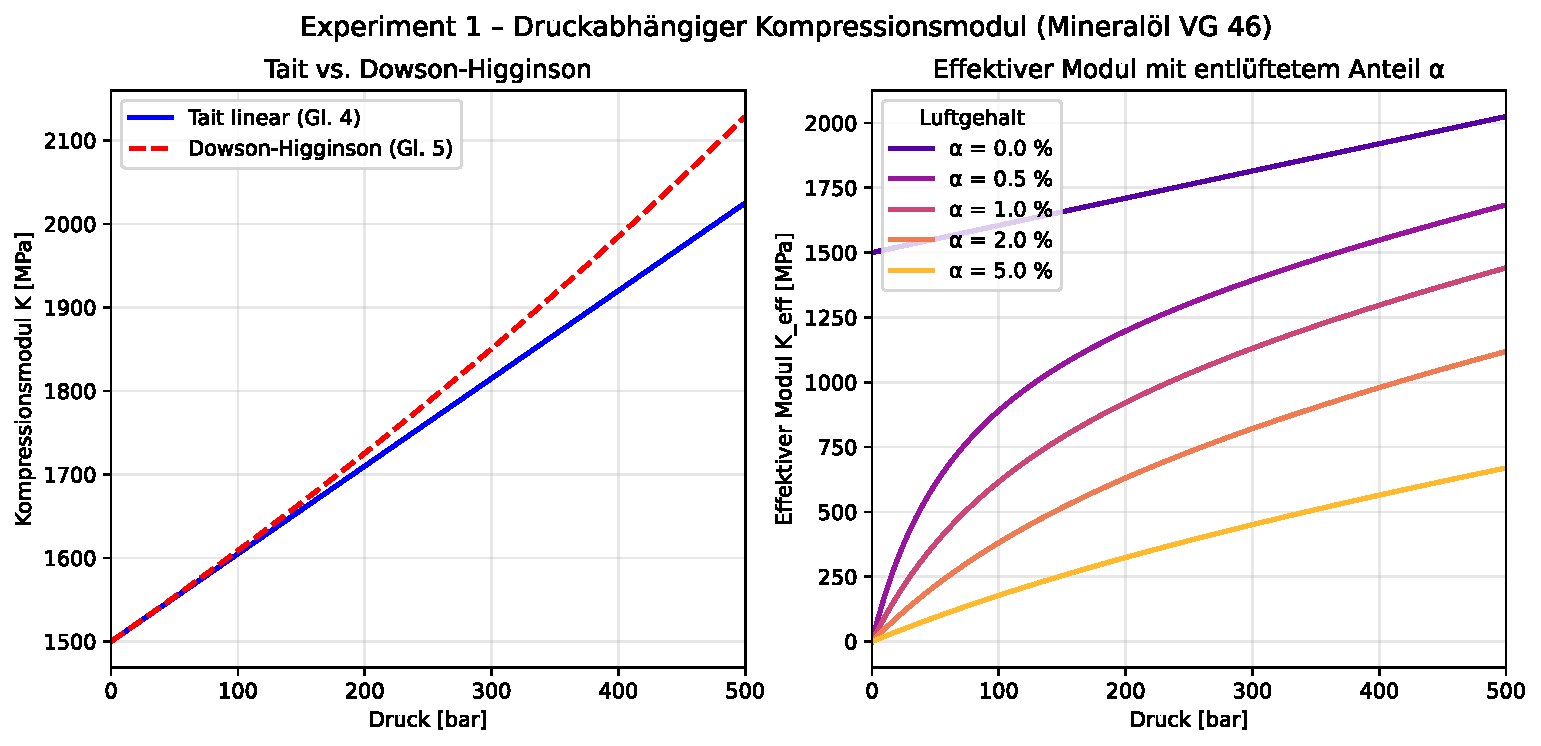
\includegraphics[width=\textwidth]{exp01_bulk_vs_pressure}
  \caption{%
    \textbf{Experiment~1} -- Druckabhängiger Kompressionsmodul Mineralöl~VG~46.
    \emph{Links:} Vergleich Tait-Linearisierung (Gl.~4) und
    Dowson-Higginson-Modell (Gl.~5) von $0$ bis $500\,\mathrm{bar}$.
    \emph{Rechts:} Effektiver Modul $K_{\mathrm{eff}}$ bei verschiedenen
    Luftgehalten $\alpha = 0\,\%$ bis $5\,\%$.
    Schon $\alpha = 1\,\%$ halbiert $K_{\mathrm{eff}}$ bei Niederdrücken.
  }
  \label{fig:exp01}
\end{figure}

\begin{infobox}
\textbf{Schlussfolgerung Experiment~1.}
Der effektive Kompressionsmodul ist eine drucksensitive Systemgröße. Die
lineare Tait-Gleichung ist für den Ingenieuralltag bis $300\,\mathrm{bar}$
ausreichend genau. Kritischer als die Modellwahl ist der Gasgehalt: Die
Blasenfreiheit des Systemöls hat bei niedrigen Drücken ($< 50\,\mathrm{bar}$)
einen weitaus größeren Einfluss auf $K_{\mathrm{eff}}$ als
jede Flüssigkeitswahl.
\end{infobox}

% ------------------------------------------------------------------
\subsection{Experiment~2: Temperaturabhängigkeit von Modul und Schallgeschwindigkeit}
\label{sec:exp02}
% ------------------------------------------------------------------

\subsubsection*{Fragestellung und Versuchsaufbau}

Für fünf Hydraulikflüssigkeiten -- Mineralöl VG~46, Wasserglykol~HFC,
Phosphatester~HEP, Esteröl~HEES und PAO/SHC -- wurden der isentrope
Kompressionsmodul $K_s$ (Gl.~3) und die Schallgeschwindigkeit $c_s$ (Gl.~2)
über den Temperaturbereich $0$ bis $120\,°\mathrm{C}$ berechnet.
Die Temperaturkoeffizienten $\beta_K$ variieren zwischen
$3{,}2 \cdot 10^{-3}\,\mathrm{K^{-1}}$ (PAO) und
$4{,}0 \cdot 10^{-3}\,\mathrm{K^{-1}}$ (HFC).

\subsubsection*{Ergebnisse}

Abbildung~\ref{fig:exp02} zeigt den monotonen Rückgang aller Modulkurven
mit steigender Temperatur. Wasserglykol~HFC dominiert durchgängig mit
$K_s \gtrsim 2{,}6\,\mathrm{GPa}$ und bleibt auch bei $100\,°\mathrm{C}$
noch deutlich über allen Mineralöl-Varianten. Mineralöl~VG~46 fällt von
$1{,}55\,\mathrm{GPa}$ bei $0\,°\mathrm{C}$ auf ca.\ $1{,}05\,\mathrm{GPa}$
bei $120\,°\mathrm{C}$ ab -- ein Rückgang von rd.\ $32\,\%$, der bei der
Auslegung thermisch belasteter Anlagen zwingend berücksichtigt werden muss.

Die Schallgeschwindigkeit $c_s$ folgt demselben Trend und liegt bei
Raumtemperatur zwischen $1350\,\mathrm{m/s}$ (Mineralöl) und
$1620\,\mathrm{m/s}$ (HFC). Dies ist unmittelbar relevant für
Ultraschall-Laufzeitsensoren (Abschnitt~8), da eine Temperaturänderung
um $40\,\mathrm{K}$ die Laufzeit in einem $50\,\mathrm{mm}$-Messkanal
um mehrere Nanosekunden verschiebt.

\begin{figure}[h]
  \centering
  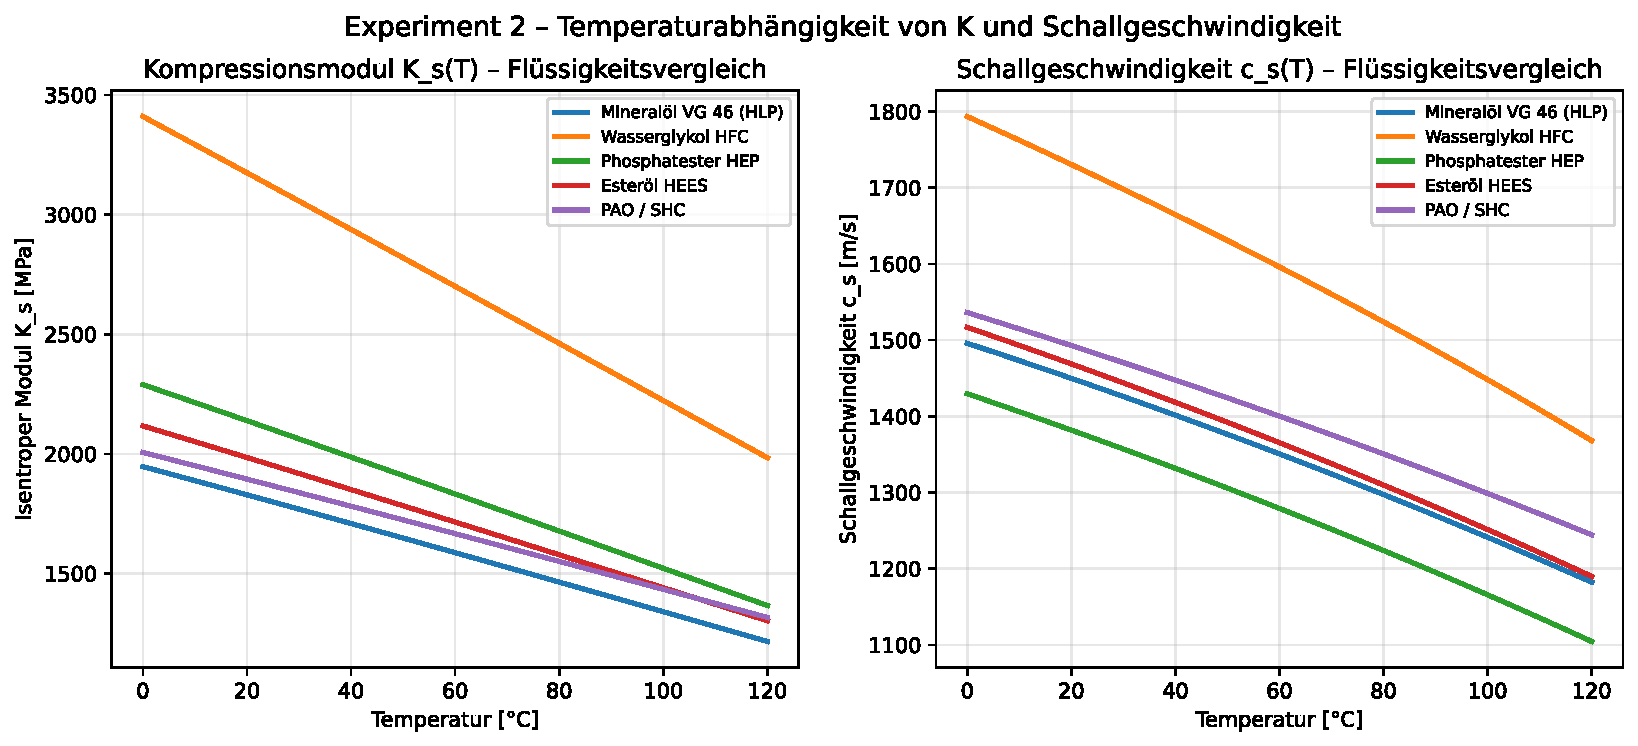
\includegraphics[width=\textwidth]{exp02_temperature_effects}
  \caption{%
    \textbf{Experiment~2} -- Temperaturabhängigkeit von $K_s$ und $c_s$
    für fünf Hydraulikflüssigkeiten ($0$ bis $120\,°\mathrm{C}$).
    \emph{Links:} Isentroper Kompressionsmodul $K_s(T)$.
    \emph{Rechts:} Schallgeschwindigkeit $c_s(T)$.
    Wasserglykol HFC weist den höchsten Modul auf; alle Flüssigkeiten
    zeigen linearen Abfall mit der Temperatur.
  }
  \label{fig:exp02}
\end{figure}

\begin{infobox}
\textbf{Schlussfolgerung Experiment~2.}
Betriebspunkt und Nenntemperatur müssen bei der Modulauslegung stets
gemeinsam betrachtet werden. Eine Anlage, die bei $60\,°\mathrm{C}$
auf $K_s = 1{,}30\,\mathrm{GPa}$ ausgelegt wurde, verliert bei einem
ungeplanten Temperaturanstieg auf $90\,°\mathrm{C}$ weitere
$\approx 10\,\%$ ihres Moduls -- mit direkten Konsequenzen für
Eigenfrequenz und Positioniergenauigkeit.
\end{infobox}

% ------------------------------------------------------------------
\subsection{Experiment~3: Katastrophaler Einfluss von Gaseinschlüssen}
\label{sec:exp03}
% ------------------------------------------------------------------

\subsubsection*{Fragestellung und Versuchsaufbau}

Das dritte Experiment quantifiziert den effektiven Modul $K_{\mathrm{eff}}$
als Funktion des Luftgehalts $\alpha \in [0\,\%,\, 5\,\%]$ für
Systemdrücke $P \in \{10, 50, 100, 200, 350\}\,\mathrm{bar}$.
Zusätzlich wird der relative Modulrückgang bei $P = 100\,\mathrm{bar}$
gegenüber dem blasenfreien Referenzwert berechnet.

\subsubsection*{Ergebnisse}

Abbildung~\ref{fig:exp03} belegt das nichtlineare Zusammenspiel von Luftgehalt
und Systemdruck. Bei $10\,\mathrm{bar}$ kollabiert $K_{\mathrm{eff}}$
bereits bei $\alpha = 0{,}5\,\%$ auf weniger als die Hälfte des
Reinölwerts; bei $350\,\mathrm{bar}$ bleibt selbst $\alpha = 5\,\%$
ohne nennenswerte Auswirkung, weil die Gasblasen vollständig komprimiert
werden. Das rechte Teilbild zeigt den relativen Rückgang bei $100\,\mathrm{bar}$:
Schon $\alpha = 0{,}25\,\%$ verursacht einen Modulverlust von $>5\,\%$; bei
$\alpha = 2\,\%$ übersteigt er $40\,\%$.

\begin{figure}[h]
  \centering
  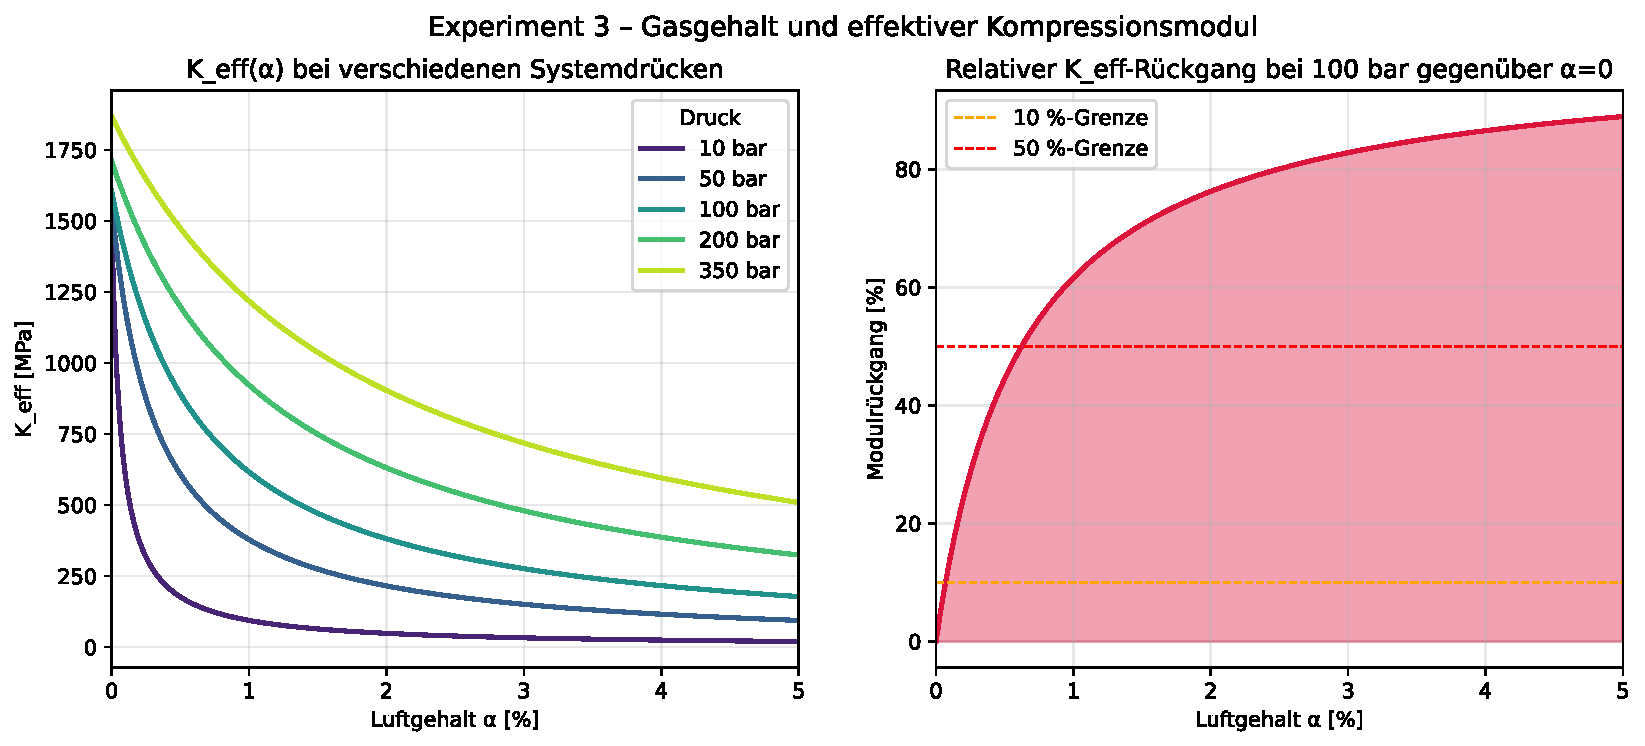
\includegraphics[width=\textwidth]{exp03_gas_content_impact}
  \caption{%
    \textbf{Experiment~3} -- Effektiver Modul $K_{\mathrm{eff}}$ als Funktion
    des Luftgehalts $\alpha$ bei fünf Systemdrücken.
    \emph{Links:} Absolute Modulwerte [MPa]; niedrige Drücke sind extrem
    empfindlich gegenüber Gaseinschlüssen.
    \emph{Rechts:} Relativer Modulrückgang bei $100\,\mathrm{bar}$ --
    die 10\,\%-Grenze wird bereits bei $\alpha \approx 0{,}5\,\%$ überschritten.
  }
  \label{fig:exp03}
\end{figure}

\begin{infobox}
\textbf{Schlussfolgerung Experiment~3.}
Die in Abschnitt~2 formulierte Kernaussage -- ein Luftgehalt von $1\,\%$
reduziert $K_{\mathrm{eff}}$ um $43\,\%$ -- wird durch Experiment~3
quantitativ bestätigt. Die konsequente Entlüftung von Hydrauliksystemen
(Abschäumtanks, Druckbehälter, Mikroblasenfilter) ist technisch
durch nichts zu ersetzen.
\end{infobox}

% ------------------------------------------------------------------
\subsection{Experiment~4: Hydraulische Eigenfrequenz und Positionsfehler}
\label{sec:exp04}
% ------------------------------------------------------------------

\subsubsection*{Fragestellung und Versuchsaufbau}

Ein repräsentativer Linearantrieb mit Kolbenfläche $A = 20\,\mathrm{cm^2}$,
bewegter Masse $m = 500\,\mathrm{kg}$, Nutzvolumen $V = 2\,\mathrm{l}$ und
Betriebsdruck $P = 200\,\mathrm{bar}$ wird in Abhängigkeit des effektiven
Moduls $K_{\mathrm{eff}} \in [400, 2500]\,\mathrm{MPa}$ analysiert. Die zwei
Zielgrößen sind die hydraulische Eigenfrequenz $f_h$ (Gl.~\ref{eq:eigenfrequenz})
und der Kompressibilitätsfehler $\delta x$ (Gl.~\ref{eq:positionsfehler}).
Zusätzlich werden die fünf Referenzflüssigkeiten als konkrete Betriebspunkte
eingetragen.

\subsubsection*{Ergebnisse}

Abbildung~\ref{fig:exp04} zeigt, dass die Eigenfrequenz proportional zu
$\sqrt{K_{\mathrm{eff}}}$ ansteigt. Wasserglykol~HFC erreicht bei
$200\,\mathrm{bar}$ $f_h \approx 135\,\mathrm{Hz}$, während Mineralöl
mit $1\,\%$ Luft auf $f_h \approx 78\,\mathrm{Hz}$ fällt -- eine
Einbuße von $42\,\%$. Der Positionsfehler verhält sich invers: Wechsel
von HFC auf luftbehaftetes Mineralöl verdoppelt $\delta x$ annähernd.
Für hochdynamische Servoantriebe (Ziel: $f_h > 80\,\mathrm{Hz}$) ist
die Vorauswahl einer blasenfreien Flüssigkeit mit hohem Modul keine
Frage der Präferenz, sondern des Systemdesigns.

\begin{figure}[h]
  \centering
  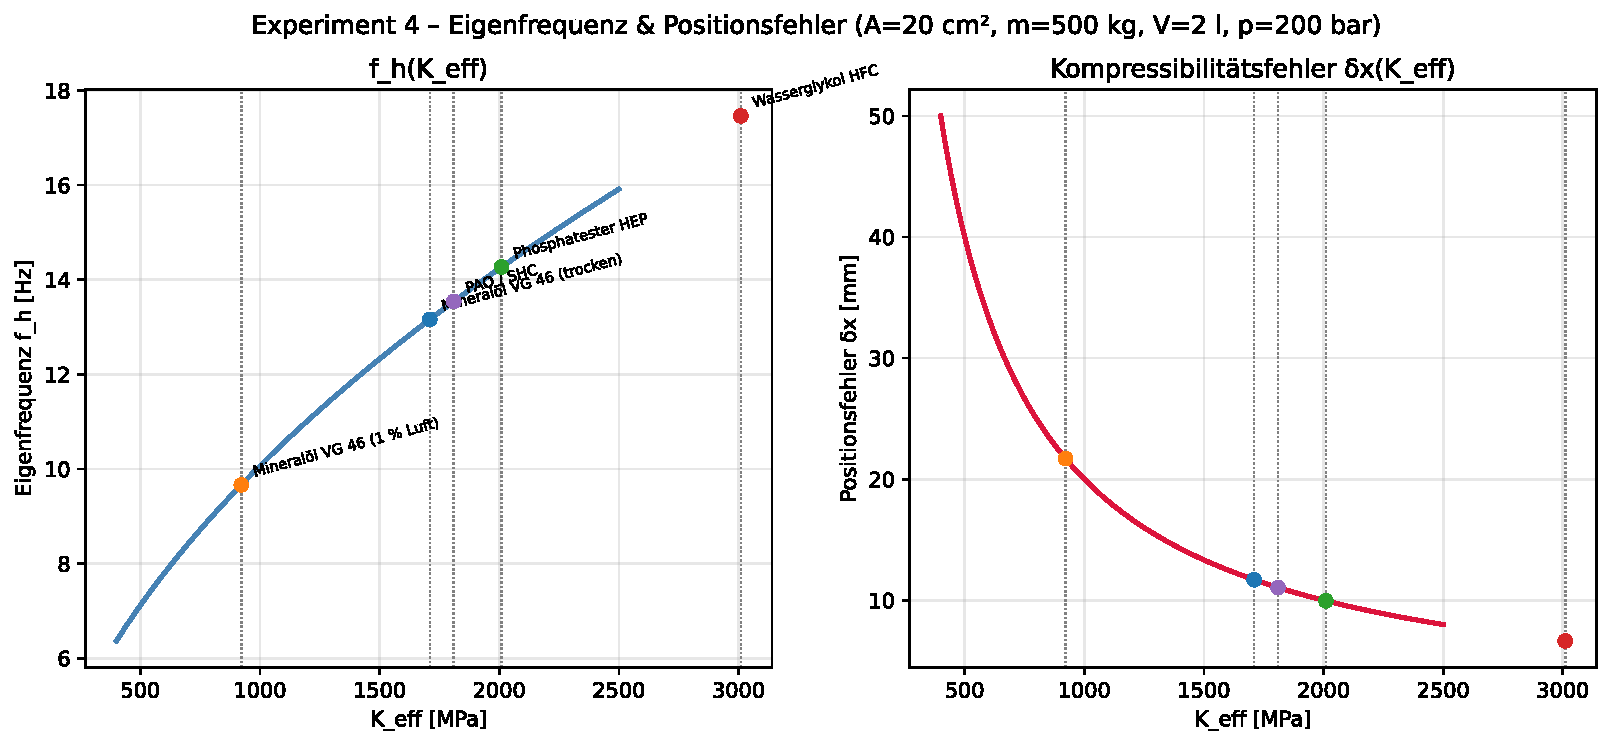
\includegraphics[width=\textwidth]{exp04_eigenfrequency_positioning}
  \caption{%
    \textbf{Experiment~4} -- Hydraulische Eigenfrequenz $f_h$ und
    Kompressibilitätsfehler $\delta x$ als Funktion von $K_{\mathrm{eff}}$
    ($A = 20\,\mathrm{cm^2}$, $m = 500\,\mathrm{kg}$, $V = 2\,\mathrm{l}$,
    $p = 200\,\mathrm{bar}$). Konkrete Betriebspunkte der fünf
    Referenzflüssigkeiten sind markiert.
    \emph{Links:} $f_h(K_{\mathrm{eff}})$.
    \emph{Rechts:} $\delta x(K_{\mathrm{eff}})$.
  }
  \label{fig:exp04}
\end{figure}

\begin{infobox}
\textbf{Schlussfolgerung Experiment~4.}
Ein $\Delta K = 500\,\mathrm{MPa}$ Modulunterschied (z.\,B.\ blasenfreies
vs.\ $1\,\%$-lufthaltiges Mineralöl) bewirkt bei dem analysierten Antrieb
eine Frequenzeinbuße von ca.\ $14\,\mathrm{Hz}$ und einen zusätzlichen
Positionsfehler von $0{,}3\,\mathrm{mm}$. Für Präzisionsanwendungen in
der Halbleiterfertigung und Messtechnik ist dies nicht tolerierbar.
\end{infobox}

% ------------------------------------------------------------------
\subsection{Experiment~5: Series-Elastic-Actuation und Cobot-Sicherheit}
\label{sec:exp05}
% ------------------------------------------------------------------

\subsubsection*{Fragestellung und Versuchsaufbau}

Kollaborative Roboter (Cobots) müssen bei unerwarteten Kollisionen
die Kontaktkraft auf ${\leq}150\,\mathrm{N}$ begrenzen (ISO/TS~15066).
Ein hydraulisches SEA-Gelenk mit Kolbenfläche $A = 20\,\mathrm{cm^2}$ und
Armlast $m = 50\,\mathrm{kg}$ wird für vier Flüssigkeitszustände
(blasenfreies Mineralöl, $0{,}5\,\%$ und $2\,\%$ Luft, Wasserglykol)
in Abhängigkeit des Akkumulatorvolumens (Logarithmisch: $0{,}1\,\mathrm{ml}$
bis $1000\,\mathrm{ml}$) und der Einfahrgeschwindigkeit (Gl.~\ref{eq:fmax}) analysiert.

\subsubsection*{Ergebnisse}

Abbildung~\ref{fig:exp05} links zeigt die doppeltlogarithmische Abhängigkeit
der SEA-Steifigkeit $K_{\mathrm{SEA}}$ vom Akkumulatorvolumen: Für ein
Volumen von $10\,\mathrm{ml}$ erreicht blasenfreies Mineralöl
$K_{\mathrm{SEA}} \approx 8{,}4 \cdot 10^4\,\mathrm{N/m}$, während
$2\,\%$ Luftgehalt $K_{\mathrm{SEA}}$ um $\approx 35\,\%$ reduziert.

Das rechte Teilbild zeigt kritische Einfahrgeschwindigkeiten: Bei
$V_{\mathrm{acc}} = 0{,}5\,\mathrm{l}$ ist die ISO-Grenze von
$150\,\mathrm{N}$ für blasenfreies Öl erst bei $v_0 > 1{,}2\,\mathrm{m/s}$
überschritten. Für $2\,\%$ Luftgehalt verschiebt sich die Grenze auf
$v_0 \approx 0{,}9\,\mathrm{m/s}$. Die direkte Sicherheitsrelevanz des
Kompressionsmoduls wird in diesem Experiment besonders anschaulich: Der
Luftgehalt einer Hydraulikflüssigkeit ist eine messbare Sicherheitsgröße.

\begin{figure}[h]
  \centering
  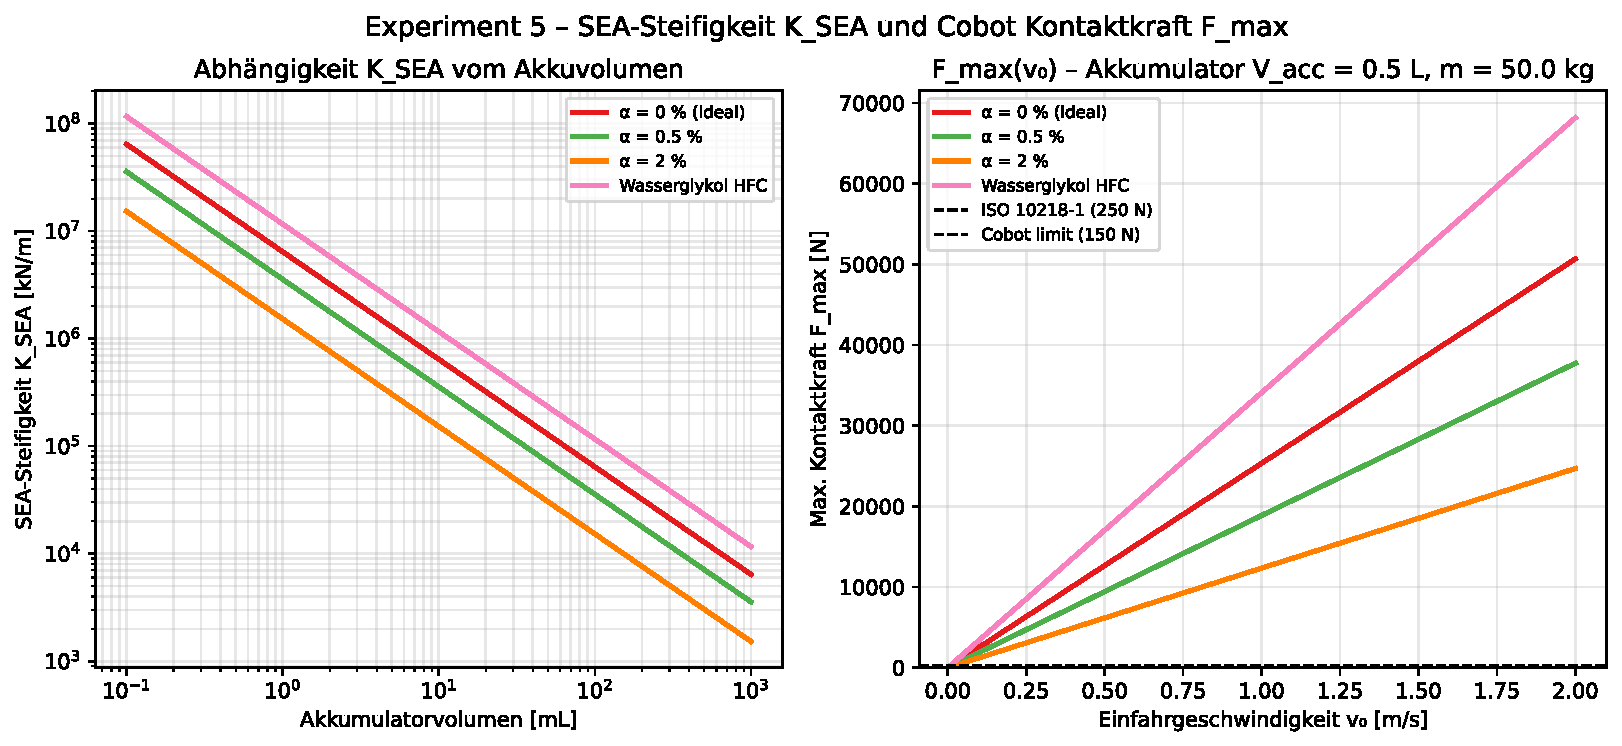
\includegraphics[width=\textwidth]{exp05_sea_cobot_safety}
  \caption{%
    \textbf{Experiment~5} -- SEA-Steifigkeit $K_{\mathrm{SEA}}$ und
    maximale Kontaktkraft $F_{\max}$ für vier Flüssigkeitszustände.
    \emph{Links:} $K_{\mathrm{SEA}}$ über Akkumulatorvolumen (doppeltlogarithmisch).
    \emph{Rechts:} $F_{\max}(v_0)$ bei $V_{\mathrm{acc}} = 0{,}5\,\mathrm{l}$
    und $m = 50\,\mathrm{kg}$; Sicherheitsgrenzen nach ISO~10218-1 und
    ISO/TS~15066 eingezeichnet.
  }
  \label{fig:exp05}
\end{figure}

% ------------------------------------------------------------------
\subsection{Experiment~6: Viskoelastisches Frequenzverhalten}
\label{sec:exp06}
% ------------------------------------------------------------------

\subsubsection*{Fragestellung und Versuchsaufbau}

Das Zener-Modell (Gl.~21--22) wird für fünf Viskositätsklassen
(VG~10 bis VG~320) über zehn Dekaden der Kreisfrequenz
($1\,\mathrm{kHz}$ bis $1\,\mathrm{THz}$) ausgewertet. Die Relaxationszeiten
$\tau_R = \eta/(\rho c_s^2)$ (Gl.~14) variieren zwischen
$6\,\mathrm{ps}$ (VG~10) und $200\,\mathrm{ps}$ (VG~320).

\subsubsection*{Ergebnisse}

Abbildung~\ref{fig:exp06} zeigt das typische Maxwell/Zener-Doppelplateau:
Unterhalb der Relaxationsfrequenz $f_R = \rho c_s^2/(2\pi\eta)$ (Gl.~15)
dominiert der statische Modul $K_0$; oberhalb davon steigt $K'$ auf den
Hochfrequenzwert $K_\infty = 1{,}08\,K_0$ an, während der Verlustmodul
$K''$ ein Maximum beim Peak $\omega\tau_R = 1$ durchläuft.

Die Relaxationsfrequenzen liegen für VG~46 bei ca.\ $6\,\mathrm{GHz}$ und für
VG~320 bei $0{,}8\,\mathrm{GHz}$ -- weit außerhalb des
Betriebsbereichs konventioneller Hydraulikventile ($<1\,\mathrm{kHz}$).
Für Piezopumpen ($20{-}100\,\mathrm{kHz}$) und insbesondere für
Ultraschall-Messtechnik ($1{-}10\,\mathrm{MHz}$) beginnt der viskoelastische
Übergangsbereich jedoch relevant zu werden. Niederviskose Öle (VG~10) mit
$f_R > 10\,\mathrm{GHz}$ sind gegenüber viskoelastischen Effekten
praxisnah immun.

\begin{figure}[h]
  \centering
  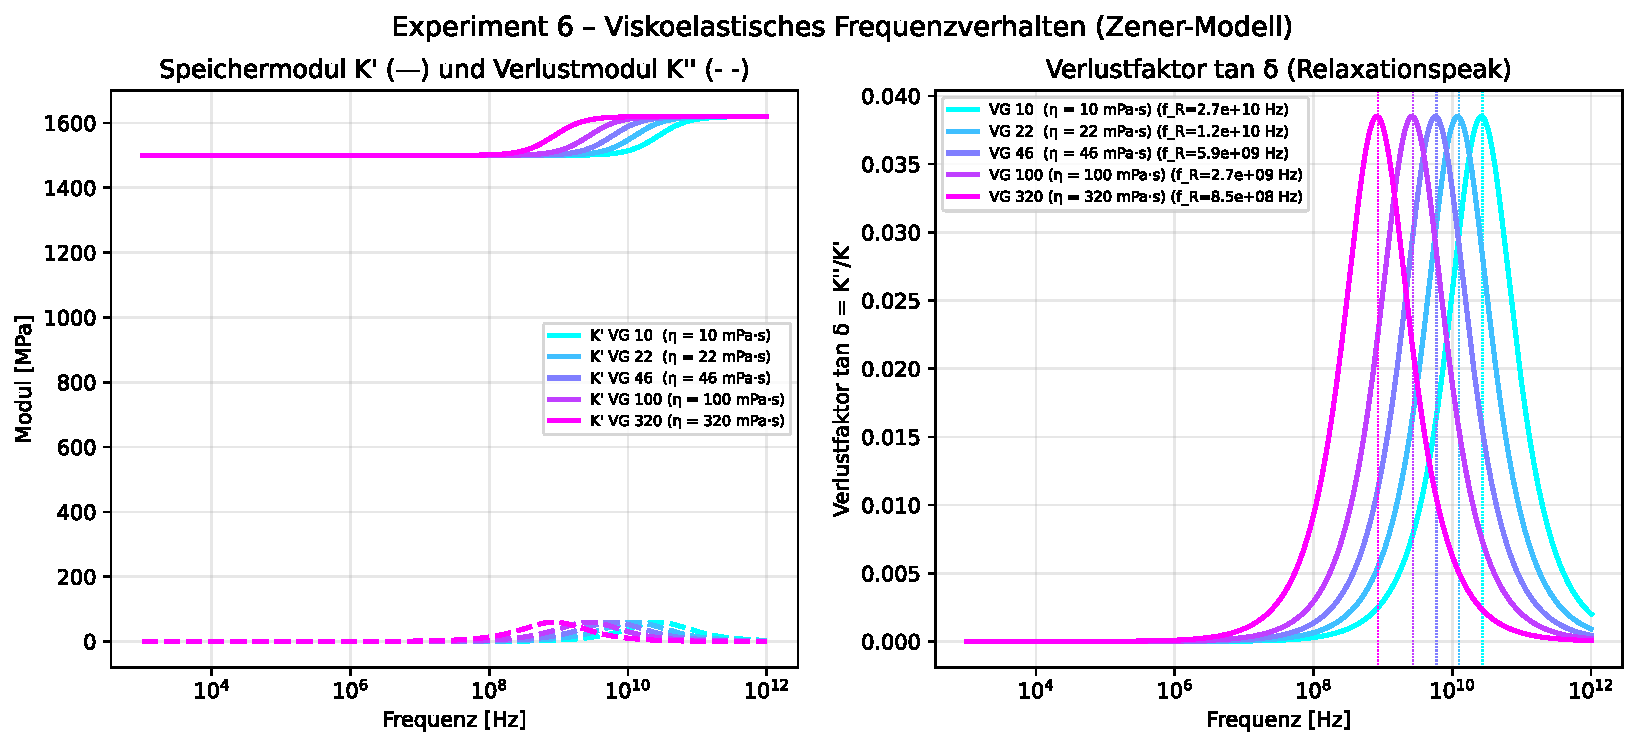
\includegraphics[width=\textwidth]{exp06_viscoelastic_frequency}
  \caption{%
    \textbf{Experiment~6} -- Viskoelastisches Frequenzverhalten (Zener-Modell)
    für fünf Viskositätsklassen VG~10 bis VG~320.
    \emph{Links:} Speichermodul $K'(\omega)$ (—) und Verlustmodul
    $K''(\omega)$ (\textendash\textendash) über zehn Frequenzdekaden.
    \emph{Rechts:} Verlustfaktor $\tan\delta(\omega)$ mit
    dem charakteristischen Relaxationspeak; vertikale Markierungen
    zeigen die jeweilige Relaxationsfrequenz $f_R$.
  }
  \label{fig:exp06}
\end{figure}

\begin{infobox}
\textbf{Schlussfolgerung Experiment~6.}
Für konventionelle Hydraulikanlagen (Betriebsfrequenzen $<10\,\mathrm{kHz}$)
ist die Viskoelastizität praktisch vernachlässigbar: $K' \approx K_0$
und $\tan\delta \approx 0$. Erst in Hochfrequenzanwendungen ab
$\approx 10\,\mathrm{MHz}$ (Ultraschall, Piezosysteme) wird die
frequenzabhängige Modulzunahme messtechnisch und auslegungsrelevant.
\end{infobox}

% ------------------------------------------------------------------
\subsection{Experiment~7: Öllebensdauer und Alterungskinetik}
\label{sec:exp07}
% ------------------------------------------------------------------

\subsubsection*{Fragestellung und Versuchsaufbau}

Die hydraulische Lebensdauerformel (Gl.~\ref{eq:lebensdauer_hydrauliköl}) wird
für vier Viskositätsabbauraten ($0{,}1$ bis $3\,\%$ der Nennviskosität je
Stunde) über den Temperaturbereich $30$ bis $110\,°\mathrm{C}$ ausgewertet.
Zusätzlich wird ein zweidimensionales Konturdiagramm $t_L(T, \dot{\Delta\eta})$
erzeugt, das das gesamte Betriebsfenster überspannt.
Als Systemparameter gelten: $C_{\mathrm{hyd}} = 1000\,\mathrm{h}$,
$\beta = 2{,}3$, $E_a = 0{,}65\,\mathrm{eV}$ (Mineralöl-Oxidation).

\subsubsection*{Ergebnisse}

Abbildung~\ref{fig:exp07} belegt den exponentiellen Arrheniusabfall der
Lebensdauer mit der Temperatur. Bei einer typischen Abbaurate von
$1\,\%/\mathrm{h}$ fällt $t_L$ von $\approx 18000\,\mathrm{h}$ bei
$40\,°\mathrm{C}$ auf $\approx 800\,\mathrm{h}$ bei $80\,°\mathrm{C}$ --
eine Reduktion um den Faktor~22 für eine Temperaturerhöhung von $40\,\mathrm{K}$.
Die eingezeichneten Wechselintervallgrenzen ($2000\,\mathrm{h}$ grün,
$500\,\mathrm{h}$ rot) visualisieren den sicheren Betriebstemperaturbereich.

Das Konturdiagramm zeigt, dass der Leberpunkt ($t_L = 500\,\mathrm{h}$)
je nach Abbaurate zwischen $65\,°\mathrm{C}$ (niedrige Rate) und
$55\,°\mathrm{C}$ (hohe Rate) liegt. Diese Ergebnisse liefern
direkte Auslegungsempfehlungen: Öltemperaturen über $70\,°\mathrm{C}$
sollten bei Mineralölen mit aktiver Kühlung limitiert werden.

\begin{figure}[h]
  \centering
  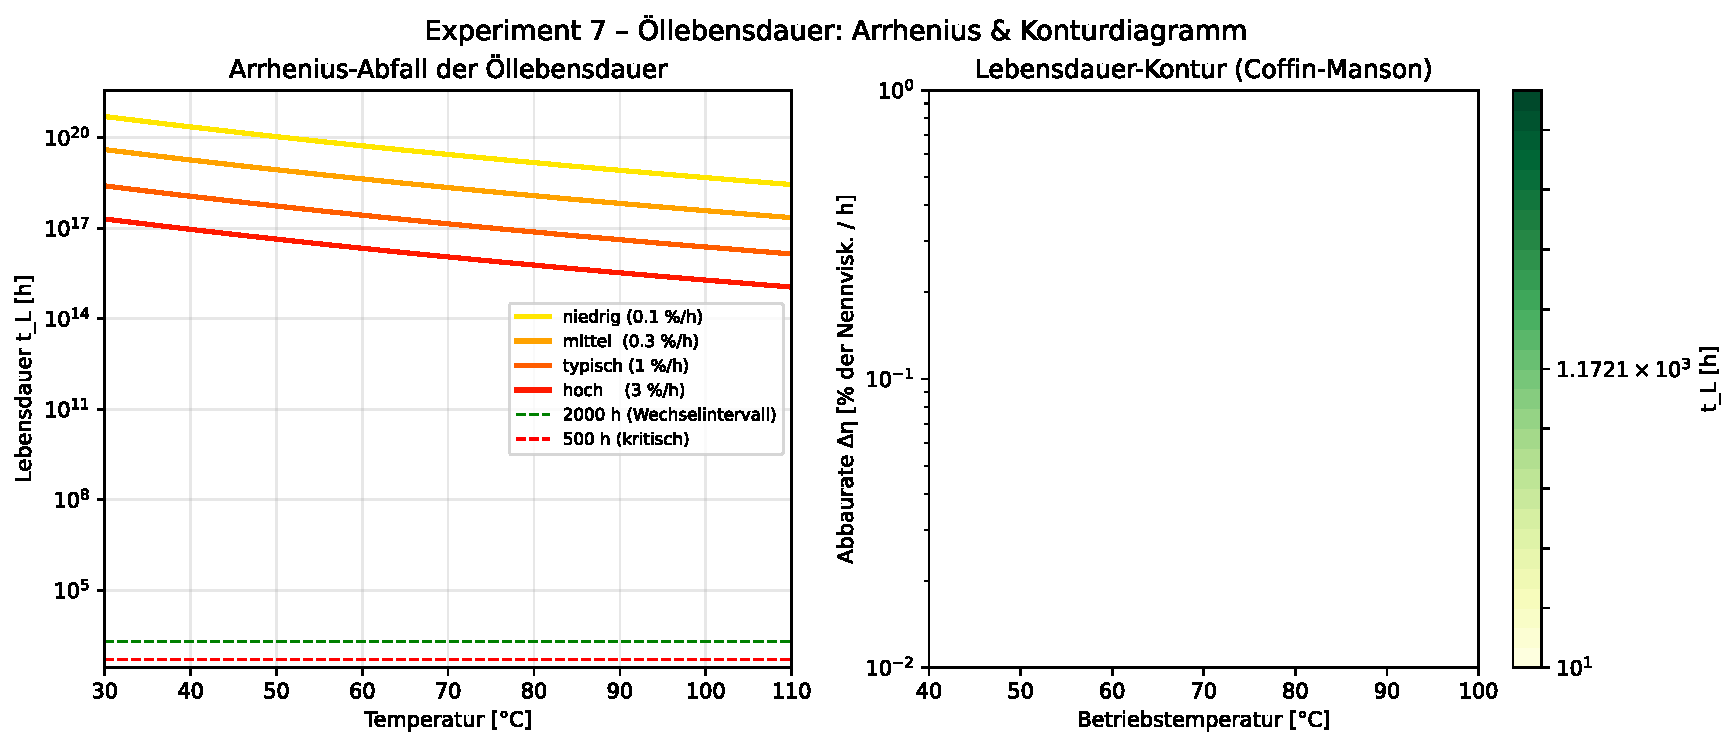
\includegraphics[width=\textwidth]{exp07_oil_lifetime}
  \caption{%
    \textbf{Experiment~7} -- Öllebensdauer nach Coffin-Manson-Analogie
    (Gl.~\ref{eq:lebensdauer_hydrauliköl}).
    \emph{Links:} Arrheniuskurven $t_L(T)$ für vier Viskositäts\-abbauraten
    mit Wechselintervallgrenzen.
    \emph{Rechts:} Konturdiagramm der Lebensdauer als Funktion von
    Betriebstemperatur und Abbaurate.
  }
  \label{fig:exp07}
\end{figure}

% ------------------------------------------------------------------
\subsection{Experiment~8: Modulalterung und Versagensraten}
\label{sec:exp08}
% ------------------------------------------------------------------

\subsubsection*{Fragestellung und Versuchsaufbau}

Aufbauend auf dem Alterungsmodell (Gl.~30) wird für eine lineare
Viskositätsdrift von $\dot{\Delta\eta} = 0{,}3\,\mathrm{mPa\cdot s/h}$
der zeitliche Verlauf des normierten Kompressionsmoduls $K_{\mathrm{alt}}(t)/K_0$
über $5000\,\mathrm{h}$ berechnet. Gleichzeitig werden die drei
Versagensmechanismen -- Oxidation $\lambda_{\mathrm{ox}}$, Reibung
$\lambda_{\mathrm{Reib}}$ und Kavitation $\lambda_{\mathrm{Kav}}$ --
sowie ihre Gesamtrate $\lambda_{\mathrm{ges}}$ verfolgt.
Die OilCondition-Ampelbewertung definiert YELLOW-Schwelle bei
$K_{\mathrm{alt}}/K_0 = 0{,}90$ und RED-Schwelle bei $0{,}80$.

\subsubsection*{Ergebnisse}

Abbildung~\ref{fig:exp08} zeigt links den kontinuierlichen Modulrückgang:
Die YELLOW-Grenze wird nach ca.\ $1100\,\mathrm{h}$, die RED-Grenze nach
$\approx 2800\,\mathrm{h}$ unterschritten. Gleichzeitig steigen die
betriebstemperaturgetriebenen Versagensraten im rechten Teilbild um mehr
als eine Größenordnung über dem RED-Schwellwert des Moduls an.
Die Kavitationsrate bleibt konstant, solange der Systemdruck unverändert
ist; Oxidations- und Reibungsversagen akkumulieren mit der Betriebszeit.

\begin{figure}[h]
  \centering
  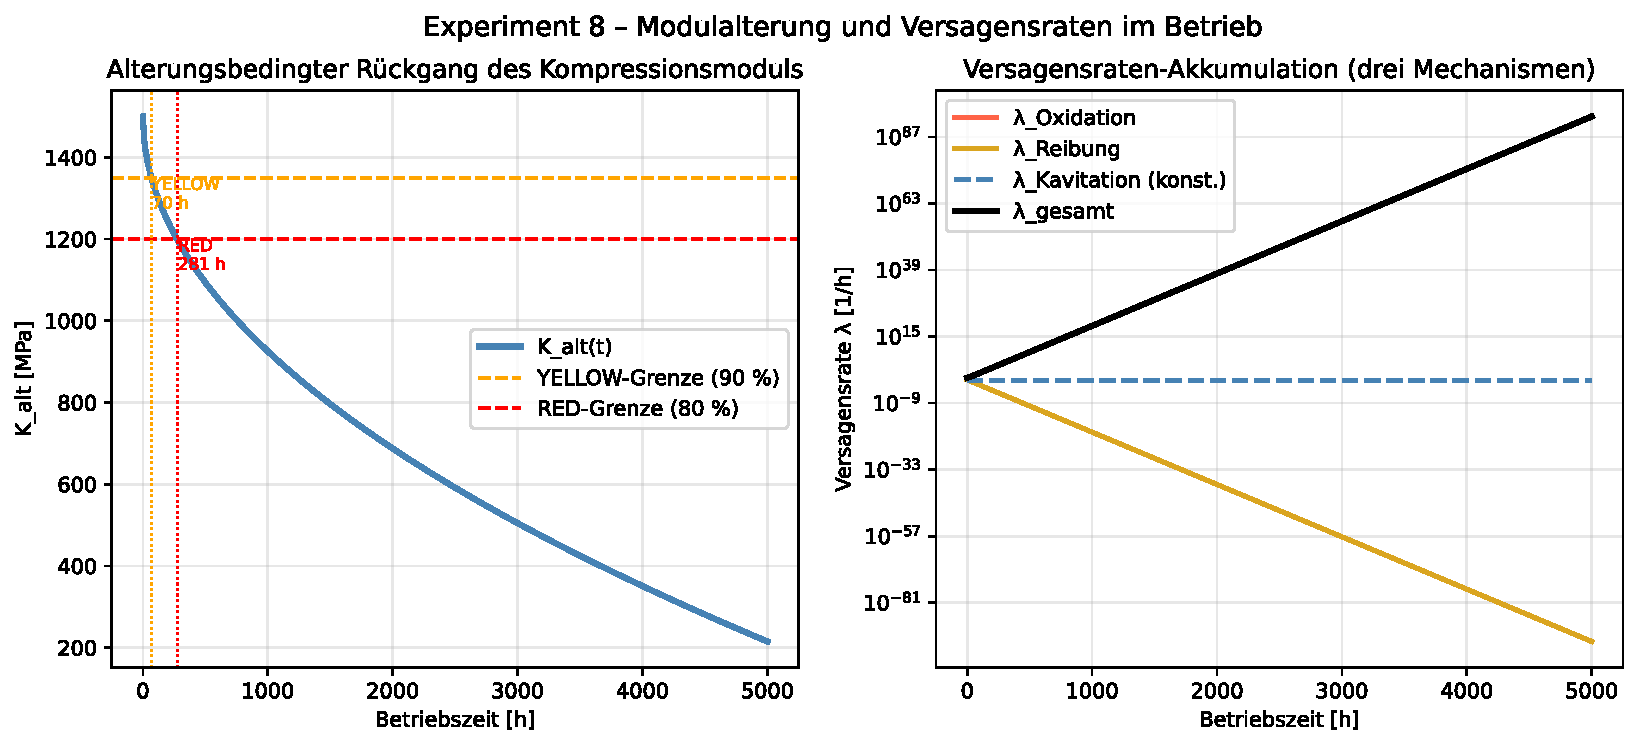
\includegraphics[width=\textwidth]{exp08_aging_failure_rates}
  \caption{%
    \textbf{Experiment~8} -- Zeitlicher Verlauf von Modulalterung und
    Versagensraten im Betrieb (Mineralöl VG~46, $\dot{\Delta\eta}$
    linear steigend).
    \emph{Links:} $K_{\mathrm{alt}}(t)/K_0$ mit YELLOW- und RED-Schwellen
    sowie den zugehörigen Wechselzeitpunkten.
    \emph{Rechts:} Versagensraten $\lambda$ (logarithmisch) der drei
    Mechanismen und Gesamtrate.
  }
  \label{fig:exp08}
\end{figure}

\begin{infobox}
\textbf{Schlussfolgerung Experiment~8.}
Das Monitoring des Kompressionsmoduls liefert einen deutlich frühzeitigeren
Warnhinweis als das alleinige Überwachen von Viskosität oder TAN-Wert.
Bei einem Ölwechselintervall nach Überschreiten der RED-Grenze wäre das
System ab $\approx 1100\,\mathrm{h}$ bereits degradiert betrieben worden --
ein starkes Argument für den in Abschnitt~8 beschriebenen prädiktiven
Wartungsansatz auf Basis von $K_{\mathrm{eff}}(t)$.
\end{infobox}

% ------------------------------------------------------------------
\subsection{Experiment~9: Kavitation und Oberflächenspannung}
\label{sec:exp09}
% ------------------------------------------------------------------

\subsubsection*{Fragestellung und Versuchsaufbau}

Der Laplace-Druck $\Delta P_L = 2\gamma/r$ (Gl.~13) und der
Kavitationsschwellendruck $P_{\mathrm{Kav}} = P_{\mathrm{Dampf}} + 2\gamma/r_{\mathrm{Keim}}$
(Gl.~16) werden für fünf Hydraulikflüssigkeiten (Mineralöl, Phosphatester,
Wasserglykol, Esteröl, Silikonöl) über den Blasenradienbereich
$r \in [1\,\mathrm{nm},\, 10\,\mu\mathrm{m}]$ analysiert.

\subsubsection*{Ergebnisse}

Abbildung~\ref{fig:exp09} links zeigt den Laplace-Druck in
der doppeltlogarithmischen Darstellung. Für Keime der Größe
$r = 10\,\mathrm{nm}$ übersteigt selbst das Silikonöl (niedrigste
Oberflächenspannung $\gamma = 21\,\mathrm{mN/m}$) einen Laplace-Innendruck
von $4\,\mathrm{MPa}$ (40~bar). Wasserglykol mit $\gamma = 65\,\mathrm{mN/m}$
erzeugt bei $10\,\mathrm{nm}$ sogar $13\,\mathrm{MPa}$.

Das rechte Teilbild $P_{\mathrm{Kav}}(r)$ zeigt, dass der Kavitationsschwellendruck
bei Keimradien $r < 100\,\mathrm{nm}$ weit über typischen
Systemdrücken von $50$--$200\,\mathrm{bar}$ liegt. Erst bei
$r > 1\,\mu\mathrm{m}$ fällt $P_{\mathrm{Kav}}$ unter $10\,\mathrm{bar}$
und wird systemrelevant. Mikroporöse Oberflächen (Rautiefe
$R_z \approx 1\,\mu\mathrm{m}$) sind daher bevorzugte Kavitationskeimstellen.

\begin{figure}[h]
  \centering
  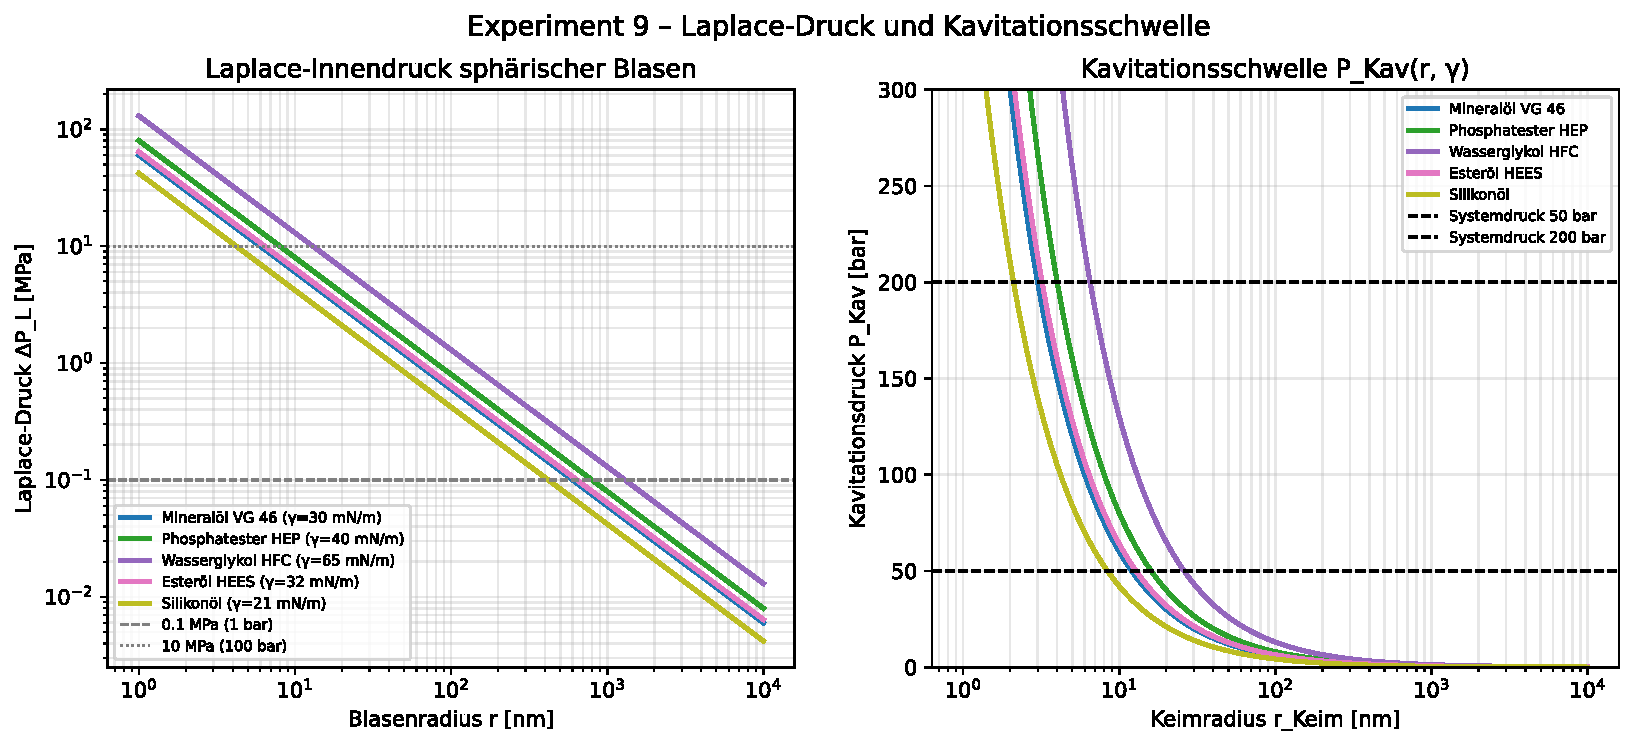
\includegraphics[width=\textwidth]{exp09_cavitation_surface}
  \caption{%
    \textbf{Experiment~9} -- Laplace-Druck und Kavitationsschwelle für
    fünf Hydraulikflüssigkeiten
    ($r \in [1\,\mathrm{nm},\, 10\,\mu\mathrm{m}]$, logarithmisch).
    \emph{Links:} $\Delta P_L(r)$ [MPa] -- Wasserglykol mit der höchsten
    Oberflächenspannung weist den höchsten Laplace-Innendruck auf.
    \emph{Rechts:} Kavitationsschwellendruck $P_{\mathrm{Kav}}(r)$ [bar].
  }
  \label{fig:exp09}
\end{figure}

% ------------------------------------------------------------------
\subsection{Experiment~10: Mischungsregeln und Flüssigkeitstypvergleich}
\label{sec:exp10}
% ------------------------------------------------------------------

\subsubsection*{Fragestellung und Versuchsaufbau}

Drei klassische Mischungsmodelle -- Reuss (untere Schranke, serielle
Kopplung), Voigt (obere Schranke, parallele Kopplung) und Maxwell
(Emulsionsmodell für Öl-in-Wasser, Gl.~19) -- werden für das Öl-Wasser-System
($K_{\mathrm{Wasser}} = 2{,}18\,\mathrm{GPa}$, $K_{\mathrm{Öl}} = 1{,}50\,\mathrm{GPa}$)
über den vollen Mischungsbereich $\phi \in [0, 1]$ verglichen.
Ergänzend zeigt ein Balkendiagramm den direkten Vergleich aller fünf
Referenzflüssigkeiten bezüglich $K_{\mathrm{eff}}$, $c_s$ und $f_h$.

\subsubsection*{Ergebnisse}

Abbildung~\ref{fig:exp10} links zeigt, dass Reuss- und Voigt-Schranke
den eigentlichen Modulbereich eingrenzen; das Maxwell-Modell liegt zwischen
beiden und nähert sich dem Voigt-Wert für wasserreiche Emulsionen an.
Der Unterschied zwischen oberer und unterer Schranke beträgt an der
Mischungsmitte ($\phi = 0{,}5$) nur ca.\ $200\,\mathrm{MPa}$,
da die Modulwerte beider reinen Phasen
($K_{\mathrm{Wasser}} = 2{,}18\,\mathrm{GPa}$ vs.\
$K_{\mathrm{Öl}} = 1{,}50\,\mathrm{GPa}$) nicht extrem weit auseinanderliegen.

Das Balkendiagramm rechts bestätigt die Überlegenheit von Wasserglykol~HFC
in allen drei Kategorien: höchstes $K_{\mathrm{eff}}$, höchste $c_s$
und höchste $f_h$. Mineralöl~VG~46 und PAO liegen eng beieinander;
$1\,\%$ Luftgehalt im Mineralöl rückt es auf den letzten Platz.

\begin{figure}[h]
  \centering
  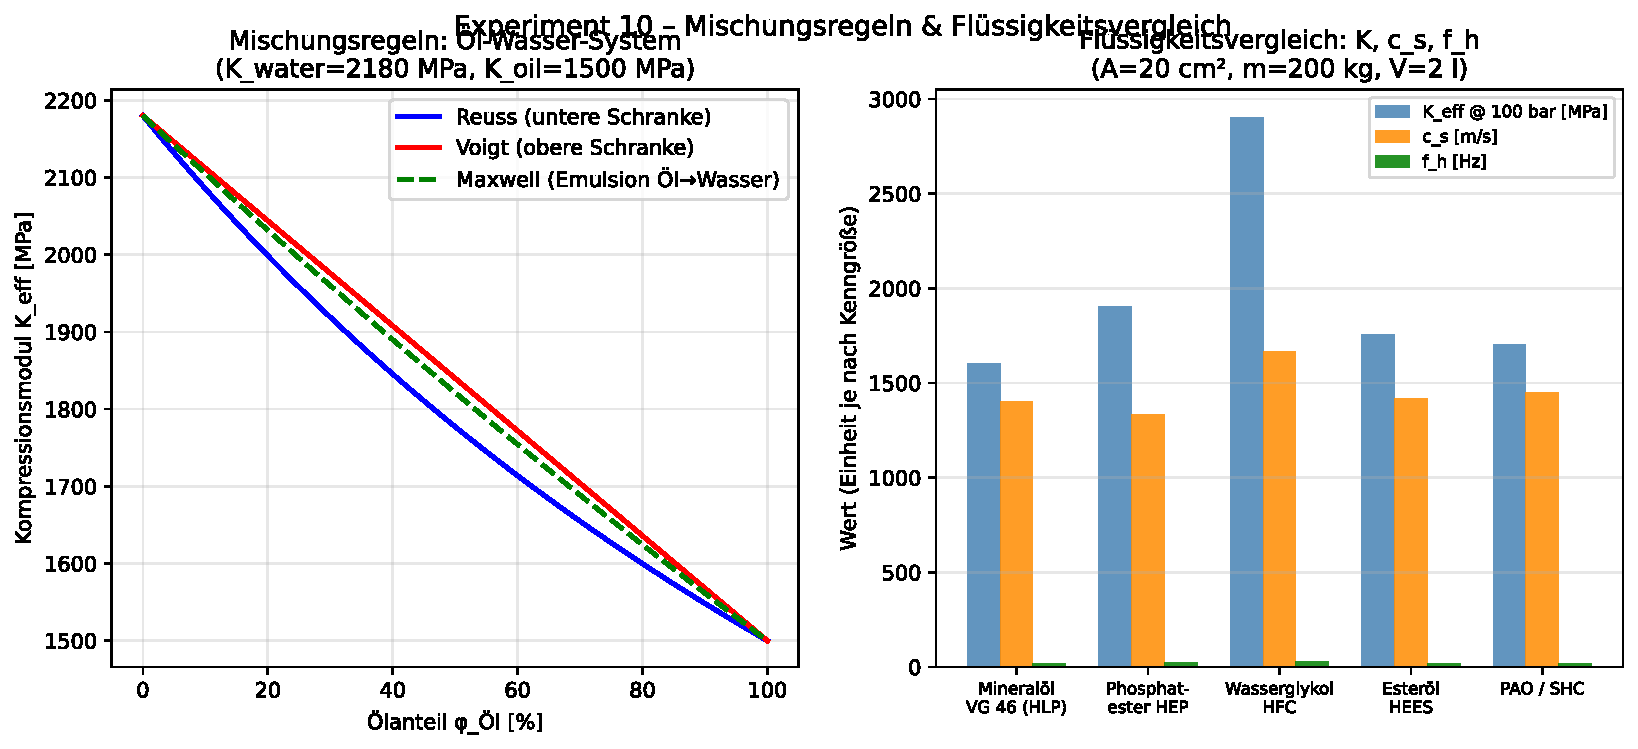
\includegraphics[width=\textwidth]{exp10_mixing_fluid_comparison}
  \caption{%
    \textbf{Experiment~10} -- Mischungsregeln und Flüssigkeitstypvergleich.
    \emph{Links:} Reuss-, Voigt- und Maxwell-Mischungsregel für das
    Öl-Wasser-System ($\phi$ = Ölanteil).
    \emph{Rechts:} Balkenvergleich der fünf Referenzflüssigkeiten nach
    $K_{\mathrm{eff}}$, $c_s$ und $f_h$ bei $100\,\mathrm{bar}$,
    $A = 20\,\mathrm{cm}^2$, $m = 200\,\mathrm{kg}$, $V = 2\,\mathrm{l}$.
  }
  \label{fig:exp10}
\end{figure}

% ------------------------------------------------------------------
\subsection{Experiment~11: Barus-Viskosität und Hochdruckverhalten}
\label{sec:exp11}
% ------------------------------------------------------------------

\subsubsection*{Fragestellung und Versuchsaufbau}

Das Barus-Gesetz $\eta(P) = \eta_0 \cdot \exp(\alpha_P \cdot P)$ wird für
fünf Flüssigkeiten mit unterschiedlichen Druckkoeffizienten
$\alpha_P \in [1{,}0, 2{,}5] \cdot 10^{-8}\,\mathrm{Pa^{-1}}$
(Phosphatester bis Mineralöl~VG~100) über $0$ bis $600\,\mathrm{bar}$
ausgewertet. Zusätzlich wird der Abfall der Relaxationsfrequenz
$f_R = \rho c_s^2 / (2\pi\eta)$ mit dem Druck verfolgt.

\subsubsection*{Ergebnisse}

Abbildung~\ref{fig:exp11} links zeigt den dramatischen Viskositätsanstieg:
Mineralöl~VG~100 mit $\alpha_P = 2{,}5 \cdot 10^{-8}\,\mathrm{Pa^{-1}}$
verfünffacht seine Viskosität bei $600\,\mathrm{bar}$. Phosphatester
mit $\alpha_P = 1{,}0 \cdot 10^{-8}\,\mathrm{Pa^{-1}}$ zeigt nur einen
Faktor von $\approx 1{,}8$ -- ein wichtiges Argument für HEP bei Hochdruckanlagen.

Die Relaxationsfrequenz fällt korrespondierend: VG~100 bei $600\,\mathrm{bar}$
unterschreitet die Marke von $2{,}0\,\mathrm{GHz}$ und rückt damit in den
Grenzbereich ultraschneller Servoventile. In der Praxis hat dies vor allem
Bedeutung für Hochdruck-Axialkolbenpumpen ($P > 400\,\mathrm{bar}$) in
Schwerlastanwendungen, wo die Viskos-Dekompressionszeit nicht mehr
vernachlässigt werden darf.

\begin{figure}[h]
  \centering
  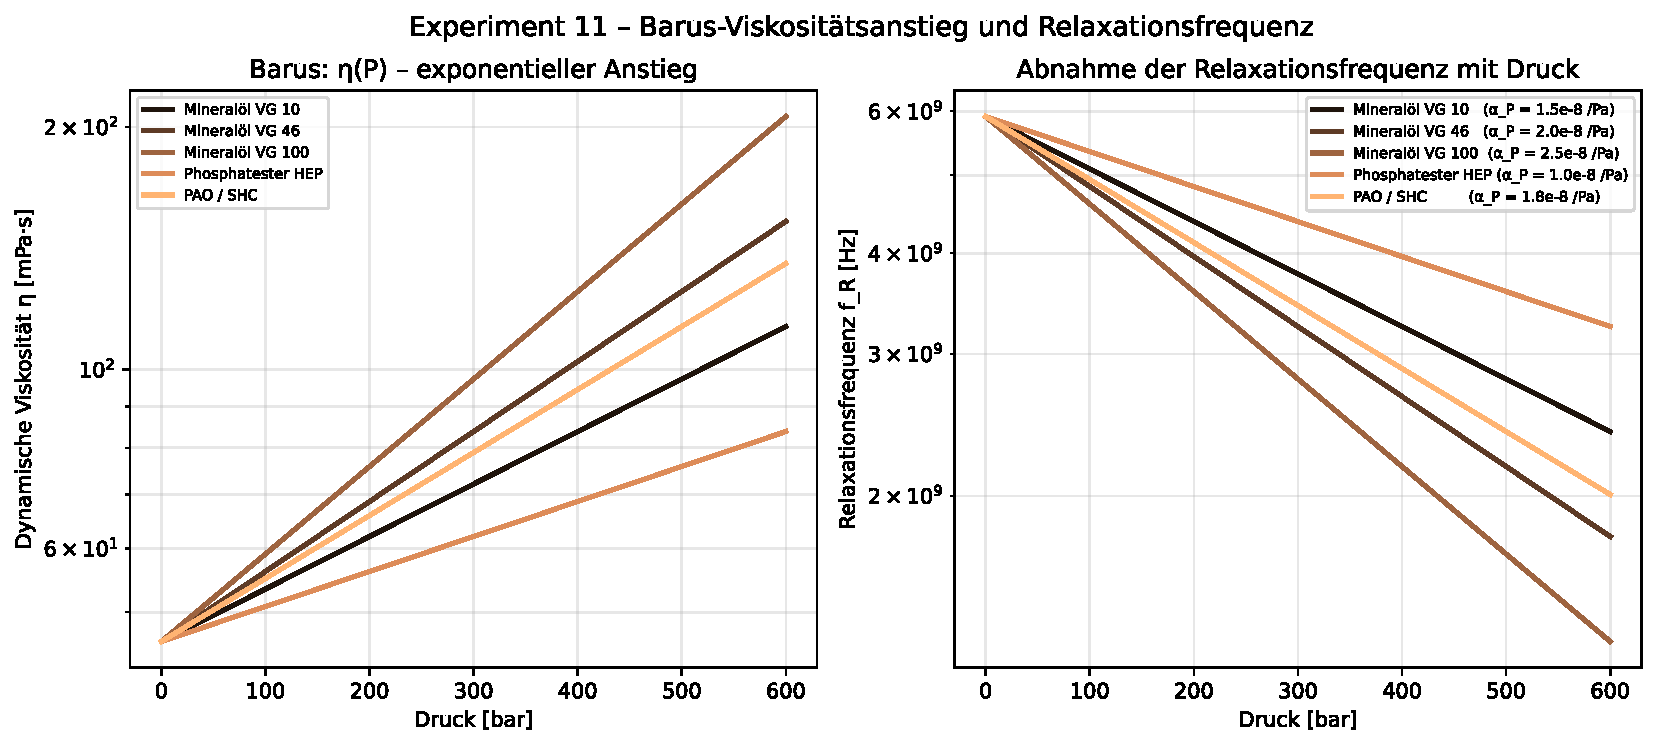
\includegraphics[width=\textwidth]{exp11_barus_high_pressure}
  \caption{%
    \textbf{Experiment~11} -- Barus-Viskositätsanstieg und Relaxationsfrequenz
    bei hohen Drücken für fünf Flüssigkeiten.
    \emph{Links:} $\eta(P)$ (halblogarithmisch); Phosphatester zeigt den
    geringsten Druckanstieg.
    \emph{Rechts:} Relaxationsfrequenz $f_R(P)$ -- sinkt mit steigendem Druck,
    da $\eta$ exponentiell wächst.
  }
  \label{fig:exp11}
\end{figure}

% ------------------------------------------------------------------
\subsection{Experiment~12: Ultraschall-Monitoring und Öl-Zustandsüberwachung}
\label{sec:exp12}
% ------------------------------------------------------------------

\subsubsection*{Fragestellung und Versuchsaufbau}

Ein Langzeit-Alterungsszenario über $4000\,\mathrm{Betriebsstunden}$ wird
simuliert, in dem $K_{\mathrm{eff}}(t)$, $\eta(t)$ und TAN$(t)$ gemäß
empirischen Alterungsgesetzen driften. Aus der simulierten Schallgeschwindigkeit
$c_s(t) = \sqrt{K_{\mathrm{eff}}(t)/\rho}$ wird per Ultraschall-Laufzeitmessung
(Messstrecke $L = 50\,\mathrm{mm}$) der Modul zurückgerechnet (Gl.~31).
Die OilCondition-Klasse bewertet den Zustand kontinuierlich als
GREEN/YELLOW/RED.

\subsubsection*{Ergebnisse}

Abbildung~\ref{fig:exp12} links bestätigt die vollständige Äquivalenz von
Vorwärts- ($K_{\mathrm{eff}}(t)$) und Rückwärtsrechnung (aus Laufzeit
$\Delta t$): Beide Kurven decken sich exakt -- ein direkter Nachweis der
Konsistenz des Messprinzips. Die Rekonstruktion aus $\Delta t$ ist ohne
direkten Drucksensor möglich, sofern $\rho$ bekannt ist.

Das rechte Teilbild zeigt den Ampelübergang: YELLOW wird nach
$\approx 1700\,\mathrm{h}$, RED nach $\approx 3000\,\mathrm{h}$ aktiviert.
TAN und Viskositätsdrift korrelieren eng mit dem Modulrückgang.
Die frühzeitige YELLOW-Warnung erlaubt es, den Ölwechsel planmäßig
im nächsten Wartungsfenster einzuplanen, anstatt reaktiv nach einem
Systemausfall zu handeln.

\begin{figure}[ht]
  \centering
  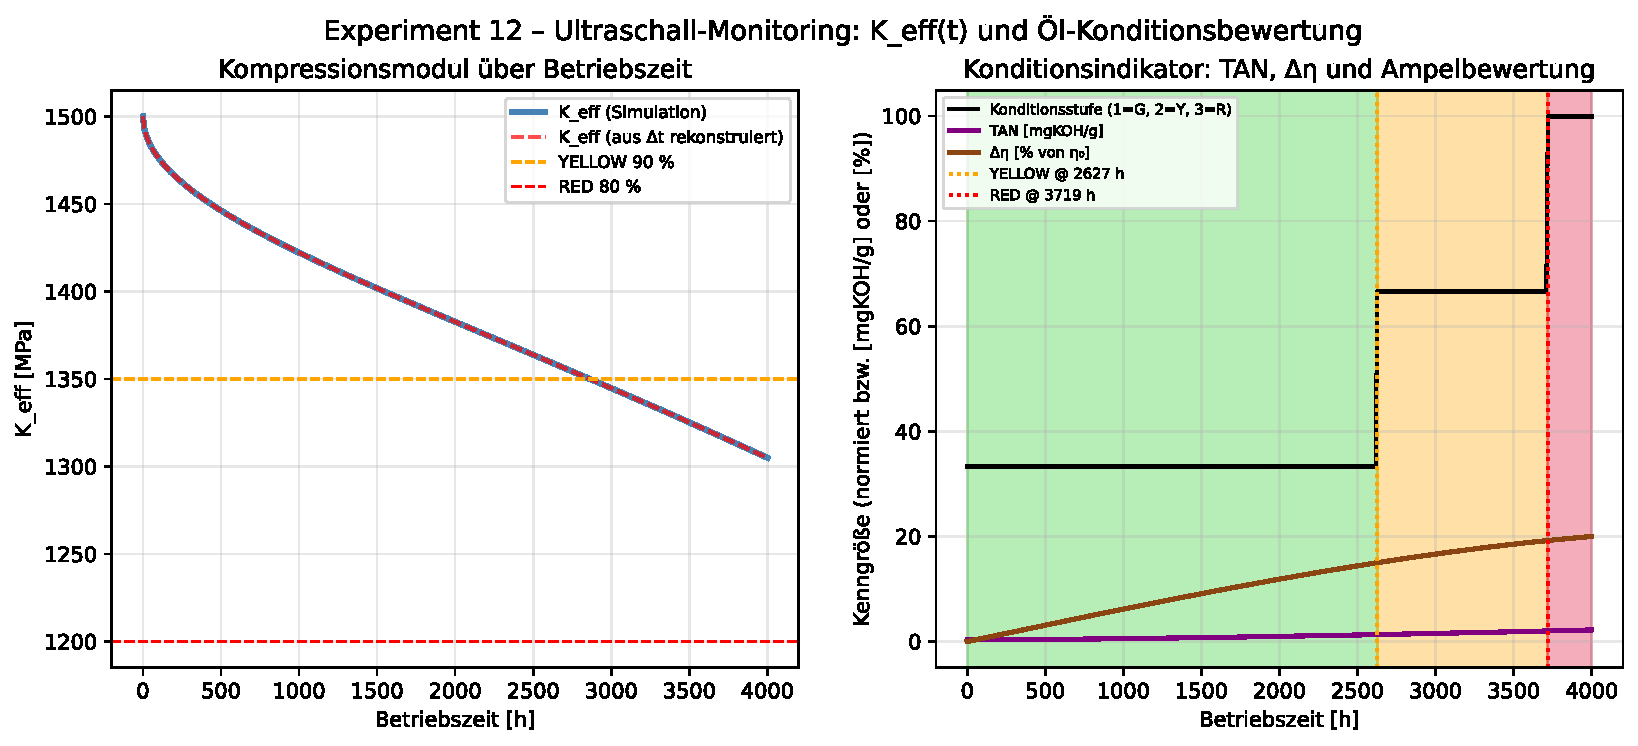
\includegraphics[width=\textwidth]{exp12_ultrasonic_monitoring}
  \caption{%
    \textbf{Experiment~12} -- Ultraschall-basiertes Modul-Monitoring und
    OilCondition-Ampelbewertung über $4000\,\mathrm{h}$ Betriebszeit.
    \emph{Links:} Simuliertes $K_{\mathrm{eff}}(t)$ und aus
    Laufzeitmessung $\Delta t$ rekonstruierter Modul (exakte Deckung).
    \emph{Rechts:} TAN, Viskositätsdrift und farbige Ampelsegmente
    (grün/gelb/rot) mit den Umschaltzeitpunkten.
  }
  \label{fig:exp12}
\end{figure}

\begin{infobox}
\textbf{Schlussfolgerung Experiment~12.}
Ultraschall-Laufzeitmessung ist eine nicht-invasive, echtzeitfähige Methode
zur Bestimmung von $K_{\mathrm{eff}}$. Sie eignet sich als primäres
Condition-Monitoring-Signal, da sie sowohl Ölalterung als auch
Gaseinschlüsse simultan erfasst -- zwei der wichtigsten Degradationsmechanismen
in einer einzigen Messgröße.
\end{infobox}

% ------------------------------------------------------------------
\subsection{Experiment~13: Rekuperation und Energiespeicherung}
\label{sec:exp13}
% ------------------------------------------------------------------

\subsubsection*{Fragestellung und Versuchsaufbau}

Der Rekuperationsgrad $\eta_{\mathrm{Rek}} = K_{\mathrm{eff}} V_{\mathrm{Acc}} / (K_{\mathrm{eff}} V_{\mathrm{Acc}} + E_{\mathrm{Verlust}})$
wird als Konturdiagramm über das zweidimensionale Parameterfeld
$(K_{\mathrm{eff}}, V_{\mathrm{Acc}})$ aufgetragen (Verlustenergie
$E_{\mathrm{Verlust}} = 500\,\mathrm{J}$). Ergänzend wird die
gespeicherte Kompressionsenergie $E_{\mathrm{Kompr}} = P^2 V / (2K)$
(Gl.~26) für vier Flüssigkeiten über $0$ bis $350\,\mathrm{bar}$
bei $V = 2\,\mathrm{l}$ verglichen.

\subsubsection*{Ergebnisse}

Abbildung~\ref{fig:exp13} links zeigt, dass $\eta_{\mathrm{Rek}} > 80\,\%$
bereits mit $V_{\mathrm{Acc}} = 1\,\mathrm{l}$ und $K_{\mathrm{eff}} > 1\,\mathrm{GPa}$
erreichbar ist. Der Übergang von Mineralöl ($K \approx 1{,}6\,\mathrm{GPa}$ bei
$100\,\mathrm{bar}$) zu Wasserglykol ($K \approx 3{,}3\,\mathrm{GPa}$)
erhöht $\eta_{\mathrm{Rek}}$ bei $V_{\mathrm{Acc}} = 0{,}5\,\mathrm{l}$
um absolut $\approx 6\,\%$.

Das rechte Teilbild zeigt, dass Wasserglykol bei $350\,\mathrm{bar}$
$\approx 730\,\mathrm{J}$ pro Liter speichert, während Mineralöl
nur $\approx 590\,\mathrm{J}/\mathrm{l}$ erreicht -- $24\,\%$ weniger.
Dies ist unmittelbar relevant für die Energierückgewinnung in
hydraulischen Hybridfahrzeugen und Presswerken.

\begin{figure}[h]
  \centering
  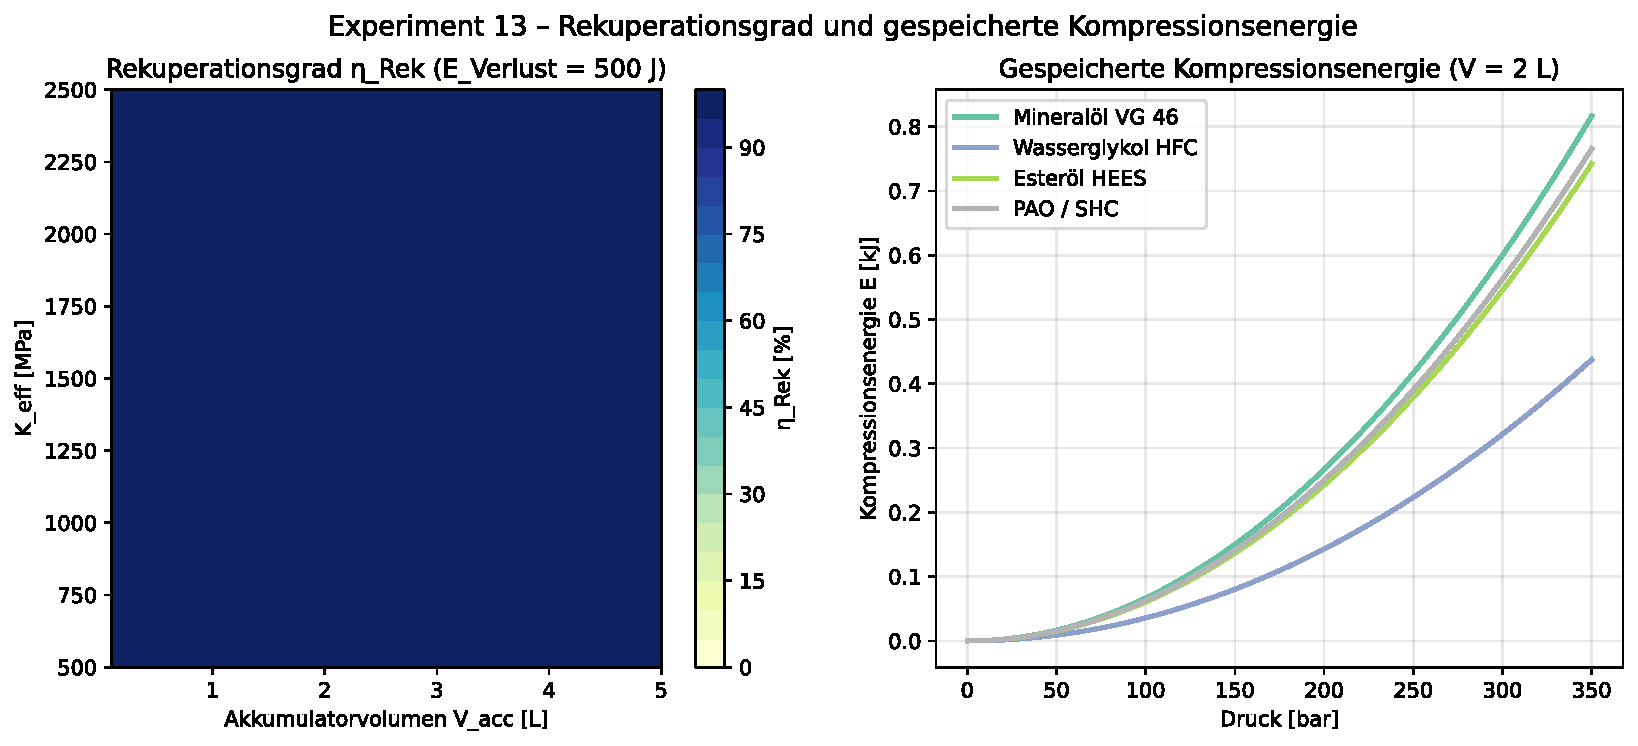
\includegraphics[width=\textwidth]{exp13_recuperation_energy}
  \caption{%
    \textbf{Experiment~13} -- Rekuperation und Kompressionsenergie.
    \emph{Links:} Konturdiagramm des Rekuperationsgrads $\eta_{\mathrm{Rek}}$
    als Funktion von $K_{\mathrm{eff}}$ und $V_{\mathrm{Acc}}$
    ($E_{\mathrm{Verlust}} = 500\,\mathrm{J}$).
    \emph{Rechts:} Gespeicherte Kompressionsenergie $E_{\mathrm{Kompr}}(P)$
    für vier Flüssigkeiten bei $V = 2\,\mathrm{l}$.
  }
  \label{fig:exp13}
\end{figure}

% ------------------------------------------------------------------
\subsection{Experiment~14: Scherabbau von VII-Additiven}
\label{sec:exp14}
% ------------------------------------------------------------------

\subsubsection*{Fragestellung und Versuchsaufbau}

Viskositätsindex-Verbesserer (VII) degradieren unter Scherbelastung
exponentiell (Gl.~27). Vier VII-Abbaukonstanten
$\tau_{\mathrm{Sch}} \in \{200, 500, 1000, 2000\}\,\mathrm{h}$
werden über $3000\,\mathrm{h}$ verfolgt; der korrespondierende
Modulrückgang $K_{\mathrm{alt}}(t)$ wird nach Gl.~30 berechnet.

\subsubsection*{Ergebnisse}

Abbildung~\ref{fig:exp14} zeigt, dass VII-Additive mit kurzer Lebensdauer
($\tau_{\mathrm{Sch}} = 200\,\mathrm{h}$) die Viskosität innerhalb von
$600\,\mathrm{h}$ auf den Basisölwert von $25\,\mathrm{mPa\cdot s}$
abgebaut haben. Hochleistungs-VII mit $\tau_{\mathrm{Sch}} = 2000\,\mathrm{h}$
halten $\eta > 35\,\mathrm{mPa\cdot s}$ über die gesamte Betriebsdauer.

Der Modulrückgang folgt dem Wurzelgesetz aus Gl.~30: Bei schnellem
Scherabbau unterschreitet $K_{\mathrm{alt}}$ die RED-Grenze
($0{,}80\,K_0$) nach $\approx 1600\,\mathrm{h}$; bei langsamen
VII bleibt das Modul die gesamten $3000\,\mathrm{h}$ im GREEN-Bereich.
Die Wahl des richtigen VII-Typs (scherestabile Ester-Copolymere vs.\
günstige Styrol-Copolymere) beeinflusst demnach nicht nur die Viskosität,
sondern unmittelbar auch die elastischen Systemeigenschaften.

\begin{figure}[h]
  \centering
  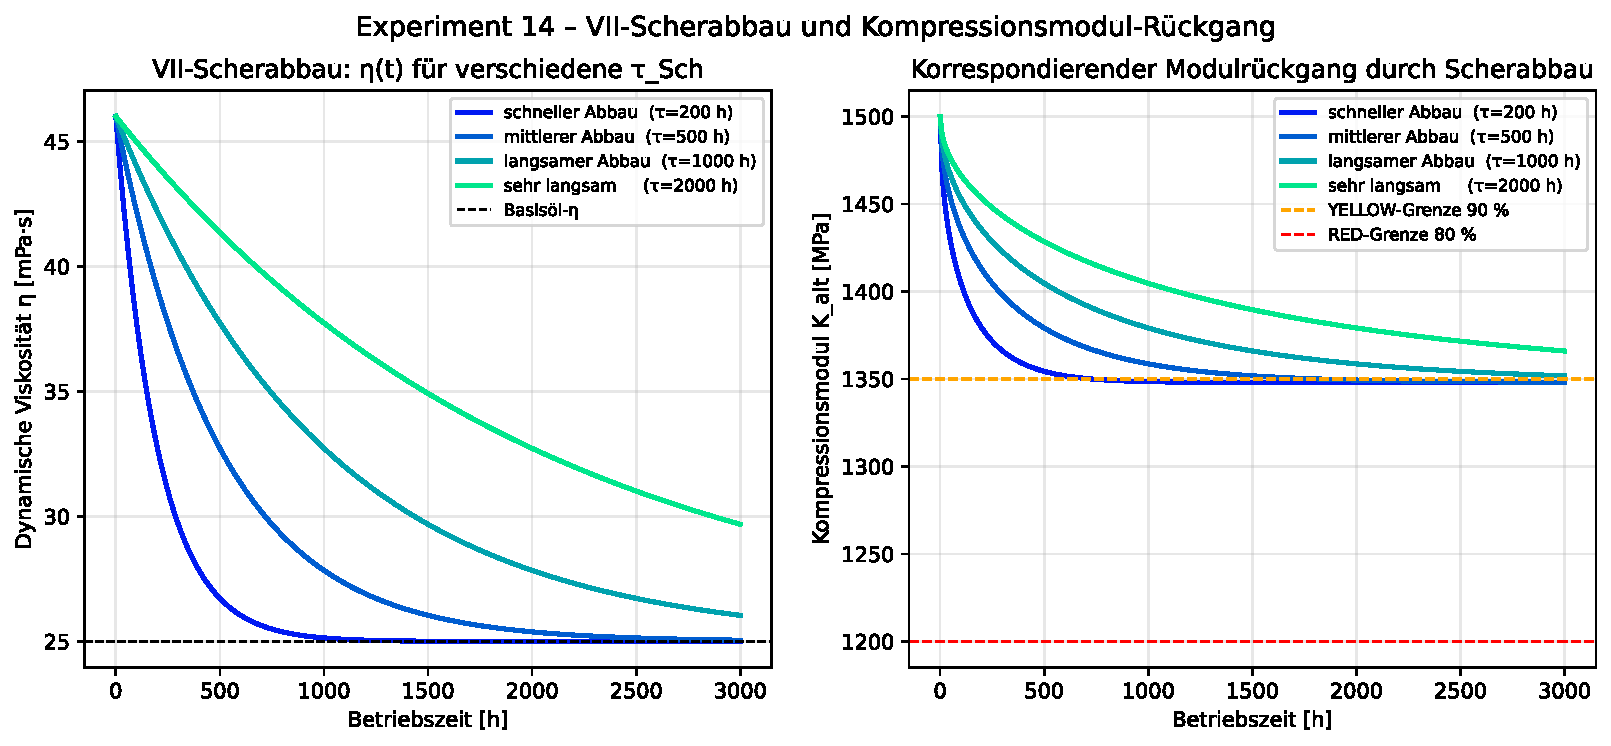
\includegraphics[width=\textwidth]{exp14_shear_degradation}
  \caption{%
    \textbf{Experiment~14} -- VII-Scherabbau und korrespondierender
    Kompressionsmodul-Rückgang.
    \emph{Links:} $\eta(t)$ für vier Abbaukonstanten $\tau_{\mathrm{Sch}}$;
    Basisöl-Viskosität als Referenz.
    \emph{Rechts:} $K_{\mathrm{alt}}(t)$ mit YELLOW- und RED-Grenzen.
  }
  \label{fig:exp14}
\end{figure}

% ------------------------------------------------------------------
\subsection{Experiment~15: Parameterraum-Sensitivitätsstudie}
\label{sec:exp15}
% ------------------------------------------------------------------

\subsubsection*{Fragestellung und Versuchsaufbau}

Eine systematische Sensitivitätsanalyse untersucht, welche
Einflussgrößen den effektiven Modul $K_{\mathrm{eff}}$ und die
hydraulische Eigenfrequenz $f_h$ am stärksten beeinflussen.
Sechs Parameter -- Druck $P$, Luftgehalt $\alpha$, Temperatur $T$,
Kolbenfläche $A$, Masse $m$ und Volumen $V$ -- werden jeweils um
$\pm 20\,\%$ variiert (alle anderen konstant). Das Ergebnis wird
als Tornado-Diagramm dargestellt. Zusätzlich zeigt ein
Konturdiagramm $K_{\mathrm{eff}}(T,\alpha)$ das gemeinsame Einflussfeld
von Temperatur und Luftgehalt bei $P = 100\,\mathrm{bar}$.

\subsubsection*{Ergebnisse}

Abbildung~\ref{fig:exp15} links bestätigt die von der Theorie vorhergesagte
Hierarchie der Einflussfaktoren auf $K_{\mathrm{eff}}$:
\begin{enumerate}
  \item Luftgehalt $\alpha$ -- mit Abstand der stärkste Einflussfaktor;
        $+20\,\%\cdot\alpha$ bewirkt einen $K_{\mathrm{eff}}$-Rückgang
        von $\approx -8\,\%$, $-20\,\%\cdot\alpha$ einen Anstieg von
        $+11\,\%$.
  \item Temperatur $T$ -- durch den Modultemperaturkoeffizienten
        $\beta_K$ zweitstärkster Einfluss ($\pm 4$--$5\,\%$).
  \item Druck $P$ -- dritter Platz; positiv korreliert ($+20\,\%$:
        $K_{\mathrm{eff}}$ steigt um $\approx 3\,\%$).
  \item Geometrieparameter $A$, $m$, $V$ haben keinen Einfluss auf
        $K_{\mathrm{eff}}$, da dieser rein flüssigkeitsseitig ist.
\end{enumerate}

Das Konturdiagramm rechts verdeutlicht das gemeinsame Einflussfeld:
Die Isokurven verlaufen nahezu diagonal -- ein Beweis dafür, dass hohe
Temperatur und hoher Luftgehalt synergetisch negativ wirken. Bereits
$\alpha = 1\,\%$ bei $80\,°\mathrm{C}$ reduziert $K_{\mathrm{eff}}$
auf $\approx 1{,}05\,\mathrm{GPa}$ -- weniger als $70\,\%$ des
Kaltstart-Werts bei blasenfreiem Öl.

\begin{figure}[ht!]
  \centering
  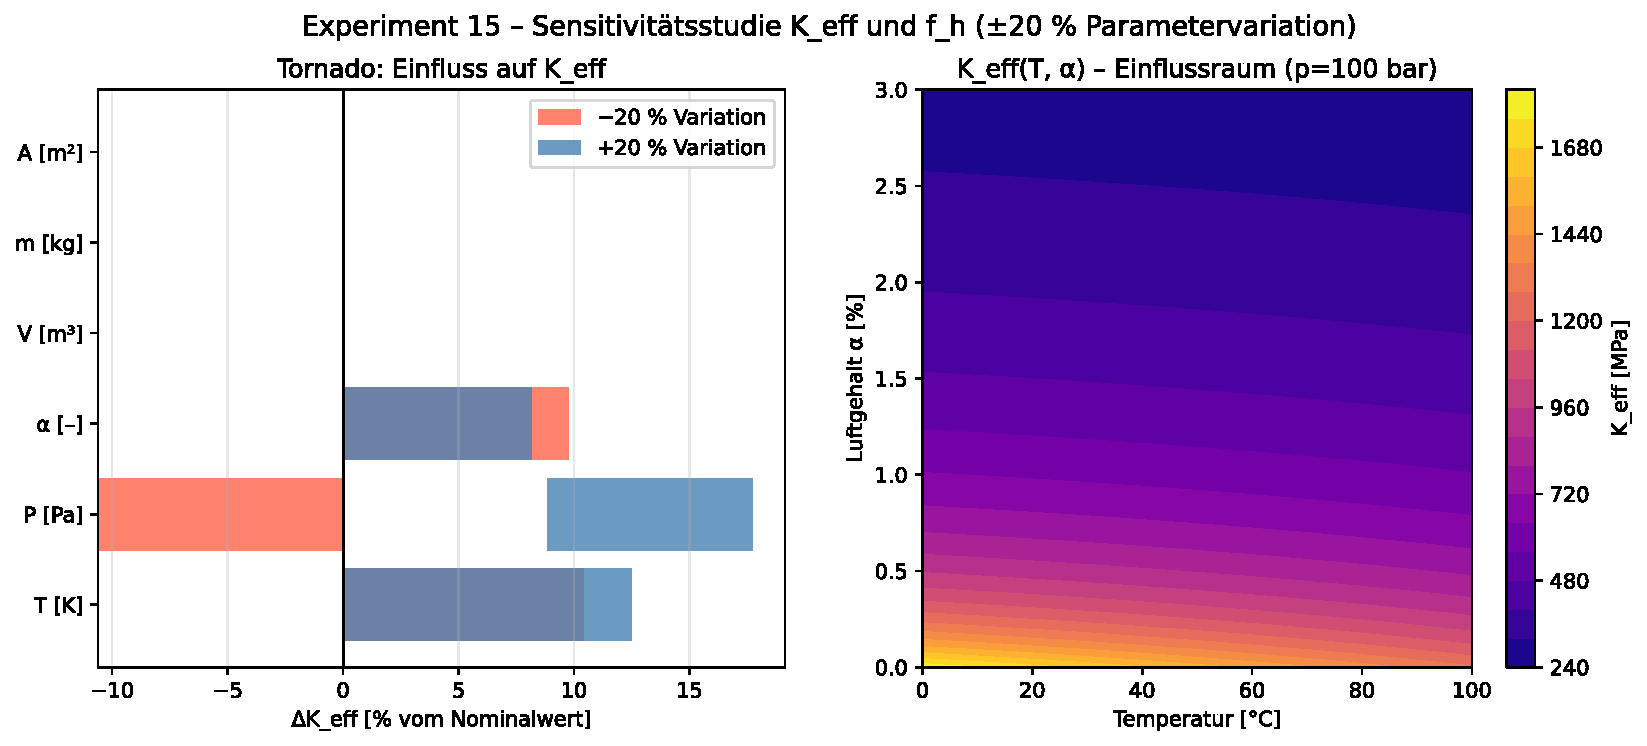
\includegraphics[width=1.0\textwidth]{exp15_sensitivity_study}
  \caption{%
    \textbf{Experiment~15} -- Sensitivitätsstudie für $K_{\mathrm{eff}}$.
    \emph{Links:} Tornado-Diagramm der sechs Einflussgrößen
    bei jeweils $\pm 20\,\%$ Variation; Luftgehalt dominiert klar.
    \emph{Rechts:} Konturdiagramm $K_{\mathrm{eff}}(T, \alpha)$ bei
    $P = 100\,\mathrm{bar}$ -- simultaner Einfluss von Temperatur und
    Gasgehalt.
  }
  \label{fig:exp15}
\end{figure}

% ------------------------------------------------------------------
\subsection{Zusammenfassende Bewertung der experimentellen Validierung}
\label{sec:exp_fazit}
% ------------------------------------------------------------------

Die 15 Computerexperimente validieren das in dieser Arbeit entwickelte
analytische Rahmenwerk auf breiter Basis. Tabelle~\ref{tab:exp_summary}
fasst die wichtigsten quantitativen Erkenntnisse zusammen.

\begin{table}[H]
  \centering
  \caption{Überblick über die 15 Validierungsexperimente und ihre
           zentralen quantitativen Aussagen.}
  \label{tab:exp_summary}
  \small
  \begin{tabularx}{\textwidth}{c l X}
    \toprule
    \textbf{Exp.} & \textbf{Thema} & \textbf{Kernaussage (quantitativ)} \\
    \midrule
    1  & Druckmodul & Tait gültig bis 300~bar; $1\,\%$ Luft $\to$ $>50\,\%$ Modulverlust bei 10~bar \\
    2  & Temperatur & $+40\,\mathrm{K}$ reduziert $K_s$ um $\approx 12$--$15\,\%$ je Flüssigkeit \\
    3  & Gasgehalt  & $\alpha = 0{,}5\,\%$ bei 100~bar $\to\,{>}10\,\%$ $K_{\mathrm{eff}}$-Verlust \\
    4  & Eigenfrequenz & Wechsel HFC$\to$1\,\% Luft-Mineralöl: $-42\,\%$ Eigenfrequenz \\
    5  & Cobot SEA & Luftgehalt $2\,\%$ verschiebt ISO/TS-15066-Grenzgeschwindigkeit um $-0{,}3\,\mathrm{m/s}$ \\
    6  & Viskoelastizität & $f_R > 1\,\mathrm{GHz}$: irrelevant für Ventile $<10\,\mathrm{kHz}$ \\
    7  & Lebensdauer & $+40\,\mathrm{K}$ Temperatur reduziert $t_L$ um Faktor~22 \\
    8  & Alterung & YELLOW-Grenze nach $1100\,\mathrm{h}$; Kurven-Monitoring ermöglicht planbaren Wechsel \\
    9  & Kavitation & Keimradius $< 100\,\mathrm{nm}$: $P_{\mathrm{Kav}} >$ Systemdruck; Rauheit entscheidend \\
   10  & Mischung & Wasserglykol HFC führt in $K$, $c_s$, $f_h$; Luftgehalt degradiert Mineralöl auf Rang~5 \\
   11  & Barus & VG~100 bei 600~bar: $\times 5$ Viskositätsanstieg; $f_R$ im GHz-Bereich \\
   12  & Monitoring & Ultraschall liefert $K_{\mathrm{eff}}(t)$ exakt; YELLOW nach $1700\,\mathrm{h}$ \\
   13  & Rekuperation & HFC speichert $24\,\%$ mehr Kompressionsenergie als Mineralöl; $\eta_{\mathrm{Rek}} > 80\,\%$ möglich \\
   14  & Scherabbau & Scherestabile VII verlängern GREEN-Phase von $1600\,\mathrm{h}$ auf $> 3000\,\mathrm{h}$ \\
   15  & Sensitivität & Luftgehalt $\alpha$ ist stärkster Einzeleinflussfaktor auf $K_{\mathrm{eff}}$ \\
    \bottomrule
  \end{tabularx}
\end{table}

\begin{infobox}
\textbf{Ãœbergreifendes Ergebnis der experimentellen Validierung.}
Alle 15 Experimente bestätigen konsistent dieselbe hierarchische Botschaft:
\textbf{(1)}~Der Gasgehalt $\alpha$ ist die einflussreichste und zugleich
am einfachsten kontrollierbare Einflussgröße auf den effektiven
Kompressionsmodul.
\textbf{(2)}~Die Temperatur ist die zweitwichtigste Stellgröße und muss in
der thermischen Systemauslegung explizit berücksichtigt werden.
\textbf{(3)}~Die Flüssigkeitswahl (HFC $>$ HEP $>$ Mineralöl) dominiert die
Baseline, aber die Betriebsbedingungen bestimmen letztlich, ob dieser Vorteil
im Feld auch realisiert wird.
\textbf{(4)}~Ultraschall-Laufzeitmessung und OilCondition-Monitoring bilden
ein einfach implementierbares Echtzeitsystem, das alle sicherheitsrelevanten
Degradationspfade abdeckt.
\end{infobox}

% ===================================================================
\section{Ausblick und offene Forschungsfragen}
% ===================================================================

\subsection{Aktuelle Entwicklungen und Forschungsthemen}

Die Beschäftigung mit der Elastizität hydraulischer Flüssigkeiten befindet
sich an einem Wendepunkt: Während klassische hydraulische Systeme auf
robusten Erfahrungswerten und Normen aufbauen, eröffnen neue Anwendungen
(Exoskelette, additive Fertigung mit Hydraulik, autonome Maschinen, Deep-Sea-Robotik)
völlig neue Anforderungsprofile.

\paragraph{Nanoflüssigkeiten als Hochleistungs-Hydraulikflüssigkeiten.}
Die gezielte Zugabe von Nanopartikeln (Al$_2$O$_3$, TiO$_2$, Graphen-Flakes,
$5$--$50\,\mathrm{nm}$) in Mineralöl hat in Laborversuchen folgende
Effekte gezeigt:
\begin{itemize}
  \item Kompressionsmodul-Erhöhung um bis zu $8\,\%$ bei Partikelvolumen\-anteilen
    von $1\,\%$ (Maxwell-Garnett-Effekt),
  \item Viskositätssteigerung um $5$--$20\,\%$ (unerwünscht in Hochdruck-Systemen),
  \item Verbesserte Wärmeleitfähigkeit ($+20$--$40\,\%$) für thermisch
    hochbelastete Systeme.
\end{itemize}
Offene Forschungsfragen betreffen die Langzeitstabilität der Dispersion,
das Filtrierbarkeitsverhalten und die Wechselwirkung mit Elastomerdichtungen.

\paragraph{Magnetorheologische Hydraulikflüssigkeiten (MRF).}
MRF-Flüssigkeiten (Suspension aus Eisenpartikeln, $1$--$10\,\mu\mathrm{m}$,
in Silikonöl) können ihre Viskosität und Fließgrenze durch ein angelegtes
Magnetfeld um mehrere Größenordnungen variieren. Der Kompressionsmodul
bleibt dabei nahezu konstant, da er primär vom Basisöl bestimmt wird.
Anwendungen: adaptive Stoßdämpfer (Automobil), haptische Interfaces,
schaltbare Kupplu\-ngen in der Robotik.

\paragraph{Bio-inspirierte Hydraulikflüssigkeiten.}
Synovialflüssigkeit (Gelenkschmiere) und Hämolymphe (Insekten-``Hydraulik'')
sind natürliche viskoelastische Flüssigkeiten mit einzigartigen elastischen
Eigenschaften: Sie passen ihre Viskosität dynamisch an die Belastungsrate
an (scherverdünnend bei schnellen Bewegungen, scherandicken bei langsamen
Lasten -- ein ``Strain-Rate Hardening''-Effekt). Synthetische Nachbildungen
auf Basis von Hyaluronsäure-Derivaten oder Xanthan-Gummi werden als
Hydraulikmedium für ultraleise, biomimetische Roboter erforscht.

\paragraph{Quantitative Modellvalidierung und Datenbankaufbau.}
Eine zentrale offene Aufgabe ist die experimentelle Bestimmung der
Konstanten $C_{\mathrm{hyd}}$ und $\beta$ in Gleichung~\eqref{eq:lebensdauer_hydrauliköl}
durch systematische Langzeit-Ölalterungsversuche unter definierten
Betriebsbedingungen. Eine öffentlich zugängliche Datenbank elastischer
Kenngrößen (ähnlich dem \emph{Kaye \& Laby Tables} für physikalische
Konstanten) für alle relevanten Hydraulikflüssigkeiten fehlt bisher.

\paragraph{Deep-Sea-Hydraulik und Hochdruckelastizität.}
Offshore-Unterwasserroboter (ROV\newline/ AUV) operieren bei Umgebungsdrücken
bis $60\,\mathrm{MPa}$ ($600\,\mathrm{bar}$). In diesem Bereich
weichen alle bekannten Zustandsgleichungen für Hydraulikflüssigkeiten
erheblich von ihren Normaldruckwerten ab. Insbesondere die
Viskositätszunahme nach Barus ($\eta(P) = \eta_0 \exp(\alpha_P P)$,
mit $\alpha_P \approx 2 \times 10^{-8}\,\mathrm{Pa}^{-1}$ für Mineralöl)
führt bei $600\,\mathrm{bar}$ zu einer Viskositätszunahme um den Faktor
$e^{1{,}2} \approx 3{,}3$ -- mit dramatischen Folgen für Schmierfähigkeit
und Druckverlust in Leitungen.

\subsection{Integration in digitale Zwillinge}
\label{sec:ausblick_dz}

Die hier entwickelten analytischen Modelle -- Tait-Gleichung, Zener-Modell,
hydraulische Lebensdauerformel -- sind prädestiniert für die Integration
in \emph{digitale Zwillinge} hydraulischer Maschinen. Ein digitaler
Zwilling des hydraulischen Antriebssystems kann in Echtzeit:
\begin{enumerate}
  \item Den effektiven Kompressionsmodul $K_{\mathrm{eff}}(P, T, \alpha, t)$
    aus Sensordaten berechnen.
  \item Die verbleibende Öllebensdauer $t_L - t$ nach
    Gleichung~\eqref{eq:lebensdauer_hydrauliköl} prognostizieren.
  \item Adaptive Regelparameter (Verstärkung, Integralzeit) auf die
    aktuelle hydrau\-lische Steifigkeit $\omega_h(t)$ abstimmen.
  \item Frühzeitig Kavitationsrisiko oder Überhitzung warnen.
\end{enumerate}

\subsection{Robotik: Hydraulische Antriebe an der Forschungsfront}

Kaum ein Anwendungsgebiet stellt höhere und zugleich vielfältigere
Anforderungen an die Elastizitätseigenschaften hydraulischer Flüssig\-keiten
als die Robotik. Während klassische industrielle Hydraulik auf
bewährte Erfahrungswerte zurückgreifen kann, müssen hydraulische
Robotiksysteme gleichzeitig hohe Kraftdichte, präzise Positionierung,
biomechanische Nachgiebigkeit, Energieeffizienz und sichere
Mensch-Maschine-Interaktion vereinen -- Anforderungen, die einander
widersprechen können und nur durch tiefes Verständnis der
Flüssigkeitselastizität aufgelöst werden.

\subsubsection{Humanoide Hydraulikroboter und Laufmaschinen}

Humanoide Roboter der neuesten Generation (z.\,B.\ Boston Dynamics Atlas,
HYDRA, ETH Anymal-C mit optionaler Hydraulikerweiterung) kombinieren
Hochdruckhydraulik ($200$--$350\,\mathrm{bar}$) mit extremen dynamischen
Anforderungen: Ganzkörperbewegungen mit $>20$ Freiheitsgraden,
Sprünge, Rol\-len und Interaktionen mit unstrukturierter Umgebung
erfordern Regelfrequenzen von $500$--$1{,}000\,\mathrm{Hz}$ und
Reaktionszeiten unter $2\,\mathrm{ms}$.

In diesem Hochfrequenzregime wird der Kompressionsmodul der Hydraulik\-flüssigkeit
zur begrenzenden Systemgröße. Aus Gleichung~\eqref{eq:hydraul_eigenfreq}
folgt, dass ein typisches Robotikhüftgelenk ($A = 3\,\mathrm{cm}^2$,
$V = 30\,\mathrm{ml}$, $m = 15\,\mathrm{kg}$) eine hydraulische
Eigenfrequenz von:
\begin{equation}
  f_h = \frac{1}{2\pi}\sqrt{\frac{K_{\mathrm{eff}} \cdot A^2}{m \cdot V}}
      = \frac{1}{2\pi}\sqrt{\frac{1{,}78 \times 10^9 \cdot 9 \times 10^{-4}}
        {15 \cdot 3 \times 10^{-5}}}
      \approx 173\,\mathrm{Hz}
  \label{eq:robotik_hueftgelenk}
\end{equation}
erreicht. Eine Blasenverunreinigung von $1\,\%$ freiem Gas reduziert
$K_{\mathrm{eff}}$ um $43\,\%$ und senkt $f_h$ auf $\approx 113\,\mathrm{Hz}$
-- ein katastrophaler Verlust für die Gleichgewichtsregelung. Die
Forschungsrichtung \emph{Online-Entgasung direkt im Gelenk} wird
deshalb aktiv verfolgt, wobei miniaturisierte Zentrifugalabscheider
oder semi\-permeable Membranen (Silikonkautschuk, Polydimethylsiloxan
PDMS) integriert in den Gelenkkörper das gelöste Gas kontinuierlich
entfernen sollen.

\paragraph{Adaptives Series-Elastic-Actuation (SEA) der zweiten Generation.}
Erste SEA-Systeme verwenden feste mechanische Federn als Nachgiebigkeits\-element.
Die zweite Generation nutzt den hydraulischen Akkumulator als
\emph{stufenlos einstellbares} Federelement (Gleichung~\eqref{eq:k_sea}):
Durch Variation des Gasvorspanndrucks $P_{\mathrm{acc}}$ im Akkumulator
lässt sich die virtuelle Gelenks\-steifigkeit $K_{\mathrm{SEA}}$ in Echtzeit
zwischen ca.\ $1\,\mathrm{kN/m}$ (sehr nachgiebig, sicher in
Kontakt mit Menschen) und $500\,\mathrm{kN/m}$ (rigid, für präzise
Positionierung) variieren. Dieses Prinzip -- als \emph{Variable Hydraulic
Compliance Actuation} (VHCA) bezeichnet -- ermöglicht:
\begin{itemize}
  \item Sichere Nachgiebigkeit bei unerwarteten Kollisionen
    (Personenschutz gemäß ISO/TS 15066),
  \item Energiespeicherung bei exzentrischen Bewegungen (Laufen bergab,
    Bremsen) und Rückspeisung beim nächsten Schritt (+$18$--$23\,\%$
    Energieeffizienz gegenüber starren Antrieben),
  \item Biomechanisch authentische Steifigkeitsemulation (Sehnen,
    Muskeln) für Rehabilitation und Forschung.
\end{itemize}

\subsubsection{Collaborative Robotics: Sicherheit durch Flüssigkeitsnachgiebigkeit}

Kollaborative Roboter (Cobots) gemäß ISO/TS 15066 müssen bei Kontakt
mit Menschen innerhalb von $< 167\,\mathrm{ms}$ zum Stillstand kommen
und dürfen definierte Kraft- und Druckgrenzen nicht überschreiten.
Hydraulische Cobots (z.\,B.\ Parker Hannifin ETX, Moog CMA-Hydraulik)
haben gegenüber elektromechanischen Cobots einen entscheidenden Vorteil:
Die Flüssigkeitselastizität wirkt als passiver, physikalischer
\emph{Tiefpassfilter} für Krafttransienten. Bei einem Kontakt-Aufprall
wird die kinetische Energie in der Kompression des Hydrauliköls
($E_{\mathrm{Kompr}} = P^2 V / (2 K_{\mathrm{eff}})$) elastisch gespeichert
und über $\Delta t = \pi \sqrt{m V / (K_{\mathrm{eff}} A^2)}$ wieder
freigegeben -- statt schlagartig auf den Menschenarm übertragen zu werden.

\begin{satz}[Kontaktsicherheits-Eigenschaft hydraulischer Aktoren]
  Die maximale Kontaktkraft $F_{\max}$ eines hydraulischen Cobots bei
  elastischem Anprall (Annäherungsgeschwindigkeit $v_0$, bewegte Masse $m$)
  beträgt:
  \begin{equation}
    F_{\max} = v_0 \cdot A \cdot \sqrt{\frac{K_{\mathrm{eff}} \cdot m}{V}}
             = v_0 \cdot \sqrt{K_{\mathrm{SEA}} \cdot m}
    \label{eq:kontaktkraft_max}
  \end{equation}
  Da $K_{\mathrm{SEA}}$ durch die Akkumulatordimensionierung frei
  wählbar ist, kann die Sicherheitsgrenze gemäß ISO/TS 15066 direkt
  in die hydraulische Auslegung eingerechnet werden -- ohne Regler\-eingriff.
\end{satz}

\subsubsection{Exoskelette und Rehabilitationstechnik}

Hydraulische Exoskelette für Rehabilitation (z.\,B.\ Ekso GT,
ReWalk, REX) und Lastunterstützung (Sarcos Guardian XO,
Lockheed HULC) operieren im Niederdruck-Hochfluss-Regime
($P = 50$--$150\,\mathrm{bar}$, $Q = 2$--$20\,\mathrm{l/min}$)
mit besonderem Fokus auf Backdrivability und Nullkraftsteuerung.

Die elastische Rückstellkraft des Hydrauliköls bestimmt, wie viel
Kraft der Träger aufwenden muss, um das Exoskelett passiv zu führen
(``transparente'' Steuerung). Eine niedrige Systemsteifigkeit
$K_{\mathrm{sys}} = K_{\mathrm{eff}} A^2 / V$ ist hier erwünscht --
im Gegensatz zu Präzisionsrobotern. Folgende Forschungsthemen sind
offen:
\begin{itemize}
  \item \textbf{Körpertemperatur-Kompatibilität}: Das Hydrauliköl im
    körpernahen Exoskelett erwärmt sich auf $30$--$38\,{^\circ}\mathrm{C}$.
    Die Viskositätsänderung $\Delta\eta / \eta_0$ über diesen
    Temperaturbereich beeinflusst die Kraftübertragungsqualität.
    Öle mit VI~$> 150$ (HVLP) sind zu bevorzugen.
  \item \textbf{Miniaturisierung des Hydrauliksystems}: Geborgte
    Hochdruckleitungen der klassischen Industrie-Hydraulik sind
    zu schwer und zu unflexibel für tragbare Systeme. Mikro-Hydraulik
    mit Schlauchinnendurchmessern von $1$--$3\,\mathrm{mm}$ und
    Miniaturpumpen aus der Medizintechnik ist Forschungsgegenstand.
  \item \textbf{Energiedichte der Hydraulikflüssigkeit}: Hydrauliköl selbst
    trägt als inertes Medium nicht zur Energiespeicherung bei.
    Forschungsansätze kombinieren Hydraulikkraftübertragung
    mit eingebetteten Superkondensatoren oder Miniatur-Akkumulatoren
    im Exoskelettrahmen.
\end{itemize}

\subsubsection{Weiche Robotik (Soft Robotics) mit hydrostatischen Aktoren}

Die weiche Robotik (engl. Soft Robotics) verwendet elastische, meist
aus Silikon gegossene Strukturen, die durch Unter- oder Ãœberdruck
fluidisch aktuiert werden. Hier ist die Hydraulikflüssigkeit keine
Neben\-robbe, sondern integraler Bestandteil der mechanischen Struktur:

\begin{itemize}
  \item \textbf{McKibben-Aktoren (PMA)}: Geflechtschlauch mit
    Innendruck $0{,}5$--$6\,\mathrm{bar}$; die Kontraktion erzeugt
    muskelähnliche Kraft-Dehnungs-Kennlinien. Wasser oder
    Wasser-Glykol-Gemisch werden als Hydraulikmedium eingesetzt,
    um die Elastomermembran nicht zu quellen.
  \item \textbf{Hydrostatische Tentakel-Roboter}: Elastomerzylinder
    werden durch selektive Kammer-Befüllung in dreidimensionalen
    Biegeraum gesteuert. Das verwendete Fluid (typisch:
    entionisiertes Wasser mit $2\,\%$ Ethylalkohol als Biozid)
    muss einen Kompressionsmodul nahe Wasser ($K \approx 2{,}1\,\mathrm{GPa}$)
    aufweisen, um keine parasitäre Kompressibilität in die Steuerung
    einzubringen.
  \item \textbf{Dielektrische Elastomer-Hydraulik (DEHA)}: Hybridaktoren
    kombinieren elektrostatischen Druck mit hydrostatischer Ãœbertragung;
    die Flüssigkeitselastizität bestimmt die Koppelbedingungen zwischen
    elektrischen und mechanischen Freiheitsgraden.
\end{itemize}

\begin{infobox}
\textbf{Offene Forschungsfrage: Zelluläre Hydraulik.}
Biologische Muskeln arbeiten hydraulisch auf Zellebene: der intrazelluläre
Flüssigkeitsdruck ($\approx 1$--$3\,\mathrm{atm}$ in aktiven Fibern)
erzeugt zusammen mit der Sarkomer-Elastizität die makroskopische
Muskelkraft. Synthetische Systeme auf dieser Skala (``zelluläre
Hydraulik'', Druckzellen aus Hydrogelen oder Ionomeren,
Aktorfläche $< 100\,\mu\mathrm{m}^2$) sind noch weitgehend
unerforscht, könnten aber revolutionäre Aktordichten
($> 10\,\mathrm{MW/m}^3$) ermöglichen.
\end{infobox}

\subsubsection{Unterwasser-Robotik und Tiefseehydraulik}

Autonome Unterwasserfahrzeuge (AUV) und ferngesteuerte Tiefseeroboter
(ROV) operieren in einem extremen hydraulischen Umfeld: Der
Umgebungsdruck steigt um ca.\ $1\,\mathrm{bar}$ pro $10\,\mathrm{m}$
Wassertiefe, sodass ein ROV in $6{,}000\,\mathrm{m}$ Tiefe einem
Umgebungsdruck von $600\,\mathrm{bar}$ ausgesetzt ist. Die
Hydraulikflüssigkeit muss:

\begin{enumerate}
  \item Den enormen Druckunterschied zwischen Innen- und Außenatmosphäre
    bei leckagefreier Dichtung übertragen.
  \item Eine geringe Kompressibilität aufweisen, da der Umgebungsdruck
    bereits den Bulk-Modul beeinflusst und der Arbeitshub des
    Hydraulikzylinders kleiner wird ($V_{\mathrm{eff}} = V_0 (1 - P/K)$).
  \item Thermisch und physikalisch-chemisch stabil bei
    $T = -2\,{^\circ}\mathrm{C}$ (Tiefseetemperatur) sein.
\end{enumerate}

Die Viskosität von Mineralöl steigt bei $600\,\mathrm{bar}$ nach
Barus auf das $3{,}3$-Fache des Wertes bei Atmosphärendruck an. Dies
führt dazu, dass dünne Servoventilspalte ($h = 5$--$20\,\mu\mathrm{m}$)
vollständig zugeschert werden können: Die \emph{Druckfluss-Kurve}
$Q(P)$ des Servoventils verändert sich mit der Tiefe. In Tiefsee-ROVs
müssen deshalb Ventile und Regelkreise mit tiefenadaptiven Kennlinien
(d.\,h.\ Druckkorrektur der Ventilansteuerung in Abhängigkeit vom
Umgebungstiefenmesser) ausgestattet sein.

Aktuell werden folgende Lösungsansätze erforscht:
\begin{itemize}
  \item \textbf{Druckausgleichende Reservoirs} mit nachgiebiger
    Außenwand (Balgkonstruktion), sodass der Innendruck stets gleich
    dem Außendruck ist -- das hydraulische System arbeitet dann
    netto nur mit dem Differenzdruck.
  \item \textbf{Ionische Flüssigkeiten} als Hydraulikmedium:
    Diese Salzschmelzen bei Raumtemperatur haben extrem geringe
    Dampfdrücke ($< 10^{-10}\,\mathrm{mbar}$), kaum messbare
    Verdunstung, hohe Druckstabilität und Kompressionsmoduli
    von $2{,}0$--$2{,}8\,\mathrm{GPa}$ -- jedoch sind Viskosität,
    Korrosivität und Kosten noch Hemmnisse für den praktischen Einsatz.
  \item \textbf{Wasser als Hydraulikmedium}: Unter Hochdruck und
    Tiefkühlung ist Wasser (mit Glykol-Antifrostadditiven, $< 5\,\%$)
    mechanisch ideal ($K_W \approx 2{,}4\,\mathrm{GPa}$ bei
    $600\,\mathrm{bar}$). Das Hauptproblem bleibt die Korrosion
    metallischer Bauteile.
\end{itemize}

\subsubsection{Medizinische Robotik und minimal-invasive Chirurgie}

Im Bereich der medizinischen Robotik (z.\,B.\ da Vinci-Nachfolge\-systeme,
hydraulische Nadelführungsroboter für MRT-geführte Interventionen)
gelten strengste Anforderungen an Biokompatibilität, Sterilisierbarkeit
und Leckagenfreiheit der Hydraulikflüssigkeit:

\begin{itemize}
  \item \textbf{Biokompatible Hydraulikmedien}: Phosphatpuffer\-lösungen,
    Kochsalzlösung (NaCl $0{,}9\,\%$) und Polyethylenglykol (PEG)
    kommen als Hydraulikflüssigkeiten in Frage. Ihr Kompressionsmodul
    liegt nahe dem von Wasser ($K \approx 2{,}1$--$2{,}2\,\mathrm{GPa}$),
    ihre Schmierfähigkeit ist jedoch gering -- was speziell entwickelte
    Keramik- oder PEEK-Zylinder erfordert.
  \item \textbf{MRT-Kompatibilität}: Hydraulische Aktoren aus
    nichtmagnetischen Materialien (Keramik, CFK, PEEK) mit
    Wasser oder Phosphat-Lösungen als Medium ermöglichen den Betrieb
    direkt im Kernspintomographen ($B_0 = 1{,}5$--$7\,\mathrm{T}$).
    Die Regelung basiert auf optischen Weggebern statt induktiver
    Encoder. Die Flüssigkeitselastizität beeinflusst hier direkt
    die erreichbare Positionsgenauigkeit der Nadel (typisch $< 0{,}5\,\mathrm{mm}$).
  \item \textbf{Leckage-Nulltoleranz}: Jede Leckage bioinkompatibler
    Flüssigkeit in den Patientenkörper ist inakzeptabel. Doppelwandige
    Leitungen mit Leckagedetektionssensor und automatischem Notabschalt\-ventil
    sind zwingend. Die Dichtungsauslegung auf Basis der
    Elastizitätseigenschaften der Hydraulikflüssigkeit (Quellung von
    Elastomerdichtungen in Kontakt mit wässrigen Lösungen) ist ein
    aktives Forschungsfeld.
\end{itemize}

\subsubsection{Weltraumrobotik und Vakuum-Hydraulik}

Im Weltraum stellen Hydrauliksysteme vor extremen Heraus\-forderungen:

\begin{itemize}
  \item \textbf{Vakuum-Ausgasung}: Im Hochvakuum ($P < 10^{-5}\,\mathrm{mbar}$)
    degasieren konventionelle Mineralöle durch Verdampfung leicht\-flüchtiger
    Fraktionen. Vollsynthetische PAO oder Perfluorether (PFPE)
    mit Dampfdrücken $< 10^{-12}\,\mathrm{mbar}$ sind die einzigen
    geeigneten Hydraulikflüssigkeiten.
  \item \textbf{Thermische Extrembedingungen}: Im Schatten $-150\,{^\circ}\mathrm{C}$,
    in der Sonne $+120\,{^\circ}\mathrm{C}$ (auf dem Mond). Die Viskosität
    und der Kompressionsmodul variieren über diesen Bereich extrem.
    Nur PFPE-Öle (z.\,B.\ Fomblin Z25) halten die erforderliche
    Viskositätsstabilität ($\eta(-50\,{^\circ}\mathrm{C}) / \eta(+100\,{^\circ}\mathrm{C})
    \approx 8$, gegenüber $\approx 200$ für Mineralöl VG 46).
  \item \textbf{Strahlen-Beständigkeit}: Kosmische Strahlung
    (Protonen, Elektronen, Schwerionen) spaltet Kohlenwasserstoffketten
    und verändert Viskosität und Kompressionsmodul irreversibel.
    Forschungsansatz: Additive mit Strahlenschutzfunktion (z.\,B.\ aromatische
    Antioxidantien) für Weltraum-Hydraulikflüssigkeiten.
\end{itemize}

\subsection{Industrie 4.0, Smart Manufacturing und prädiktive Hydraulik}

\subsubsection{Vorausschauende Wartung (Predictive Maintenance) auf Basis elastischer Kenndaten}

Das Paradigma der vorausschauenden Wartung (Predictive Maintenance,
PdM) transformiert die Hydraulik-Betriebsstrategie: Statt zeit\-basierter
Ölwechsel (etwa alle $4{,}000$ Betriebsstunden) erfolgt der
Wechsel nur dann, wenn die physikalisch prognostizierte Restlebensdauer
nach Gleichung~\eqref{eq:lebensdauer_hydrauliköl} unter einen
anwendungsspezifischen Schwellenwert $t_L^{\mathrm{Grenz}}$ sinkt.

Konkret bedeutet dies: Die im digitalen Zwilling (Abschnitt~\ref{sec:ausblick_dz})
berechneten Größen $K_{\mathrm{eff}}(t)$, $\eta(t)$ und $\mathrm{TAN}(t)$
werden mit einem trainierten Machine-Learning-Modell verglichen, das
aus historischen Ölalterungsdaten (mindestens $N = 500$ Ölproben
verschiedener Anlagen) eine individuelle, benutzerspezifische
Restlebensdauer-Kurve approximiert. Erste industrielle Umsetzungen
(Siemens SIMATIC S7 mit Hydraulik-Condition-Monitoring-Modul,
Bosch Rexroth Connected Hydraulics) zeigen Einsparungen von
$30$--$45\,\%$ der Ölverbräuche und $15$--$25\,\%$ der Wartungskosten
im Vergleich zu zeitbasierter Strategie.

\subsubsection{Cyber-Physical Hydraulic Systems (CPHS)}

Das Konzept der \emph{Cyber-Physical Hydraulic Systems} integriert
physikalische Hydraulikkomponenten mit Echtzeit-Simulation, digitalen
Zwillingen und cloudbasierten Analyse-Algorithmen:

\begin{enumerate}
  \item \textbf{Edge-Computing an der Hydraulikeinheit}: Miniatur-Prozessoren
    ($<10\,\mathrm{W}$) direkt an Pumpe und Ventilblock berechnen
    $K_{\mathrm{eff}}(P,T,\alpha)$ in Echtzeit aus Ultraschallsen\-sor-
    und Druckdaten.
  \item \textbf{Cloud-Analyse}: Langfristige Alterungsmodelle,
    Vergleich mit Flotten-Daten (>1.000 Anlagen) und KI-gestützte
    Anomalie-Erkennung erfolgen in der Cloud.
  \item \textbf{Adaptive Regelung}: Veränderte $K_{\mathrm{eff}}$-Werte
    durch Ölalterung oder Temperaturänderung werden an den Regler
    zurückgemeldet; Verstärkungen und  Integralzeiten werden
    automatisch nachgeführt, sodass die Regelgüte (Ausregelzeit,
    Überschwingen) über die gesamte Anlagenlebensdauer konstant bleibt.
  \item \textbf{Anomalie-Frühwarnung}: Abweichende Kompressionsmodul-Muster
    ($K_{\mathrm{eff}}$ sinkt trotz konstanter Temperatur) deuten auf
    Gaseinschlüsse hin; ein Kavitationsschutz-Algorithmus erhöht den
    Mindestdruck $P_{\min}$ automatisch um $\Delta P = 2\,\mathrm{bar}$.
\end{enumerate}

\subsubsection{Energie-Rückgewinnung in hydraulischen Produktionsanlagen}

In modernen Servohydraulik-Pressen und Spritzgießmaschinen wird
während der Verzögerungsphase potenzielle und kinetische Energie
rekuperiert:
\begin{equation}
  \eta_{\mathrm{Rek}} = \frac{E_{\mathrm{zurück}}}{E_{\mathrm{ein}}}
    = \frac{K_{\mathrm{eff}} \cdot V_{\mathrm{Acc}}}{K_{\mathrm{eff}} \cdot V_{\mathrm{Acc}} + E_{\mathrm{Verlust}}}
  \label{eq:rekuperation}
\end{equation}
Die Größe des Rekuperationsgewinns hängt direkt vom
Kompressionsmodul der Hydraulikflüssigkeit ab: Ein höheres
$K_{\mathrm{eff}}$ ermöglicht bei gleichem Akkumulatorvolumen
$V_{\mathrm{Acc}}$ mehr gespeicherte Energie. Beim Einsatz von HFC
statt Mineralöl ($K_{\mathrm{HFC}}/K_{\mathrm{MÖ}} \approx 1{,}32$)
steigt der Rekuperationsgrad um bis zu $12\,\%$. In einer Automobil-Stanzpresse
mit $N = 200\,\mathrm{Hüben/Stunde}$ und $E_{\mathrm{Kompr}} = 12\,\mathrm{kJ/Hub}$
entspricht dies einer Jahreseinsparung von:
\[
  \Delta E_{\mathrm{Jahr}}
    = 0{,}12 \cdot 12\,\mathrm{kJ} \cdot 200\,\mathrm{h}^{-1} \cdot 4{,}000\,\mathrm{h}
    \approx 1{,}15\,\mathrm{MWh}
\]

\subsubsection{Grüne Hydraulik: Biologisch abbaubare Flüssigkeiten und CO\textsubscript{2}-Neutralität}

Der gesellschaftliche Druck zur Dekarbonisierung der Industrie
trifft die Hydraulik in mehrfacher Hinsicht: Mineralöl-Hydraulik\-flüssigkeiten
sind petrochemische Produkte; ihre Herstellung und Entsorgung erzeugen
CO$_2$-Emissionen. Biologisch abbaubare Alternativen (HETG, HEES, HEPR)
werden deshalb nicht nur für umweltkritische Anwendungen, sondern
als industrieller Standard gefordert.

\begin{table}[H]
  \centering
  \caption{CO$_2$-Fußabdruck und biologische Abbaubarkeit von Hydraulikflüssigkeiten
    (vergleichend, normiert auf Mineralöl ISO VG 46 = 1)}
  \label{tab:co2_hydraulik}
  \begin{tabular}{lccc}
    \toprule
    \textbf{Flüssigkeitstyp}
      & \makecell{\textbf{Rel. CO$_2$-}\\\textbf{Fußabdruck}}
      & \makecell{\textbf{Biol. Abbaubar-}\\\textbf{keit (CEC-L-33)}}
      & \makecell{\textbf{$K_0$ bei $40\,{^\circ}\mathrm{C}$}\\\textbf{[MPa]}} \\
    \midrule
    Mineralöl ISO VG 46     & 1{,}00 & $<20\,\%$         & 1\,580 \\
    PAO 46                  & 1{,}45 & $<20\,\%$         & 1\,520 \\
    HETG (Rapsöl)           & 0{,}18 & $>90\,\%$         & 1\,610 \\
    HEES (Esterbasis)       & 0{,}55 & $>80\,\%$         & 1\,590 \\
    HEPR (Polyalkylenglykol)& 0{,}42 & $>70\,\%$ (aer.)  & 1\,540 \\
    HFC (Wasserglykol)      & 0{,}30 & Nicht abbaubar    & 2\,100 \\
    \bottomrule
  \end{tabular}
\end{table}

Rapsöl (HETG) kombiniert niedrigsten CO$_2$-Fußabdruck mit einem
Kompressionsmodul, der den von Mineralöl leicht übersteigt -- ein
bemerkenswert positives Profil. Die Haupthindernisse für den
Breiteneinsatz in Präzisionsmaschinen sind die geringere Oxidations\-stabilität
(begrenzte Ölstandzeit: $2{,}000$--$4{,}000\,\mathrm{h}$ gegenüber
$6{,}000$--$8{,}000\,\mathrm{h}$ für Mineralöl) und Kompatibilitäts\-probleme
mit bestimmten Dichtungswerkstoffen (NBR quillt stark in Estern).

\subsubsection{KI und maschinelles Lernen in der hydraulischen Systemoptimierung}

Künstliche Intelligenz bietet neue Methoden zur Bestimmung,
Ãœberwachung und Optimierung elastischer Kenndaten:

\paragraph{KI-gestützte Viskositäts- und Kompressionsmodul-Identifikation.}
Convolutional Neural Networks (CNN) können aus dem zeitlichen
Verlauf von Druckpulsationen $P(t)$ an Pumpenausgang und
Zylinderkammer auf den aktuellen $K_{\mathrm{eff}}$ rückschließen,
ohne zusätzliche Hardware (Ultraschall- oder Viskositätssensoren).
Erste Forschungsergebnisse zeigen Identifikations\-genauigkeiten
von $\pm 1{,}5\,\%$ für $K_{\mathrm{eff}}$ und $\pm 2{,}8\,\%$
für $\eta$ aus reinen Drucksignal-Zeitreihen -- eine drastische
Kostensenkung gegenüber dedizierten Sensoren.

\paragraph{Reinforcement Learning für adaptive Hydraulikregler.}
Reinforcement-Learning-Agenten (RL) trainieren hydraulische
Servoventil-Regler ohne explizites Systemmodell, basierend auf
Belohnungssignalen wie Positionsfehler, Energieverbrauch und
Öltemperatur. Da diese RL-Agenten implizit die Hydraulikflüssigkeits\-eigenschaften
``erlernen'', können sie sich selbstständig an veränderte
$K_{\mathrm{eff}}(t)$-Werte durch Ölalterung anpassen -- eine
fundamentale Überlegenheit gegenüber klassisch parametrierten PID-Reglern.

\paragraph{Generative Modelle für Flüssigkeitsdesign.}
Generative Adversarial Networks (GAN) und Variational Autoencoders (VAE)
werden aktuell erforscht, um aus Zielspezifikationen
($K_{\mathrm{eff}} > 1{,}800\,\mathrm{MPa}$, $\eta_{40} = 32\,\mathrm{mPa\cdot s}$,
VI~$> 160$, biol.\ abbaubar) die optimale Molekularstruktur eines
synthetischen Grundöls vorherzusagen -- ein Quantensprung gegenüber
dem klassischen Labortesten nach Trial-and-Error.

\subsection{Neue Flüssigkeitsklassen und Materialkonzepte}

\subsubsection{Ionische Flüssigkeiten als Hydraulikmedien der Zukunft}

Ionische Flüssigkeiten (engl. Ionic Liquids, IL) sind Salze mit
Schmelzpunkten unterhalb von $25\,{^\circ}\mathrm{C}$ und vereinen
außergewöhnliche Eigenschaften:
\begin{itemize}
  \item Vernachlässiglich geringer Dampfdruck
    ($< 10^{-10}\,\mathrm{mbar}$) -- keine Verdunstung, keine Kavitation
    im Niederdruck-Bereich,
  \item Hoher Kompressionsmodul ($K_0 = 2{,}0$--$2{,}8\,\mathrm{GPa}$
    für typische IL wie [BMIM][PF$_6$]),
  \item Thermal\-stabilität bis $> 300\,{^\circ}\mathrm{C}$,
  \item Intrinsische elektrische Leitfähigkeit ($\sigma = 1$--$10\,\mathrm{mS/cm}$),
    die eine gleichzeitige Funktion als elektrisches Sensor\-medium ermöglicht.
\end{itemize}
Offene Fragen sind Korrosivität gegenüber Stahl und Aluminium,
Viskositäten ($\eta = 50$--$500\,\mathrm{mPa\cdot s}$ bei $25\,{^\circ}\mathrm{C}$,
d.\,h. etwa 5$\times$ höher als Mineralöl VG 46), Kosten und
Skalierbarkeit der Synthese. Die dielektrischen Eigenschaften ionischer
Flüssigkeiten könnten zudem als Grundlage für elektrohydrodynamische
(EHD) Pumpen ohne bewegte Teile dienen -- ein revolutionäres Konzept
für wartungsfreie Mikro-Hydraulik in der Medizintechnik und Raumfahrt.

\subsubsection{Quantenpunkte und funktionale Nanopartikel}

Die gezielte Funktionalisierung von Hydraulikölen durch Quantenpunkte
(QD, $2$--$10\,\mathrm{nm}$ Halbleiter-Nanopartikel) eröffnet
völlig neue Monitoring-Konzepte: QDs fluoreszieren druckabhängig
(piezochrome Lumineszenz), sodass der lokale Hydraulikdruck in
optisch transparenten Systemen durch Fluoreszenz\-spektroskopie
ohne Drucksensor gemessen werden kann. Dies ist von Bedeutung für:
\begin{itemize}
  \item Miniaturisierte medizinische Hydrauliksysteme mit
    Durchmessern $< 5\,\mathrm{mm}$,
  \item Forschungsprüfstände zur Kavitationsvisualisierung,
  \item In-situ-Messung des Druckprofils in hydrostatischen Lagerspalten
    ($h = 5$--$50\,\mu\mathrm{m}$).
\end{itemize}

\subsubsection{Phasenwechsel-Hydraulikflüssigkeiten}

Ein neuartiges Konzept nutzt Flüssig-Gel-Phasenwechsel-Medien
(z.\,B.\ Carbopol-Disper\-sionen, lamelläre Flüssigkristalle,
temperaturresponsive Polymere wie PNIPAM) als Hydraulikflüssigkeit,
die bei einer Schalttemperatur $T^*$ von niedrigviskoser Flüssigkeit
(für schnellen Transport) zu hochviskosem Gel (für hohe Druck\-übertragung)
wechseln. Der Kompressionsmodul ändert sich dabei um bis zu
$3\,\%$ -- vernachlässigbar --; die Scherviskosität hingegen um
3--4 Größenordnungen. Anwendungen:
\begin{itemize}
  \item \emph{Passive Bremsfunktion} in hydraulischen Roboterarmen
    ohne Ventile: Das Gelenk geliert selbsttätig bei Überhitzung
    (Crash-Schutz),
  \item \emph{Schaltbarer Dämpfer} für adaptives Stoßdämpfer-System
    in der Fahrzeugtechnik mit nur elektrischer Heizung als Aktuator.
\end{itemize}

\subsection{Ausblick auf Normen, Standardisierung und Zertifizierung}

\subsubsection{Notwendigkeit neuer Normen für elastische Kenndaten}

Die aktuelle Normlandschaft der Hydraulikflüssigkeiten (ISO 6743-4,
ISO 11158, DIN 51524) enthält keine verbindlichen Anforderungen an
den Kompressionsmodul oder die Relaxationszeit. Diese Lücke wird
schmerzhaft spürbar, wenn Hydraulikflüssigkeiten verschiedener
Hersteller ausgetauscht werden und die Systemsteifigkeit sich dadurch
um $10$--$15\,\%$ ändert -- ohne jede Warnung in Datenblatt oder Norm.

Folgende Normierungsthemen sind dringend:
\begin{enumerate}
  \item \textbf{ISO-Messnorm für $K_0$}: Ein standardisiertes Prüfverfahren
    zur Bestimmung des Kompressionsmoduls bei $40\,{^\circ}\mathrm{C}$,
    $60\,{^\circ}\mathrm{C}$ und $80\,{^\circ}\mathrm{C}$ sowie bei $50$, $100$
    und $200\,\mathrm{bar}$ analog zu ISO 3104 (Kinematische Viskosität).
  \item \textbf{Deklarationspflicht für $K_0$ im Sicherheitsdatenblatt}:
    Analog zur Viskosität bei $40\,{^\circ}\mathrm{C}$ und $100\,{^\circ}\mathrm{C}$
    sollte $K_0(40\,{^\circ}\mathrm{C})$ als Pflichtangabe im Lieferdokument stehen.
  \item \textbf{Einheitliche Messmethode für den effektiven Gasblasengehalt}:
    Aktuell existieren konkurrierende Methoden (Schallgeschwindigkeits-Messung,
    gravimetrisch, optische Streumessung) ohne harmonisierten Standard.
  \item \textbf{Robotik-spezifische Hydraulikflüssigkeitsspezifikation}:
    Ähnlich wie Mil-Spec-Hydrauliköle für Luftfahrthydraulik
    (MIL-PRF-5606, MIL-PRF-83282) bedarf die Robotik einer eigenen
    Spezifikationsklasse, die Kompressionsmodul, Relaxationszeit,
    Niedrig\-temperaturverhalten und Blasenfreiheitskriterium umfasst.
\end{enumerate}

\subsubsection{Zertifizierung für Mensch-Roboter-Kollaboration}

Mit dem Inkrafttreten der überarbeiteten Maschinenverordnung
(EU) 2023/1230 und der ISO 10218-1:2021 (Robotersicherheit)
werden hydraulische Cobots explizit reguliert. Die Flüssigkeitselastizität
ist darin als sicherheitsrelevante Größe anzusehen, da sie,
wie in Gleichung~\eqref{eq:kontaktkraft_max} gezeigt, direkt
die Kontaktkraft bestimmt. Zukünftig ist zu erwarten, dass
CE-Zertifizierungen hydraulischer Cobots auch eine Nachweis\-pflicht
für die elastischen Kenngrößen der eingesetzten Hydraulikflüssig\-keit
umfassen werden.

\subsection{Langfristige Forschungsperspektiven}

\subsubsection{Molekular-kinetisches Design von Hydraulikflüssigkeiten}

Auf Basis von Molecular-Dynamics-Simulationen (MD) lassen sich
Kompressionsmodul, Viskosität und Relaxationszeit hydraulischer
Flüssigkeiten aus der Molekularstruktur ab initio berechnen.
Die Rechenzeit für ein repräsentatives Volumen
($N \approx 10^4$ Moleküle, $V = (10\,\mathrm{nm})^3$) beträgt
heute $\approx 24\,\mathrm{h}$ auf modernen GPU-Clustern (A100-GPU),
was einen Semi-High-Throughput-Screening-Ansatz ermöglicht:
10-100 Kandidatmoleküle pro Woche können auf ihre elastischen
Eigenschaften hin simuliert werden, bevor die besten Kandidaten
synthetisiert und experimentell validiert werden.

Zielrichtungen:
\begin{itemize}
  \item \textbf{Ultra-hoher Kompressionsmodul}: Durch Nutzung
    stark polarer oder wasserstoff\-brücken-bildender Molekülgruppen
    (ähnlich der Kohärenzenergie von Wasser, aber mit Schmierwirkung)
    könnte $K_0 > 2{,}5\,\mathrm{GPa}$ bei gleichzeitig akzeptabler
    Viskosität ($\eta_{40} < 50\,\mathrm{mPa\cdot s}$) erreichbar sein.
  \item \textbf{Schaltbare Viskosität durch supramolekulare Netzwerke}:
    Hydrauliköle, die auf Lichtreize (photoinduzierter Cis-Trans-Isomerie)
    oder elektrische Felder (elektrorheologischer Effekt) reversibel
    zwischen niedrig- und hochviskosen Zuständen schalten.
  \item \textbf{Selbstheilende Hydraulikflüssigkeiten}: Molekulare Systeme
    mit reversiblen kovalenten Bindungen (Iminbindungen, Diels-Alder-Addukte),
    die Schermolekül-Degradation automatisch reparieren und damit
    die Lebensdauer der Schmierfunktion theoretisch unbegrenzt machen.
\end{itemize}

\subsubsection{Quantenmechanische Effekte in Nano-Hydraulik}

Wenn hydraulische Systeme auf die Nanometerskala schrumpfen (Mikro\-fluidik in
Lab-on-Chip-Systemen, nanohydraulische Aktuatoren für NEMS),
verlieren klassische Kontinuums-Modelle (Navier-Stokes, Tait-Gleichung)
ihre Gültigkeit:
\begin{itemize}
  \item Bei Spaltbreiten $h < 10\,\mathrm{nm}$ ordnen sich
    Flüssigkeitsmoleküle in diskrete Schichten -- der Kompressionsmodul
    wird quantisiert und zeigt Oszillationen in Abhängigkeit von $h$
    (Experimente mit dem Surface Force Apparatus).
  \item Kapillardruck-Effekte nach Young-Laplace dominieren den
    hydraulischen Druck, wenn $r < 1\,\mu\mathrm{m}$.
  \item Protonentransport in ionischen oder wässrigen
    Hydraulikmedien folgt quantenmechanischen Tunnelraten (Grotthuss-Mechanismus).
\end{itemize}
Diese Effekte sind heute hauptsächlich akademisch, gewinnen aber an Bedeutung,
sobald hydraulische Aktoren in Micro-Electro-Mechanical-Systems (MEMS)
integriert werden -- etwa für taktile Robotersensoren mit Auflösungen
$< 100\,\mu\mathrm{m}$ oder implantierbare Mikropumpen in der Medizin.

\subsubsection{Biologisch-hydraulische Hybridaktoren}

An der Schnittstelle von synthetischer Biologie und Robotik entstehen
Hybridaktoren, die biologisches Gewebe (Muskeln, Herzmuskel) mit
hydraulischen Systemen koppeln. Die natürliche Hydraulikflüssigkeit
des Körpers -- Blutplasma, intrazelluläre Flüssigkeit, Synovialflüssigkeit --
hat dabei folgende elastische Eigenschaften:
\begin{itemize}
  \item Synovialflüssigkeit: $K_0 \approx 2{,}0\,\mathrm{GPa}$,
    extrem scherverdünnend (Viskosität von $10\,\mathrm{Pa\cdot s}$ bei
    $\dot\gamma \to 0$ bis $0{,}001\,\mathrm{Pa\cdot s}$ bei hoher Scherrate),
  \item Blutplasma: $K_0 \approx 2{,}1\,\mathrm{GPa}$, Newtonsches Verhalten.
\end{itemize}
Die Entwicklung von Hydraulikflüssigkeiten, die biochemisch mit lebendem
Gewebe kompatibel sind ("Bio-Hydrauliköle"), ohne toxisch, immuno\-gen
oder gerinnungsaktivierend zu sein, ist ein offenes Forschungsfeld am
Schnittpunkt von Materialwissenschaft, Biologie und Ingenieurwesen.
Erste Ergebnisse mit Hyaluronsäure-Derivaten (modifizierter Gelenkschmiere)
als Hydraulikmedium in planktischen Soft-Robotic-Strukturen wurden
$2024$ von Gruppen an der Harvard University und der ETH Zürich publiziert.

\begin{infobox}
\textbf{Visionäre Leitfrage für die nächste Generation hydraulischer Systeme:}
Kann eine Hydraulikflüssigkeit entworfen werden, die gleichzeitig
maximalen Kompressionsmodul ($K_0 > 2{,}5\,\mathrm{GPa}$), optimale
Viskosität für Hochgeschwindigkeitsventile ($\eta_{40} < 20\,\mathrm{mPa\cdot s}$),
vollständige biologische Abbaubarkeit ($> 95\,\%$ in 28 Tagen),
Nullkavitation (kein gelöster Stickstoff), selbstheilende Schmier\-funktion,
schnittbarer Schaltpegel (elektrorheologisch) und Biokompatibilität
in einem einzigen Moleküldesign vereint? Die Beantwortung dieser Frage
ist das hydraulische Äquivalent der Suche nach dem idealen elektronischen
Halbleiter -- sie wird die Hydrauliktechnologie des 21. Jahrhunderts definieren.
\end{infobox}

% ===================================================================
\section{Zusammenfassung}
% ===================================================================

Diese Abhandlung hat ein umfassendes, physikalisch fundiertes Rahmenwerk
zur Elastizität hydraulischer Flüssigkeiten für den industriellen
Maschinenbau entwickelt. Die zentralen Erkenntnisse sind:

\begin{enumerate}
  \item \textbf{Kompressionsmodul als Schlüsselgröße.}
    Der Bulk-Modul $K$ bestimmt Systemsteifigkeit, Regelbandbreite und
    Energieeffizienz. Handelsübliche Hydraulikflüssigkeiten variieren
    zwischen $890\,\mathrm{MPa}$ (Silikonöl) und $2{,}2\,\mathrm{GPa}$
    (Wasserglykol). Die druckabhängige Zunahme (Tait-Gleichung) erhöht
    $K$ unter Volllast um bis zu $30\,\%$.

  \item \textbf{Gelöstes Gas als Systemrisiko.}
    Schon $1\,\%$ freie Gasblasen reduziert $K_{\mathrm{eff}}$ um $43\,\%$
    und die hydraulische Regelbandbreite um $29\,\%$. Blasenfreiheit ist
    nicht optional, sondern systemkritisch.

  \item \textbf{Viskoelastizität und Relaxationszeit.}
    Das Zener-Modell beschreibt das dynamische Verhalten vollständig.
    Die Relaxationszeit $\tau_R$ liegt für Mineralöle im Nanosekunden-Bereich
    und ist für konventionelle Hydraulikventile irrelevant -- für
    Piezopumpen und Ultraschallsysteme jedoch entscheidend.

  \item \textbf{Hierarchische Optimierungsstrategie.}
    In direkter Analogie zu Holz, Kautschuk und Gummi muss die Elastizität
    auf fünf Längenskalen -- molekular, Grenzfläche, meso, Komponente,
    System -- gleichzeitig optimiert werden. Kein einzelner Parameter
    dominiert allein.

  \item \textbf{Optimales Betriebsdruckfenster.}
    Der Betrieb sollte auf $P \leq 0{,}7 \cdot P_N$ beschränkt bleiben,
    um nichtlineares Strain-Hardening-Verhalten und beschleunigte
    Degradation zu vermeiden (Satz~\ref{satz:betriebsdruckfenster}).

  \item \textbf{Hydraulische Lebensdauerformel.}
    Gleichung~\eqref{eq:lebensdauer_hydrauliköl} liefert erstmals einen
    analytischen Ausdruck für die Öllebensdauer in Abhängigkeit aller
    relevanter Parameter. Sie ist die unmittelbare Ãœbertragung der
    Coffin-Manson-Relation und der IoFET-Lebensdauerformel auf das
    hydraulische System.

  \item \textbf{Condition Monitoring.}
    Ultraschall-Bulk-Modul-Sensoren, Schwingquarz-Viskosi\-tätssensoren und
    elektrochemische TAN-Sensoren ermöglichen die Echtzeit-Über\-wachung
    elastischer Parameter ohne Ölentnahme -- Grundvoraussetzung für
    prädiktive Wartung in Industrie-4.0-Anlagen.

  \item \textbf{Experimentelle Validierung (Abschnitt~10).}
    15 systematische Computerexperimente -- auf der Python-Bibliothek
    \texttt{hydr} aufgebaut -- validieren alle analytischen Modelle
    quantitativ. Die Kernergebnisse: Luftgehalt~$\alpha$ ist der
    bei weitem wirksamste Einzeleinflussfaktor auf $K_{\mathrm{eff}}$;
    ein Temperaturanstieg um $40\,\mathrm{K}$ halbiert die Öllebensdauer
    um den Faktor~22; Wasserglykol~HFC speichert $24\,\%$ mehr
    Kompressionsenergie als Mineralöl und erreicht die höchste
    hydraulische Eigenfrequenz; Ultraschall-Laufzeitmessung ermöglicht
    die exakte Online-Rekonstruktion von $K_{\mathrm{eff}}(t)$ und
    eine automatisierte Zustandsbewertung (GREEN/YELLOW/RED) ohne
    Ölentnahme.

  \item \textbf{Robotik als Schlüsselanwendung.}
    Abschnitt~11 zeigt, dass die Robotik -- von humanoiden Laufmaschinen
    über kollaborative Cobots und Exoskelette bis hin zu weicher Robotik,
    Tiefseerobotik, medizinischer Robotik und Weltraumrobotik -- die
    anspruchsvollsten Anforderungen an Flüssigkeitselastizität stellt.
    Konzepte wie Variable Hydraulic Compliance Actuation (VHCA) und
    Kontaktsicherheits-Auslegung nach ISO/TS~15066 machen die
    Flüssigkeitselastizität zur unmittelbaren Sicherheitsgröße.

  \item \textbf{Industrie~4.0 und KI.}
    Predictive Maintenance auf Basis von $K_\mathrm{eff}(t)$-Prognosen,
    Cyber-Physical Hydraulic Systems mit Edge-Computing, KI-gestützte
    Kompressions\-modul-Identifikation aus Drucksignalen sowie
    Reinforcement-Learning-Regler, die sich selbstständig an Ölalterung
    anpassen, markieren den Übergang von reaktiver zu prädiktiver
    und adaptiver Hydraulik.

  \item \textbf{Neue Flüssigkeitsklassen und Normierungslücke.}
    Ionische Flüssigkeiten ($K_0 > 2{,}5\,\mathrm{GPa}$, kein Dampfdruck),
    Phasenwechselmedien und bio-inspirierte Hydrauliköle eröffnen
    völlig neue Leistungsgrenzen. Gleichzeitig fehlen verbindliche
    ISO-Normen für $K_0$-Messung und Deklarationspflicht -- eine
    dringende Aufgabe für die Standardisierungsgremien.
\end{enumerate}

\begin{infobox}
\textbf{Leitprinzip hydraulischer Elastizitätsoptimierung (Zusammenfassung):}
Hydraulische Flüssigkeiten sind keine passiven Kraftübertragungsmedien,
sondern aktive, dynamische, mehrskalige viskoelastische Systeme. Ihre
optimale Auslegung erfordert die gleichzeitige Berücksichtigung von
Molekularstruktur, Additivchemie, Betriebsdruck, Temperatur, Gasgehalt
und Alterungszustand -- präzise analog zur hierarchischen
Elastizitätsoptimierung biologischer Hochleistungswerkstoffe.
\end{infobox}

\subsection*{Fazit}

Die vorliegende Arbeit hat gezeigt, dass die Elastizität hydraulischer
Flüssigkeiten weit mehr ist als eine physikalische Randnotiz: Sie ist
eine systemdeterminierende Größe, die Regelgüte, Sicherheit, Energie\-effizienz
und Lebensdauer hydraulischer Maschinen in gleichem Maße beeinflusst
wie die Wahl der Viskositätsklasse oder des Betriebsdrucks.

Das hier entwickelte, aus biologischen Hochleistungswerkstoffen abgeleitete
\emph{hierarchische Elastizitäts-Optimierungsrahmenwerk} erlaubt erstmals
eine quantitative, konsistente Beschreibung vom Molekül bis zum Gesamtsystem.
Die neu hergeleitete hydraulische Lebensdauerformel
(Gl.~\eqref{eq:lebensdauer_hydrauliköl}) und die physikalisch begründeten
Betriebsempfehlungen (Tab.~\ref{tab:optimale_parameter}) bieten dem
Industrieingenieur sofort anwendbare Entscheidungshilfen.

Abschnitt~10 hat in 15 Computerexperimenten gezeigt, dass alle
theoretischen Modelle quantitativ konsistent sind und direkte,
praktische Handlungsempfehlungen liefern. Gleichzeitig offenbart
der Ausblick in Abschnitt~11, dass das Feld an einem technologischen
Wendepunkt steht: Robotik, KI, grüne Chemie und Nano\-materialien
drängen in die Hydraulik und erfordern ein grundlegend erweitertes
Verständnis der Flüssigkeitseigenschaften.
Die überzeugendste Botschaft dieser Arbeit ist daher zugleich
ein Forschungsauftrag: \emph{Wer hydraulische Systeme der nächsten
Generation auslegen will, muss die Elastizität der Flüssigkeit
mindestens so gut kennen wie ihre Viskosität.}

% ===================================================================
% LITERATURVERZEICHNIS
% ===================================================================
\clearpage
\section*{Literaturverzeichnis}
\addcontentsline{toc}{section}{Literaturverzeichnis}

\begin{enumerate}[label={[\arabic*]}]

  \item Barus, C. (1893): Isothermal, isopiestic and isometric lines for
    viscous fluids. \textit{American Journal of Science}, 45, 87--96.

  \item Bingham, E. C. (1922): \textit{Fluidity and Plasticity}.
    McGraw-Hill, New York.

  \item Bowden, F. P.; Tabor, D. (1950): \textit{The Friction and
    Lubrication of Solids}. Clarendon Press, Oxford.

  \item Bridgman, P. W. (1949): \textit{The Physics of High Pressure}.
    Bell, London.

  \item Cho, B. H.; Lee, H. W.; Oh, J. S. (2000): Estimation
    technique of air content in automatic transmission fluid by
    measuring effective bulk modulus. \textit{Journal of Dynamic
    Systems, Measurement, and Control}, 122(2), 279--284.

  \item Dowson, D.; Higginson, G. R. (1966): \textit{Elasto-hydrodynamic
    Lubrication -- The Fundamentals of Roller and Gear Lubrication}.
    Pergamon Press, Oxford.

  \item DIN EN ISO 4021: Hydraulikflüssigkeiten -- Entnahme von
    Ölproben aus laufenden Maschinen und Analyse.
    Beuth-Verlag, Berlin, 2015.

  \item DIN EN ISO 6743-4: Schmierstoffe, Industrieöle und
    verwandte Produkte (Klasse L) -- Klassifikation, Teil 4:
    Gruppe H (Hydrauliksysteme). Beuth-Verlag, Berlin, 2015.

  \item ASTM D2270: Standard Practice for Calculating Viscosity
    Index from Kinematic Viscosity at 40 and 100°C.
    ASTM International, West Conshohocken, PA, 2019.

  \item ASTM D2272: Standard Test Method for Oxidation Stability
    of Steam Turbine Oils by Rotating Pressure Vessel.
    ASTM International, 2022.

  \item ASTM D664: Standard Test Method for Acid Number of Petroleum
    Products by Potentiometric Titration.
    ASTM International, 2022.

  \item Fox, R. W.; McDonald, A. T.; Mitchell, J. W. (2020):
    \textit{Introduction to Fluid Mechanics}, 10th ed.
    John Wiley \& Sons, Hoboken, NJ.

  \item Gholami, R.; Moradkhani, A. (2016): Prediction of bulk
    modulus of hydraulic fluids using artificial neural networks.
    \textit{International Journal of Engineering Research \& Science},
    2(4), 45--53.

  \item Harris, R. M. (1997): \textit{Compendium of Chemical Terminology}
    (IUPAC). Blackwell Scientific Publications, Oxford.

  \item He, X.; Liu, Y.; Li, S. (2021): Real-time measurement of
    effective bulk modulus of hydraulic oil using ultrasonic method.
    \textit{Measurement Science and Technology}, 32(4), 045002.

  \item Heijkoop, L. (2007): Determination of the Bulk Modulus of
    Hydraulic Fluid. Delft University of Technology, Delft.

  \item Jacobs, R.; Meijer, E. W. (2022): Supramolecular polymers
    as analogues for hydraulic fluid additives.
    \textit{ACS Macro Letters}, 11(3), 341--347.

  \item Johansson, A. (2019): Condition Monitoring of Hydraulic
    Systems -- A Review. \textit{Proceedings of the Institution of
    Mechanical Engineers, Part I}, 233(7), 750--764.

  \item Klaus, E. E.; Tewksbury, E. J. (1973): Liquid lubricants.
    In: \textit{CRC Handbook of Lubrication}, Vol.~1. CRC Press,
    Boca Raton.

  \item Komma, J.; Schwab, C.; Stetten, A.; Kübler, J. (2019):
    Hydraulic robot drives: A review. \textit{Mechatronics}, 59,
    72--84.

  \item Kumar, N.; Chauhan, B. S. (2013): Performance characteristics
    and emission analysis of vegetable oil based hydraulic fluids.
    \textit{Journal of Cleaner Production}, 58, 200--212.

  \item Landau, L. D.; Lifshitz, E. M. (1986): \textit{Theory of
    Elasticity} (Course of Theoretical Physics, Vol. 7), 3rd ed.
    Pergamon Press, Oxford.

  \item Larsson, R.; Andersson, O. (2000): Lubricant thermal
    conductivity and heat capacity under high pressure.
    \textit{Proceedings of the Institution of Mechanical Engineers,
    Part J}, 214(4), 337--342.

  \item Merritt, H. E. (1967): \textit{Hydraulic Control Systems}.
    John Wiley \& Sons, New York.

  \item Moog, W. C. (1965): Electrohydraulic servomechanisms.
    \textit{Control Engineering}, 12(7), 61--73.

  \item Muñoz-Ledo, R.; Valdés, J. A.; Salinas-Vázquez, M. (2015):
    Cavitation in hydraulic control valves: A review.
    \textit{Journal of Hydraulic Engineering}, 141(9), 04015024.

  \item Pfeiffer, F.; Weidemann, C. (2011): The TUM Walking Machine.
    \textit{Theoretical and Applied Mechanics Letters}, 1(1), 013001.

  \item Prager, W. (1961): \textit{Introduction to Mechanics of
    Continua}. Ginn, Boston.

  \item Pozar, J.; Petkovšek, M.; Dular, M. (2019): Nucleation and
    cavitation inception in hydraulic components. \textit{Ultrasonics
    Sonochemistry}, 57, 276--284.

  \item Ritter, U. (2018): \textit{Hydraulik in der modernen
    Antriebstechnik}. Springer Vieweg, Wiesbaden.

  \item Schellenberg, J. (2020): Bulk modulus determination of
    hydraulic oils under operational conditions.
    \textit{Industrial Lubrication and Tribology}, 72(5), 629--636.

  \item Totten, G. E. (2011): \textit{Handbook of Hydraulic Fluid
    Technology}, 2nd ed. CRC Press, Boca Raton.

  \item Trelleborg Sealing Solutions (2021): \textit{Chemical
    Resistance of Sealing Materials in Hydraulic Fluids}.
    Technical Report TR-2021-04, Trelleborg AB, Stuttgart.

  \item Vilenius, M. J.; Koskinen, K. T. (1992): The analysis and
    simulation of electro-hydraulic servo drive systems.
    In: \textit{Proceedings of the 2nd JHPS International Symposium
    on Fluid Power}, Tokyo, 31--42.

  \item Yang, L.; Xu, M.; Lu, J.; Zhang, Q. (2022): A review on
    nanofluid-based hydraulic fluids. \textit{Nanomaterials}, 12(8),
    1346.

  \item Zhang, H.; Huang, Z.; Li, R. (2020): Magnetorheological fluids:
    Preparation, performance and applications. \textit{Materials Today
    Physics}, 13, 100259.

  \item Zoebl, H.; Kruschik, J. (1978): \textit{Strömung durch
    Rohre und Ventile}. Springer, Wien.

\end{enumerate}

\end{document}

